\documentclass[11pt]{article}
\usepackage[margin=1in]{geometry}
\usepackage{amsmath,amsfonts,amssymb,amsthm}
\usepackage[hidelinks]{hyperref}
\usepackage{graphicx}
\usepackage{subcaption}
\usepackage{placeins} % for \FloatBarrier
\usepackage[numbers,sort&compress]{natbib}
\usepackage{comment}

% --- change-marking helpers (compile-safe) ---
% NOTE: ulem/\sout is fragile with \cite and other macros inside long deleted blocks.
% This compile-safe definition keeps deletions visibly marked in red without strikethrough.

% --- small layout helpers to reduce line-overflow warnings ---
\setlength{\emergencystretch}{2em}
\raggedbottom

% --- handy macros ---
\newtheorem{proposition}{Proposition}
% Abbreviations that work in and out of math mode
\makeatletter
\newcommand{\@abbr}[1]{\ifmmode\mathrm{#1}\else\textsc{#1}\fi}
\newcommand{\WEC}{\@abbr{WEC}}
\newcommand{\NEC}{\@abbr{NEC}}
\newcommand{\SEC}{\@abbr{SEC}}
\newcommand{\DEC}{\@abbr{DEC}}
\makeatother

\title{Selective Warping of Positive--Energy--Density Seeds via Differentiable Constrained Optimization}
\author{N.~Bol\'ivar$^{a,b}$, G.~Abell\'an$^{a,b}$, I.~Vasilev$^b$ \\
$^a$Departamento de F\'isica, Facultad de Ciencias, Universidad Central de Venezuela \\
Av.~Los Ilustres, Caracas, 1041-A, Venezuela \\
$^b$Astrum Drive Technologies, Dallas Pkwy Unit 120 B, Frisco, 75034, TX, USA}
\date{}

\begin{document}
\maketitle

\begin{abstract}

We develop a constructive workflow that starts from static, spherically symmetric warp-bubble seeds with non-negative energy density and promotes them to dynamic zero-vorticity warp spacetimes using the selective-warping mechanism of Santiago--Schuster--Visser.

The seeds are piecewise anisotropic-fluid configurations engineered to satisfy $\rho\ge 0$ and to confine large tangential stresses to thin shells.

For spatially uniform, time-independent centroid translations, the warping leaves the seed energy density unchanged and modifies only the spatial stress sector. In this restricted sense, the obstruction is redistributed from negative energy density to pressure anisotropy rather than removed.

Using principal-stress diagnostics together with differentiable constrained optimization, we find at $v=0.1$ ($c=1$) a clear hierarchy of constraints: $\rho$ remains non-negative by construction, the $\DEC$ is the tightest residual condition, and the $\SEC$ is generally easier to satisfy in aggregate than the $\DEC$ even though it is not uniformly positive on the sampled slices.

Geometry matters: single-shell seeds keep the residual deficits organized around a single interface, whereas double-shell seeds can shift and compound them near the inner interface while redistributing curvature elsewhere.

Our result is therefore not a proof that dynamic warp drives satisfy the standard pointwise energy conditions for all observers. Rather, it is a reproducible construction showing how positive-energy static seeds can be selectively warped and then optimized so that the remaining violations are stress-dominated and strongly localized.
\end{abstract}

\section{Introduction}
\label{sec:intro}
The theoretical possibility of faster-than-light travel within general relativity has remained one of the most intriguing problems in gravitational physics since Alcubierre's original proposal~\cite{Alcubierre:1994tu}. By prescribing a spacetime in which a compact ``bubble'' is translated relative to asymptotically flat observers, Alcubierre showed that superluminal \emph{coordinate} motion is not excluded by Einstein's equations even though local causal cones are everywhere respected~\cite{Alcubierre:1994tu,Clark:1999zn,Everett:1995nn}. Subsequent work clarified both the causal subtleties of such geometries and the severe restrictions imposed by their stress--energy requirements~\cite{Pfenning:1997,Olum:1998mu,Low:1998uy,Lobo:2004wq}.

A central obstruction is that generic warp-drive constructions violate the standard pointwise energy conditions. In particular, physically reasonable warp drives violate the \NEC\ and therefore also the \WEC\ in standard general relativity~\cite{Olum:1998mu,Santiago:2021aup}.  This obstacle should nevertheless be stated carefully: energy conditions are useful diagnostic criteria, but they are not fundamental axioms on the same footing as the field equations themselves~\cite{Curiel:2014zba,Kontou:2020bta}. For the present work, the important point is operational: warp-drive model building must track not only whether one observer family measures $\rho\ge 0$, but also how the full stress tensor behaves under the relevant energy-condition tests.

Many proposals have attempted to reduce or redistribute the exotic sector. Van Den Broeck lowered the integrated negative-energy requirement by shrinking the useful interior volume~\cite{VanDenBroeck:1999}; Krasnikov proposed alternative superluminal geometries with different causal structure~\cite{Krasnikov:1998}; and Nat\'ario constructed warp spacetimes with \emph{zero expansion}, formulated in terms of a shift vector field, thereby clarifying an important subclass of Alcubierre-like metrics~\cite{Natario:2001}. More recently, Bobrick and Martire studied ``physical warp drives'' restricted to subluminal motion~\cite{Bobrick:2021}, while Lentz proposed hyper-fast solitonic solutions in Einstein--Maxwell--plasma theory~\cite{Lentz:2020euv}. As emphasized by Santiago, Schuster, and Visser, however, positivity seen by a preferred observer family does not by itself establish the \WEC, since the \WEC\ is an all-timelike-observers statement~\cite{Santiago:2021aup}. This distinction is essential for interpreting any ``positive-energy'' warp-drive claim.

The starting point of the present paper is more modest and more specific. In recent work~\cite{Bolivar:2025a}, we constructed static, spherically symmetric seed geometries sourced by piecewise anisotropic fluids with $\rho\ge 0$ by design. These seeds satisfy $p_r=-\rho$, localize large tangential stresses in narrow shells, and provide explicit analytic control over shell amplitude, width, and interface position. Independently, Santiago, Schuster, and Visser showed that for zero-vorticity warp drives with spatially uniform, time-independent centroid motion, the warping leaves $G_{00}$ unchanged and modifies only the spatial components of the Einstein tensor~\cite{Santiago:2021aup,Schuster:2023ADMmass}. Taken together, these two observations suggest a restricted construction principle: start from a positive-energy static seed, apply selective warping, and then optimize the resulting spatial-stress budget.

This is the actual contribution of the present article. We are \emph{not} claiming to eliminate exoticity or to prove full energy-condition satisfaction for all observers in a generic warp drive. We are also \emph{not} using a physics-informed neural network (PINN) in the standard sense of Raissi, Perdikaris, and Karniadakis~\cite{Raissi:2019PINN}. Instead, we perform differentiable constrained optimization over a low-dimensional analytic ansatz for the seed and for the interface regularization. The role of the optimization is therefore to navigate a structured parameter space, not to replace the Einstein system by a neural-network PDE solver.

Within that scope, the paper has two goals. First, we show how the selective-warping mechanism acts on our static piecewise seeds and why it preserves $\rho\ge 0$ under uniform centroid translations. Second, we quantify the remaining stress-sector obstruction by means of principal-stress diagnostics and a reproducible optimization pipeline. The resulting hierarchy is non-trivial: for the sampled low-velocity configurations, the strongest residual obstruction is typically the \DEC, while the \WEC/\NEC\ margins remain substantially constrained and localized rather than disappearing. This does \emph{not} overturn the generic no-go results for warp drives; rather, it identifies a restricted and explicitly constructible subclass in which the surviving violations are stress-dominated and strongly localized.

The remainder of this paper is organized as follows. Section~2 reviews the static seeds, their tetrad formulation, and the piecewise shell constructions. Section~3 describes the zero-vorticity warping procedure and the resulting selective modification of the Einstein tensor. Section~4 reformulates the numerical section as a reproducible constrained-optimization workflow, clearly defining the diagnostics, trainable variables, sampling procedure, and tolerances. Section~5 discusses the single-shell and double-shell results, emphasizing what is and is not established by the present calculation. Section~6 summarizes the restricted claim of the paper and outlines the most relevant extensions.


\section{Static warp bubbles: metric and seeds}
\label{sec:static}
Our investigation begins with the spherically symmetric warp--bubble configurations that serve as the foundation for the dynamic constructions.

\subsection{Static metric and anisotropic stresses}
These static solutions are characterized by the line element
\begin{equation}
\label{eq:static-metric}
ds^2 = -dt^2 + \bigl(dr-\beta(r)dt\bigr)^2 + r^2d\theta^2 + r^2\sin^2\theta\, d\varphi^2,
\end{equation}
whose flat spatial slices are apparent upon $dr^2+r^2d\Omega^2=\delta_{ij}dx^idx^j$ and $dr=\hat r_i dx^i$. The constraint $|\beta(r)| < 1$ keeps $g_{tt}<0$ in this chart and avoids lapse zeros for the present ansatz. Accordingly, no horizon is signalled by this coordinate representation; a separate global causal analysis would be required to make a stronger horizon statement.

To analyse the system and find Einstein's equations directly, we use the local plane frame defined by the following tetrad (Cartan 1-forms)
\begin{eqnarray}\label{eq:tetrad}
    \omega^{0} = dt\,, \quad
    \omega^1 = -\beta dt+dr\,, \quad
    \omega^2 = rd\theta\,, \quad
    \omega^3 = r\sin{\theta}d\varphi\,.
\end{eqnarray}
The dual basis associated with this tetrad is (vector fields)
\begin{eqnarray}
    \partial_{0} = \partial_t + \beta\partial_r\,, \quad
    \partial_1 = \partial_r\,, \quad
    \partial_2 = \frac{1}{r}\partial_\theta\,, \quad
    \partial_3 = \frac{1}{r\sin{\theta}}\partial_\varphi\,, \label{tetrad4}
\end{eqnarray}
with the orthonormal relation $\omega^a(e_b)=\delta^{a}_{\;\,b}$.
The nonzero components of the Einstein tensor are found to be
\begin{eqnarray}
		& & G_{00} = -G_{11} = \frac{\beta}{r^2}\Bigl(2r\,\beta' + \beta\Bigr) \, , \\[2mm]
		& & G_{22} = G_{33} = -\beta\,\beta'' - (\beta')^2 - \frac{2\beta}{r}\,\beta' = 8\pi p_\perp\,.
\end{eqnarray}
Here, primes denote $r$-derivatives. Note the relation $G_{22}=G_{33}$ which is necessary due to the spherical symmetry. From these expressions, the system admits in general the description of anisotropic matter, therefore the energy-momentum tensor is given by
\begin{equation}
T_{ab} = \mathrm{diag}(\rho, p_1, p_2, p_3)\;.
\end{equation}
With the Einstein tensor $G_{ab}$, and the energy momentum tensor $T_{ab}$, we write the independent field equations
\begin{eqnarray}
\label{Gtt-eqn}
& &  \frac{\beta}{r^2}\Bigl(2r\,\beta' + \beta\Bigr) = 8\pi \rho\,, \\[2mm]
\label{Grr-eqn}
& &  -\frac{\beta}{r^2}\Bigl(2r\,\beta' + \beta\Bigr) = 8\pi p_r\,, \\[2mm]
\label{G22-eqn}
 & &  -\beta\,\beta'' - (\beta')^2 - \frac{2\beta}{r}\,\beta' = 8\pi p_\perp\,.
\end{eqnarray}
The Einstein equations yield an anisotropic stress tensor with the hallmark equation of state $p_r=-\rho$.
Because of this equation of state, the radial \NEC/\WEC/\DEC\ inequalities are fulfilled and only the transverse sector is nontrivial. Intuitively, radial null and timelike rays see something like a cosmological constant, so all of the interesting constraint structure is pushed into the tangential stresses.

Finally, the standard pointwise energy conditions for anisotropic fluid then read~\cite{HawkingEllis1973,Barcelo:2000zf}
\begin{align}
\text{NEC}:&\quad \rho + p_i \ge 0\quad (i=1,2,3), \\
\text{WEC}:&\quad \rho \ge 0,\quad \rho + p_i \ge 0\quad (i=1,2,3), \\
\text{DEC}:&\quad \rho \ge |p_i|\quad (i=1,2,3), \\
\text{SEC}:&\quad \rho + p_1 + p_2 + p_3 \ge 0.
\end{align}
In our system, the condition $p_r = -\rho$ means that the radial NEC/WEC/DEC components are exactly saturated, and the nontrivial constraints are carried by the transverse pressure $p_\perp$. Later, in Sec.~\ref{sec:numerics} we recast these conditions in terms of the eigenvalues of the spatial stress tensor $P_{ij}$, which is the form used in our principal-stress diagnostics and optimization.

\subsection{Piecewise seeds and thin shells}
We consider two families of matter distributions. First, a ``single shell'' with vanishing interior and exponentially decaying exterior,
\begin{equation}
\rho(r)=\begin{cases}
 0, & 0\le r<2/b,\\[2pt]
 a\,e^{-br}, & r\ge 2/b,
\end{cases}
\quad\Longrightarrow\quad
\beta(r) = \sqrt{\frac{8\pi a}{b^3 r}\left[10e^{-2} - e^{-br}\bigl(b^2r^2+2br+2\bigr)\right]},
\end{equation}
and second, a ``double shell'' supported on $R\le r\le 2/b$ with tunable inner radius $R$,
\begin{equation}
\rho(r)=\begin{cases}
0, & 0\le r<R,\\[2pt]
\frac{A\,e^{-b(r-R)}}{r^2}, & R\le r \le 2/b,\\[2pt]
0, & r>2/b\,.
\end{cases}
\end{equation}

Both configurations are chosen so that $0<\beta(r)<1$ on their support, again avoiding any lapse zero in the present coordinate representation. For the single-shell profile, a derivative jump can occur at $r=2/b$ if the interface is taken to be sharp; for the double-shell profile, derivative jumps can occur at both $r=R$ and $r=2/b$. In the distributional limit these interfaces are described by the standard Israel--Lanczos junction formalism~\cite{Israel:1966rt,Lanczos:1922,Barrabes:1991ng,Mars:1993gj,Steinbauer:2006qi}. In the numerical optimization, however, we do not evolve truly discontinuous interfaces: we replace the hard support by smooth sigmoid masks so that the sampled stresses remain finite and differentiable.

\section{From static bubbles to dynamic warp drives}
\label{sec:warp}
To extend the static solutions to a dynamic regime using the selective warping procedure of~\cite{Schuster:2023ADMmass}, it is helpful to rewrite the seed metric in Cartesian form. Using $r=\sqrt{x^2+y^2+z^2}$, $\hat r^i=x^i/r$, and $dr=\hat r_i\,dx^i$, the static line element becomes
\begin{equation}
\label{eq:zero-vorticity-line-revised}
\begin{aligned}
ds_0^2
&=-dt^2+\delta_{ij}\,dx^i dx^j-2\beta(r)\hat r_i\,dx^i dt+\beta(r)^2dt^2\\
&=-dt^2+\delta_{ij}\bigl[dx^i-\beta(r)\hat r^i dt\bigr]\bigl[dx^j-\beta(r)\hat r^j dt\bigr].
\end{aligned}
\end{equation}
For spherically symmetric seeds there exists a scalar potential $\Phi(r)$ such that $\nabla^i\Phi=\beta(r)\hat r^i$, so the shift is explicitly of gradient type and the metric belongs to Nat\'ario's zero-vorticity class~\cite{Natario:2001,Schuster:2023ADMmass}. Warping is then implemented by translating the profile, $\vec x\mapsto \vec x-\vec x_*(t)$, with centroid velocity $\vec v_*(t)=\dot{\vec x}_*(t)$. In comoving coordinates $\bar x^i=x^i-x_*^i(t)$ one finds
\begin{equation}
\label{eq:comoving-revised}
d\bar s^2=-dt^2+\delta_{ij}\Big[d\bar x^i-(\beta(\bar r)\hat{\bar r}^{\,i}+v_*^i)dt\Big]\Big[d\bar x^j-(\beta(\bar r)\hat{\bar r}^{\,j}+v_*^j)dt\Big].
\end{equation}
Thus the bubble is stationary in the comoving coordinates $\bar x^i$, while asymptotic observers see a centroid moving with velocity $\vec v_*(t)$. In the present paper we work only with spatially uniform, time-independent $\vec v_*$, because that is the regime in which the selective-warping statements are exact.

More generally, as discussed in \cite{Schuster:2023ADMmass}, the line element for a warp drive with zero vorticity takes the generic form
\begin{equation}
\label{eq:zero-vorticity}
ds^2 = -dt^2 + \delta_{ij} (dx^i - \nabla^i\Phi(t,\vec{x})dt)(dx^j - \nabla^j\Phi(t,\vec{x})dt),
\end{equation}
where writing the metric function as a gradient $\nabla^i\Phi$ guarantees by construction the condition of zero vorticity. The most intuitive way to make the metric function time-dependent and ensure centroid displacement is through the substitution $\Phi(t,\vec{x}) \to \Phi(\vec{x} - \vec{x}_*(t))$.
This transformation shows how warp-drive construction can begin from a base spacetime
\begin{equation}
\label{eq:base-space}
ds^2_0 = -dt^2 + \delta_{ij} (dx^i - \nabla^i\Phi(\vec{x})dt)(dx^j - \nabla^j\Phi(\vec{x})dt),
\end{equation}
and then perform a spatial coordinate translation. The asymptotic condition $\Phi(\vec{x}) \to 0$ as $r \to \infty$ ensures that
\begin{equation}
    ds^2_\infty = -dt^2 + \delta_{ij} dx^i dx^j\,.
\end{equation}
That is, the spacetime is asymptotically flat. A particularly useful approach involves transform to comoving coordinates with the warp bubble
\begin{equation}
t = t, \quad \bar{x}^i = x^i - x^i_*(t) \quad \Rightarrow \quad dt = dt, \quad d\bar{x}^i = dx^i - v^i_*(t)dt,
\end{equation}
where $v^i_*(t) = dx^i_*/dt$ represents the bubble's velocity. In these coordinates, the line element becomes
\begin{equation}
\label{eq:comoving-line-element}
d\bar{s}^2 = -dt^2 + \delta_{ij} \left[d\bar{x}^i - (\nabla^i\Phi(\vec{\bar{x}})+v_*^i(t))dt\right]\left[d\bar{x}^j - (\nabla^j\Phi(\vec{\bar{x}})+v_*^j(t))dt\right].
\end{equation}
At spatial infinity, this reduces to
\begin{equation}
d\bar{s}^2_\infty = -dt^2 + \delta_{ij} (d\bar{x}^i - v_*^i(t)dt)(d\bar{x}^j - v_*^j(t)dt),
\end{equation}

showing that the bubble is stationary in comoving coordinates while asymptotic observers measure the centroid velocity $v_*^i(t)$. In this paper we restrict attention to the low-velocity example $v_*=0.1$ and do not make any separate claim based solely on coordinate superluminality.

\subsection{Selective spatial modification}
In the orthonormal comoving frame adapted to the warp bubble we take the tetrad 1-forms
\begin{align}
e^0 &= dt, \\
e^i &= dx^i - \bigl(\hat{r}^i\beta(r) + v^i_*(t)\bigr)\,dt,
\end{align}
with dual vectors
\begin{align}
e_0 &= \partial_t + \bigl(\hat{r}^i\beta(r) + v^i_*(t)\bigr)\partial_i, \\
e_i &= \partial_i.
\end{align}

We adopt this orthonormal comoving frame as the diagnostic frame for the effective source, so that the energy flux components satisfy $q_i=0$ for the seed configurations and for the uniformly translated warped configurations considered here.

Given that the lapse function is trivial ($\alpha=1$) and using \eqref{eq:zero-vorticity-line-revised}, we move spatial indices up and down with $\delta_{ij}$. So we write $\beta_i(t,\vec x)=\beta(r)\hat r_i+v^*_i(t)$ with \emph{spatially uniform} $v^*_i(t)$. Then the spatial components of extrinsic curvature $K_{ij}=\tfrac12(\partial_i\beta_j+\partial_j\beta_i)$ are unchanged by adding the uniform velocity field $v^*_i(t)$ (see \cite{Schuster:2023ADMmass}). What is remarkable about this construction for the warp drive using a static seed space-time is that it produces an Einstein tensor with clearly differentiated terms
\begin{equation}
G_{00}=(G_0)_{00}\,,\qquad G_{0i}=(G_0)_{0i}\,, \qquad
G_{ij}= (G_{0})_{ij} + v^{k}_{*}(t)  \partial_{k}[K_{ij}-K\delta_{ij}]
\,.
\end{equation}
Thus, by Einstein's equations, the stress--energy tensor inherits the same structure,
\begin{equation}
T_{00}=(T_0)_{00}\,,\qquad T_{0i}=(T_0)_{0i}\,, \qquad
T_{ij}= (T_{0})_{ij} + v^{k}_{*}(t)  \partial_{k}[K_{ij}-K\delta_{ij}]\,,
\end{equation}
so only spatial stresses $T_{ij}$ are affected by motion through gradients of the shift
\cite{Santiago:2021aup,Schuster:2023ADMmass}.

Comparing with our material sector for the seed solution, we see that only modifications are introduced in the pressures (radial and tangential). Since there is no heat flow in the seed solution, there will be none in the warped solution either. Finally, the energy density of the warped solution will be equal to that of the seed solution. What is remarkable about this is that if we start with a solution with positive energy density, when we apply the warp procedure, we will continue to have the same positive energy density. This does not guarantee that the energy conditions will be satisfied, but it allows us to avoid the negative-energy-density requirement of the standard Alcubierre/Natario-type sourcing of having negative energy densities.

\subsection{Linear-shift similarity and the \texorpdfstring{$vt$}{vt} degeneracy}
\label{sec:vt-similarity}
For the zero-vorticity (Nat\'ario) class with a \emph{linear} constant centroid motion we have
\begin{equation}
    \Phi(t,\mathbf x)=\Phi\big(\mathbf x-\mathbf x_*(t)\big),\qquad \mathbf x_*(t)=\mathbf v_*\,t,\qquad \mathbf v_* = \text{const}\;.
\end{equation}
The dynamic metric is obtained from the static seed by a rigid spatial translation of the bubble centroid. The shift vector naturally decomposes into
\begin{equation}
    \beta_i(t,\bar{\mathbf x})=\beta(\bar r)\,\hat{\bar r}_i + v^*_{i},\qquad \bar{\mathbf x}=\mathbf x-\mathbf v_* t\,,
\end{equation}
where the first term encodes the bubble profile and the second represents the constant boost. Since the extrinsic curvature $K_{ij}=\tfrac12(\partial_i\beta_j+\partial_j\beta_i)$ involves only spatial derivatives, the constant velocity $v^*_i$ does not contribute with any gradients. Consequently, $K_{ij}$ and the ADM constraints coincide exactly with those of the static seed ~\cite{Arnowitt:1962hi,Wald1984ucp,Alcub2008itnr}. Moreover, for flat spatial slices, the stress--energy tensor in the orthonormal fluid frame equals its static counterpart evaluated at $\bar r=\|\mathbf x-\mathbf v_* t\|$ (see \cite{Santiago:2021aup,Schuster:2023ADMmass} for more details).

This observation leads to a striking degeneracy. The diffeomorphism $\mathbf x\mapsto\mathbf x-\mathbf v_* t$ maps the static seed to the line element
\[
ds^2=-dt^2+\delta_{ij}\big[dx^i-(\nabla^i\Phi(\bar{\mathbf x})+v_*^i)dt\big]\big[dx^j-(\nabla^j\Phi(\bar{\mathbf x})+v_*^j)dt\big],
\]
but the Einstein tensor and all scalar invariants depend only on $K_{ij}$, which is independent of the uniform boost. Therefore, for any two pairs $(v_1,t_1)$ and $(v_2,t_2)$ satisfying $v_1 t_1=v_2 t_2$, the equal-time slices of all physical quantities---energy density $\rho$, pressure trace $\mathrm{tr}\,P$, energy-condition margins---coincide up to a rigid spatial translation $\Delta\mathbf x=\mathbf v_2 t_2-\mathbf v_1 t_1$. In bubble-centered (comoving) coordinates, where $\bar{\mathbf x}$ is held fixed, the configurations are completely identical.

This $vt$ degeneracy has immediate practical consequences: all our slice diagnostics of energy conditions (\WEC/\NEC/\DEC/\SEC) computed at fixed $v_*=0.1$ represent the entire similarity class with the same displacement $d=\|\mathbf v_* t\|$. Put physically, within this constant-velocity, zero-vorticity class,
\begin{center}
    \emph{how far the bubble has moved} matters, but \emph{how fast} does not!
\end{center}
A slow bubble over a long time and a fast bubble over a short time produce identical bubble-centered diagnostics. The degeneracy is broken when the centroid motion becomes non-uniform ($\dot{\mathbf v}_*\neq0$), introducing Lie-derivative corrections $\mathcal{L}_\beta K_{ij}$~\cite{Santiago:2021aup}, or when additional sources, fields, or boundary conditions break translational invariance.


\section{Numerical diagnostics and physics-informed optimization}
\label{sec:numerics}

This section is rewritten to make the computational problem explicit. The input is a low-dimensional analytic seed ansatz (single shell: $(a,b)$; double shell: $(A,b,R)$), together with smooth interface-mask parameters. The output is a sampled stress tensor for the selectively warped geometry at fixed $(v_*,t)$. The numerical task is therefore a differentiable constrained optimization problem over a finite set of seed and regularization parameters. It is not a PINN-based PDE solve.

We now describe the diagnostics used to evaluate the stress tensor and the optimization scheme that tunes the shell parameters and interface profiles.  Because energy conditions are observer-dependent statements, we work in the orthonormal comoving frame defined in Sec.~\ref{sec:warp}. In that frame the spatial stress tensor is denoted by $P_{ij}$, while $q_i$ denotes the energy flux. For the seed solutions and for the uniformly translated warped configurations considered here, $q_i=0$ in the chosen frame by construction.

The diagnostics reported below should be read as principal-stress diagnostics in the orthonormal comoving frame. When $T^{a}{}_{b}$ is Hawking--Ellis type~I, these coincide with the standard pointwise energy-condition tests written in terms of $\rho$ and the principal stresses~\cite{HawkingEllis1973,Maeda:2022vld}. Since the emphasis of the present paper is on the constructive pipeline rather than on a separate tensor-classification theorem, we refrain from overstating these diagnostics as a general all-observers proof beyond the sampled type-I-like regime.

Our diagnostics therefore implement $\rho+\lambda_i\ge 0$ (\NEC/\WEC, $i=1,2,3$), $\rho\ge |\lambda_i|$ (\DEC, $i=1,2,3$), and $\rho+\lambda_1+\lambda_2+\lambda_3\ge 0$ (\SEC). 
This is precisely the distinction emphasized in Ref.~\cite{Santiago:2021aup}: positivity of $\rho$ for one preferred observer family is not, by itself, a \WEC\ result.

\subsection{Computation: seeds, sampling, and optimization}
\label{sec:comp}
For reproducibility, each optimization run is specified by: (i) the shell topology (single or double); (ii) the initial seed parameters; (iii) the sampling grid and masking prescription; (iv) the fixed kinematic parameters $(v_*,t)$; and (v) the loss weights. Input parameter histories are stored in comma-separated-value (CSV) files, which provide the initial seeds and also record the training histories exported by the code.

We import the piecewise parameters $(a,b)$ (single shell) or $(A,b,R)$ (double shell) from comma-separated-value (CSV) files and construct $\beta(r)$ exactly in each domain. For the static, purely radial analysis we use analytic derivatives piecewise. For the fully dynamic runs we evaluate $\beta$ and its spatial derivatives on a Cartesian grid. Space is sampled on meridional and equatorial slices with masking near $r=0$ and at the shell interfaces. Unless otherwise stated, the results shown below correspond to a single snapshot with fixed $v_*=0.1$ and fixed displacement parameter $d=\|\mathbf v_* t\|$. Plots use a zero-centered, diverging blue$\to$white$\to$red map; \emph{blue indicates more negative values, white near zero, red positive. No legend/color bars are shown; the colors are qualitative guides} (pass/fail thresholds are stated in-text).

The optimization shown in this paper does not vary the centroid velocity profile. The trainable variables are only the seed parameters and the interface regularization parameters. For the single-shell topology these are $(a,b)$ plus the mask width; for the double-shell topology they are $(A,b,R)$ plus the mask width. The single shell is simulated on $0\le r\le r_{\text{cap}}$, where $r_{\text{cap}}$ is chosen so the exponential tail is negligible; the double shell uses $R\le r\le 2/b$.

\subsubsection{Physics-informed optimization}
We use the phrase ``physics-informed optimization'' in a restricted sense: the loss function is built from geometrically and physically motivated diagnostics of the stress tensor, and gradients are obtained by automatic differentiation through the numerical pipeline. No neural network is trained to represent the spacetime fields.
We co-optimize the seed parameters and interface gradients under a composite objective
\[
\mathcal{L}_\text{tot} = \mathcal{L}_\text{phys} + \mathcal{L}_\text{smooth} + \mathcal{L}_\alpha + \mathcal{L}_\text{shear},
\]
where the last term is set to zero in the runs shown here but is available as an optional regularizer. The trainable parameters are the seed amplitudes and length scales $(a,b)$ (single shell) or $(A,b,R_0)$ (double shell), together with the smoothing scale $\alpha$ that controls the steepness of the sigmoid mask. All of them are represented by unconstrained variables mapped through softplus transformations and (for $b$ and $R_0$) bounded intervals, as summarized in the next subsection.

The physics term $\mathcal{L}_\text{phys}$ penalizes violations of the principal-stress energy-condition margins defined in Sec.~\ref{sec:numerics}. At each grid point we diagonalize $P_{ij}$ to obtain eigenvalues $\lambda_i$ and form the \NEC, \WEC, and \DEC\ margins
\begin{equation}
m_\text{NEC} = \rho + \lambda_{\min},\qquad
m_\text{WEC} = \rho + \min(\lambda_{\min},0),\qquad
m_\text{DEC} = \rho - \max(|\lambda_1|,|\lambda_2|,|\lambda_3|),
\end{equation}
with $\lambda_{\min}=\min_i\lambda_i$. Here $m_\text{WEC}$ is
\[
m_\text{WEC} = \min(\rho,\rho+\lambda_{\min}),
\]
implemented as $\rho + \min(\lambda_{\min},0)$; this packages the usual $\rho\ge0$ and $\rho+p_i\ge0$ requirements into a single scalar margin. Margins are considered acceptable if $m\ge -\delta$ with a small tolerance $\delta\simeq10^{-9}$. Deficits below this threshold are penalized by a smooth one-sided function that grows approximately linearly for small violations and quadratically for larger ones. The physics loss is the soft-mask–weighted average of these penalties,
\begin{equation}
\mathcal{L}_\text{phys} = \kappa_\text{phys}\,\Bigl\langle
\Phi(m_\text{NEC}) + \Phi(m_\text{WEC}) + w_\text{DEC}\,\Phi(m_\text{DEC})
\Bigr\rangle_w,
\end{equation}
where $\langle\cdot\rangle_w$ denotes averaging with weights given by the smooth domain mask $w(r)$, $\kappa_\text{phys}$ is a scaling factor, and $w_\text{DEC}=0.25$ downweights the \DEC\ relative to the null and weak conditions. In this way we treat the energy conditions as soft constraints: violations are allowed but strongly disfavoured.

In more intuitive terms, the physics loss is an integral measure of how badly a given configuration violates the energy conditions across the warp bubble. At each grid point we compute the NEC, WEC, and DEC margins from the principal stresses; points that satisfy the conditions (within a small numerical tolerance) contribute nothing, while points that violate them contribute a penalty that grows with the size of the deficit. The physics loss is then the mask-weighted average of these local penalties. Minimizing it nudges the optimizer to reduce and localize energy-condition violations, while preserving $\rho\ge 0$ by construction of the static seed. The absolute scale of $\mathcal{L}_\text{phys}$ is set by $\kappa_\text{phys}$ and is not itself physical; what matters is its relative decrease and eventual plateau.

The interface term $\mathcal{L}_\text{smooth}$ measures how well the sigmoid mask $w(r)$ reproduces the intended hard support of the shell. We estimate a false-negative rate (points inside the hard domain where $w$ is close to zero) and two false-positive rates on the vacuum side (points in the interior or exterior vacua where $w$ is non-negligible). These are combined into a single mismatch metric $E_\text{tot}$, and a quadratic penalty is applied only if this mismatch exceeds a target tolerance $E_\text{target}$ (here $E_\text{target}=1\%$):
\begin{equation}
\mathcal{L}_\text{smooth} = \lambda_\text{smooth}\,\max(E_\text{tot} - E_\text{target},0)^2.
\end{equation}
This encourages the soft mask to approximate the sharp domain boundaries without forcing an exactly discontinuous profile.

Finally, the inverse-$\alpha$ regularizer
\begin{equation}
\mathcal{L}_\alpha = \lambda_\alpha/\alpha
\end{equation}
discourages arbitrarily steep masks. Combined with the epoch-dependent floor $\alpha_\text{floor}(\text{epoch})$ described below, this yields sigmoids that are sharp enough to localize the shell while remaining numerically stable in finite-difference derivatives.

In the training logs and in Figs.~\ref{fig:d1-opt}--\ref{fig:d2-opt}, the individual contributions to $\mathcal{L}_\text{tot}$ are recorded as \emph{physics\_loss} ($=\mathcal{L}_\text{phys}$), \emph{reg\_breach} (the interface-mismatch penalty $\mathcal{L}_\text{smooth}$), and \emph{inv\_alpha} (the inverse-width regularizer $\mathcal{L}_\alpha$). The curve labelled \emph{total\_loss} tracks their sum $\mathcal{L}_\text{tot}$. All four are normalized by their initial values so that their relative evolution can be compared on a single vertical scale.

To avoid poor local minima, we use a short Monte--Carlo pre-training stage: for each shell topology (single or double) we draw several random initial seeds $(a,b)$ or $(A,b,R_0)$ from broad priors, run a few dozen optimization epochs, and retain the snapshot with the lowest $\mathcal{L}_\text{tot}$ as the starting point for the main run. The main optimization then uses the Adam optimizer with learning rate $3\times10^{-3}$, gradient clipping, and $\mathcal{O}(10^3)$--$10^4$ gradient steps on a $48^3$ Cartesian grid for each snapshot.

Representative training curves are shown in Figs.~\ref{fig:d1-opt} and~\ref{fig:d2-opt}. Panels~\ref{fig:d1-loss-components} and~\ref{fig:d2-loss-components} display the normalized loss components. In the regenerated runs, the total loss decreases and then stabilizes as the interface-mismatch term is driven to zero and the inverse-$\alpha$ regularizer controls the late-time balance, while the exported physics term remains numerically small throughout. Panels~\ref{fig:d1-success} and~\ref{fig:d2-success} show the corresponding fraction of grid points that satisfy the NEC, WEC, DEC, and SEC at each epoch. These fractions settle into topology-dependent plateaus in which SEC is the easiest condition to satisfy, DEC is the tightest, and NEC/WEC remain intermediate but still substantially constrained. Finally, the parameter trajectories in panels~\ref{fig:d1-params-epoch} and~\ref{fig:d2-params-epoch} illustrate that the visible main runs stay in narrow parameter bands after Monte--Carlo pretraining has already selected favorable starting snapshots. We take the combination of loss stabilization, reproducible success-fraction plateaus, and parameter stationarity as our practical convergence criterion for a given topology and $(v_*,t)$.

\subsubsection{Parameter representation}
The warp-bubble configuration is represented through optimizable TensorFlow variables with positivity enforced by softplus transformations. In the single-shell case these variables correspond to the analytic parameters $(a,b)$ of Sec.~\ref{sec:static}, and in the double-shell case to $(A,b,R_0)$. We keep the labels $(A,B)$ in the figures to match the optimizer logs, with $B$ playing the role of the length scale $b$.
\begin{align}
A &= \mathrm{softplus}(A_{\text{raw}}) + \epsilon, \\
b_{\mathrm{opt}} &= B_{\min} + \mathrm{softplus}(b_{\mathrm{opt,raw}}) + \epsilon \quad \text{(single shell, with } B_{\min} = 2 / (r_{\text{cap}} - \epsilon_{\text{cap}})\text{)}, \\
b &= \mathrm{softplus}(B_{\text{raw}}) + \epsilon \quad \text{(double shell)},
\end{align}
where $\epsilon = 10^{-6}$ provides numerical stability. For the double shell, $R_0$ is mapped via
\[
R_0 = R_{\min} + \sigma(R_{0,\text{raw}}) \cdot (2/b - 2R_{\min}),
\]
with $\sigma$ the sigmoid and $R_{\min} = 0.02$ a margin. The smoothing parameter $\alpha$ is either fixed, scheduled, or trainable with a linearly increasing floor:
\[
\alpha_{\text{floor}}(\text{epoch}) = \alpha_{\text{start}} + t \cdot (\alpha_{\text{end}} - \alpha_{\text{start}}),
\]
where $t = \min(\text{epoch} / (\eta N_{\text{epochs}}), 1)$ and $\eta$ is the warmup fraction (typically $1.0$). For trainable $\alpha$,
\[
\alpha = \mathrm{softplus}(\alpha_{\text{raw}}) + \alpha_{\text{floor}}.
\]

\subsubsection{Energy-condition evaluation}
The Einstein tensor for the dynamic metric is evaluated numerically on a discretized mesh covering $(x,y,z)\in[\min,\max]^3$ and $t\in[t_{\min},t_{\max}]$. For computational efficiency we use a reduced snapshot with $N_{xyz}=48$ and $N_t=1$. On this grid we compute $\beta(r)$ and its derivatives using finite differences with step $h=10^{-4}$:
\begin{align}
\beta'(r) &= \frac{\beta(r+h) - \beta(r-h)}{2h}, \\
\beta''(r) &= \frac{\beta(r+h) - 2\beta(r) + \beta(r-h)}{h^2},
\end{align}
with safeguards to ensure finiteness. The dynamic components yield $\rho$ and the spatial stresses $P_x,P_y,P_z,T_{xy},T_{xz},T_{yz}$. We evaluate principal-stress margins using the eigenvalues $\lambda_1\le\lambda_2\le\lambda_3$:
\begin{align}
\text{NEC}_{\min} &= \rho + \lambda_{\min}, \\
\text{WEC}_{\min} &= \rho + \min(\lambda_{\min}, 0), \\
\text{DEC}_{\text{margin}} &= \rho - \max(|\lambda_1|, |\lambda_2|, |\lambda_3|),
\end{align}
where $\lambda_{\min}=\min(\lambda_1,\lambda_2,\lambda_3)$. 
The pass/fail threshold $10^{-9}$ is used only as a floating-point tolerance in the code units of the numerical implementation. It should not be interpreted as a phenomenological bound on physical stress scales. In the text, a margin is counted as numerically passing when it is non-negative up to this tolerance.

\paragraph{Implementation.}

The optimization is implemented in TensorFlow~2.x and executed in a Jupyter environment on commodity cloud hardware. For each shell geometry and each fixed $(v_*,t)$ we run an independent optimization that exports (i) the initial seed parameters, (ii) the full epoch-by-epoch loss history, (iii) the epoch-by-epoch parameter history, and (iv) the final sampled diagnostics used in the figures. The cleaned optimization, diagnostics, plotting, and verification workflow used in this study is publicly archived at Zenodo, DOI: \url{https://doi.org/10.5281/zenodo.19040071}. The archive includes the source code, the regenerated single-shell and double-shell golden bundles used for the manuscript-level claims, and direct evaluations of the manuscript target parameters under the same diagnostics. These materials are sufficient to reproduce the reported bundle summaries and field-map figures.

For readability, the heat maps shown in Figs.~\ref{fig:d1-xy-energy-A}--\ref{fig:d2-xz-energy-B} use a display-only manuscript rendering preset that applies mild zero-centered whitening and local smoothing. For the signed margin maps (WEC, NEC, DEC, SEC), we also show a tighter plotting window around the shell so that the localized residual structure remains visible at journal page scale. This post-processing is used only for visualization. All reported success fractions, principal-stress margins, and optimization diagnostics are computed from the unsmoothed fields exported by the pipeline and are not recalculated from the display-processed images.

\paragraph{Scope of the numerics.}
The numerical results reported here are slice-based and grid-based. They do not constitute a proof of global regularity, a proof of energy-condition satisfaction for arbitrary observers, or a proof that the same hierarchy persists outside the sampled parameter ranges. Their role is narrower: to demonstrate that within the zero-vorticity, constant-translation class, selectively warped positive-energy seeds can be optimized so that the residual deficits are stress-dominated and sharply localized.

\section{Discussion}
\label{sec:implications}
For spatially uniform, time-independent centroid motion as used here, warping preserves $G_{00}$, so our positive-energy seeds remain positive even with centroid translation ($\rho > 0$ everywhere). The energetic cost of motion is instead paid in spatial stresses, which our diagnostics reveal to be predominantly tangential and confined to shell interfaces.

The correct interpretation is therefore restricted. The present construction does not evade the generic results that physically reasonable warp drives violate the \NEC\ and hence the \WEC\ in standard general relativity~\cite{Olum:1998mu,Santiago:2021aup}. What it does show is that, within the zero-vorticity, constant-translation class, one can begin from static seeds with $\rho\ge 0$, preserve that positivity under selective warping, and then optimize the remaining stress-sector deficits so that they are strongly localized. This is a statement about redistribution and control of the obstruction, not its disappearance.

A close inspection of the optimized solutions for $v=0.1$ reveals a non-trivial hierarchy: the residual obstruction is usually \DEC-dominated, whereas the \WEC/\NEC\ margins remain intermediate and localized rather than disappearing. That pattern is precisely why the seed geometry matters. Single-shell seeds are simpler and tend to keep the non-trivial margins tethered to one interface. Double-shell seeds provide more geometric freedom, but the extra interface can also create additional stress compounding near the inner boundary.

For the single-shell configuration, the energy density $\rho$ forms a clean annulus on the sampled slices (Fig.~\ref{fig:d1-xy-rho}). The regenerated principal-stress diagnostics do not place the \WEC\ or \NEC\ in a near-saturated regime across those slices; instead, they show localized negative sectors and broad intermediate success fractions. The \SEC\ trace is mixed rather than uniformly positive. The primary failure mode nevertheless remains the \DEC, manifested as the strongest blue structure in the margin diagnostics (Fig.~\ref{fig:d1-xy-decmargin}), indicating that the tangential stress exceeds the energy density in magnitude within the shell.

The double-shell configuration presents a more complex geometry. It maintains $\rho>0$ on the sampled slices (Fig.~\ref{fig:d2-xy-rho}), but localized \WEC/\NEC\ deficits emerge near the geometric center or the inner vacuum interface (Figs.~\ref{fig:d2-xy-wecmin} and~\ref{fig:d2-xy-necmin}). The regenerated \SEC\ diagnostics are mixed rather than uniformly positive, although they remain less restrictive in aggregate than the \DEC. This behavior suggests that while double shells can redistribute curvature, the added interface can channel negative margins into the inner region under warping. As in the single shell, the \DEC\ remains the tightest constraint (Fig.~\ref{fig:d2-xy-decmargin}).

Interface layers ultimately control convergence; very thin shells demand high resolution. In practice, convergence is assessed empirically via the stabilization of the composite loss, the energy-condition success fractions, and the trainable parameters, rather than via any convexity property of $\mathcal{L}_\text{tot}$; the plateau behaviour of the loss and success curves together with the parameter plateaus in Figs.~\ref{fig:d1-opt} and~\ref{fig:d2-opt} is representative. Because the metric is stationary in comoving coordinates for constant $v_*$, we monitor optimizer-epoch stability and interface-regularity diagnostics on a single time slice; $N_{xyz}=48$ suffices to resolve the shells employed here. Within the linear-shift class with constant $v_*$, bubble-centered diagnostics are independent of $v_*$ (see discussion on section~\ref{sec:vt-similarity}); what matters for lab-frame snapshots is the displacement $d=\|\mathbf v_* t\|$. Erosion of margins with ``speed'' arises only beyond this class (e.g., for $\dot{\mathbf v}_* \neq 0$, non-uniform shifts, or additional fields).

\section{Final Summary}
\label{sec:conclusions}

We presented a restricted but explicit pipeline to (i) construct static seed bubbles with $\rho\ge 0$; (ii) promote them to dynamic zero-vorticity warp configurations using the selective-warping mechanism valid for spatially uniform, time-independent centroid translations~\cite{Santiago:2021aup,Schuster:2023ADMmass}; (iii) evaluate the resulting stress sector by principal-stress diagnostics; and (iv) optimize seed and interface parameters within a differentiable constrained-optimization workflow.

Starting from $\rho\ge0$ reframes the problem in a limited but useful sense: within this class, the cost of motion is paid predominantly in spatial stresses rather than by introducing negative seed energy density.

For the sampled low-velocity case $v=0.1$, the regenerated configurations preserve the intended positive-energy seed character while leaving a clearly stress-dominated residual obstruction. Across both topologies, the \DEC\ emerges as the tightest residual constraint, the \SEC\ is easier than the \DEC\ in aggregate but not uniformly positive on the sampled slices, and the \WEC/\NEC\ margins remain substantially constrained. Single-shell seeds generally remain easier to organize than double-shell seeds, which show stronger compounding near the inner interface.

The main novelty is therefore methodological: selective warping is combined with analytically controlled positive-energy seeds and a reproducible constrained optimization over the remaining stress budget. This provides a concrete construction principle for a restricted subclass of warp-drive geometries. Extensions beyond the zero-vorticity, constant-translation class would require new analysis because the selective-modification argument used here would no longer apply unchanged.

%=================== FIGURES ===================

%-----------------------------------------------------
% Single shell: Energy conditions, XY slice (3 panels)
%-----------------------------------------------------
\begin{figure}[htbp]
  \centering
  \begin{subfigure}[b]{0.46\textwidth}
    \centering
    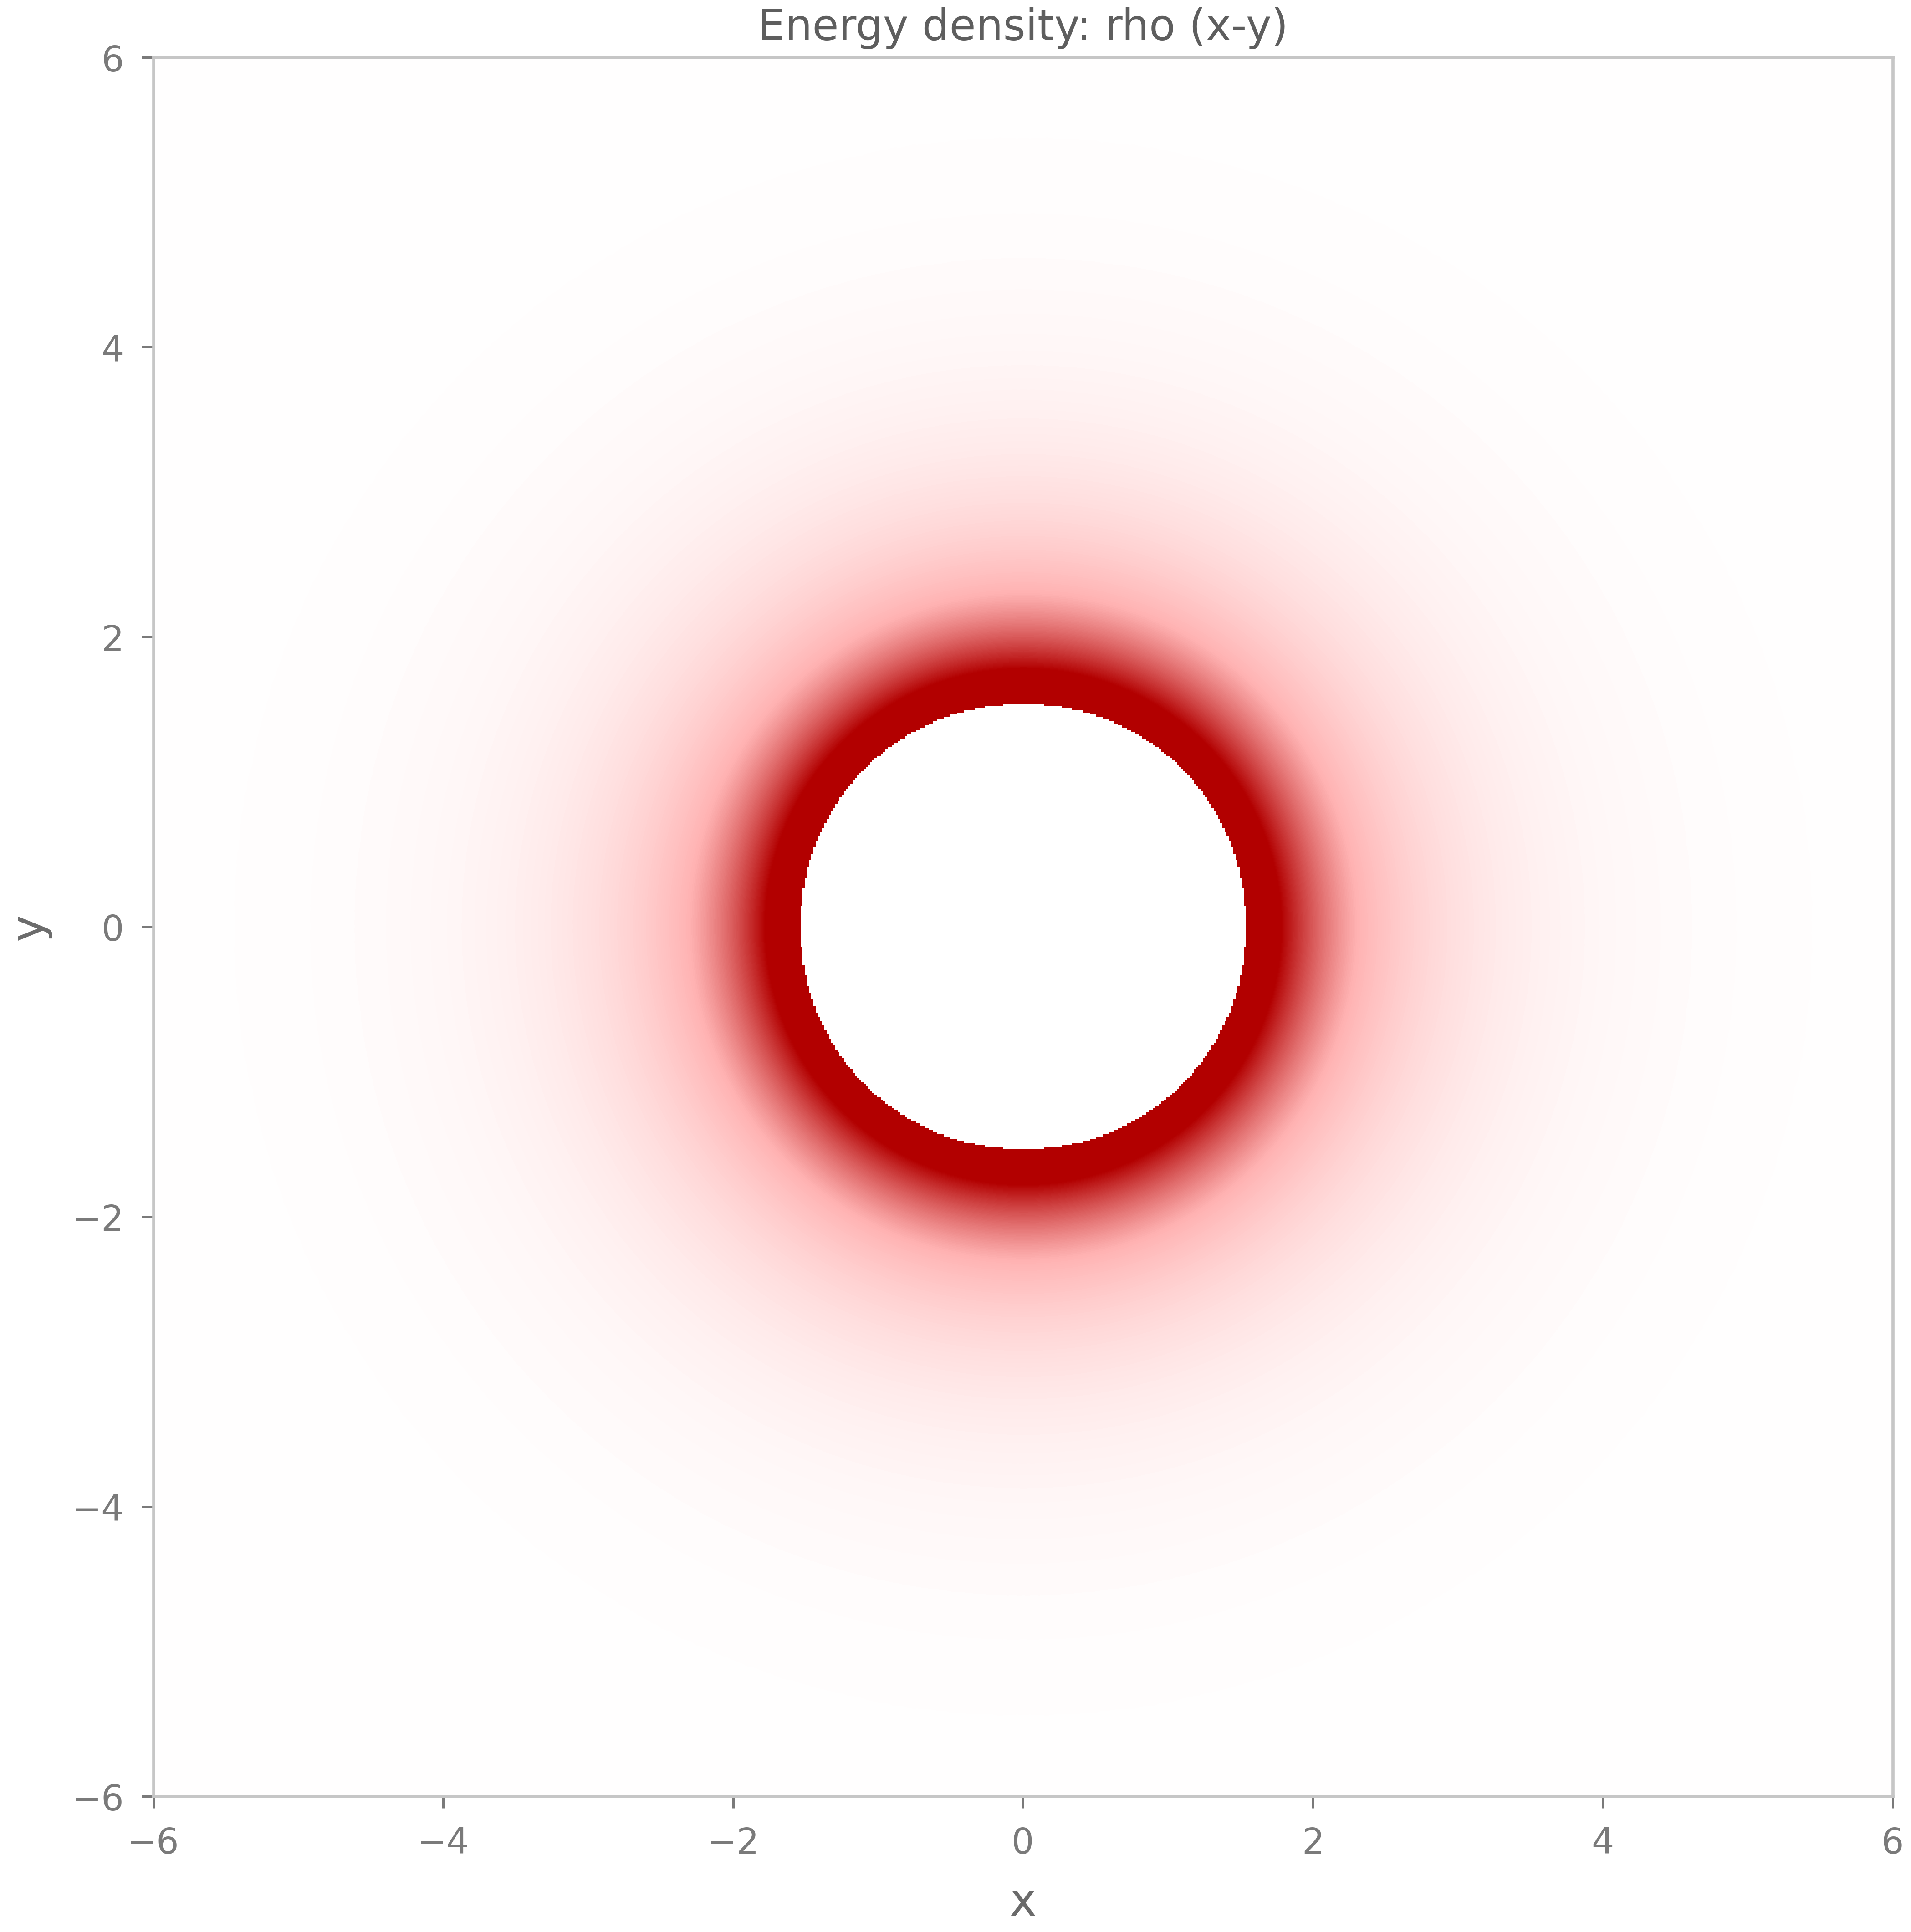
\includegraphics[width=\linewidth]{figures/domain_1_v_0p1_t_30p0_a0p970_b1p321_R00p000_XY_rho.png}
    \caption{Energy density \(\rho\) on the equatorial slice; the red annulus marks the positive-energy shell separating interior and exterior vacua.}
    \label{fig:d1-xy-rho}
  \end{subfigure}\hfill
  \begin{subfigure}[b]{0.46\textwidth}
    \centering
    \includegraphics[width=\linewidth]{figures/domain_1_v_0p1_t_30p0_a0p970_b1p321_R00p000_XY_WECmin.png}
    \caption{Minimum weak-energy--condition margin \(\mathrm{WEC}_{\min}\); the regenerated slice contains localized negative sectors rather than remaining everywhere non-negative, but the strongest residual obstruction still appears in the DEC diagnostic.}
    \label{fig:d1-xy-wecmin}
  \end{subfigure}

  \vspace{1ex}

  \begin{subfigure}[b]{0.46\textwidth}
    \centering
    \includegraphics[width=\linewidth]{figures/domain_1_v_0p1_t_30p0_a0p970_b1p321_R00p000_XY_NECmin.png}
    \caption{Minimum null-energy--condition margin \(\mathrm{NEC}_{\min}\), showing a localized deficit structure similar to the WEC diagnostic rather than a fully near-saturated shell.}
    \label{fig:d1-xy-necmin}
  \end{subfigure}

  \caption{Single-shell configuration, equatorial \(x\mbox{--}y\) slice at \(v=0.1\), \(t=30\).
  Colors are blue for negative values (violations), white near zero, and red for positive values.}
  \label{fig:d1-xy-energy-A}
\end{figure}

%-----------------------------------------------------
% Single shell: Energy conditions, XY slice (2 panels)
%-----------------------------------------------------
\begin{figure}[htbp]
  \centering
  \begin{subfigure}[b]{0.46\textwidth}
    \centering
    \includegraphics[width=\linewidth]{figures/domain_1_v_0p1_t_30p0_a0p970_b1p321_R00p000_XY_DECmargin.png}
    \caption{DEC margin, highlighting a narrow blue ring where tangential stresses exceed \(\rho\) in magnitude while the density itself remains positive.}
    \label{fig:d1-xy-decmargin}
  \end{subfigure}\hfill
  \begin{subfigure}[b]{0.46\textwidth}
    \centering
    \includegraphics[width=\linewidth]{figures/domain_1_v_0p1_t_30p0_a0p970_b1p321_R00p000_XY_SEC.png}
    \caption{Strong-energy--condition \(\SEC=\rho+p_1+p_2+p_3\) on the equatorial slice; the regenerated trace is sign-changing, although it remains less restrictive in aggregate than the DEC margin.}
    \label{fig:d1-xy-sec}
  \end{subfigure}
  \caption{Single-shell configuration, equatorial slice:
  diagnostics that identify the dominant residual constraint as the \DEC\ rather than the \WEC/\NEC.}
  \label{fig:d1-xy-energy-B}
\end{figure}

%-----------------------------------------------------
% Single shell: Energy conditions, XZ slice (3 panels)
%-----------------------------------------------------
\begin{figure}[htbp]
  \centering
  \begin{subfigure}[b]{0.46\textwidth}
    \centering
    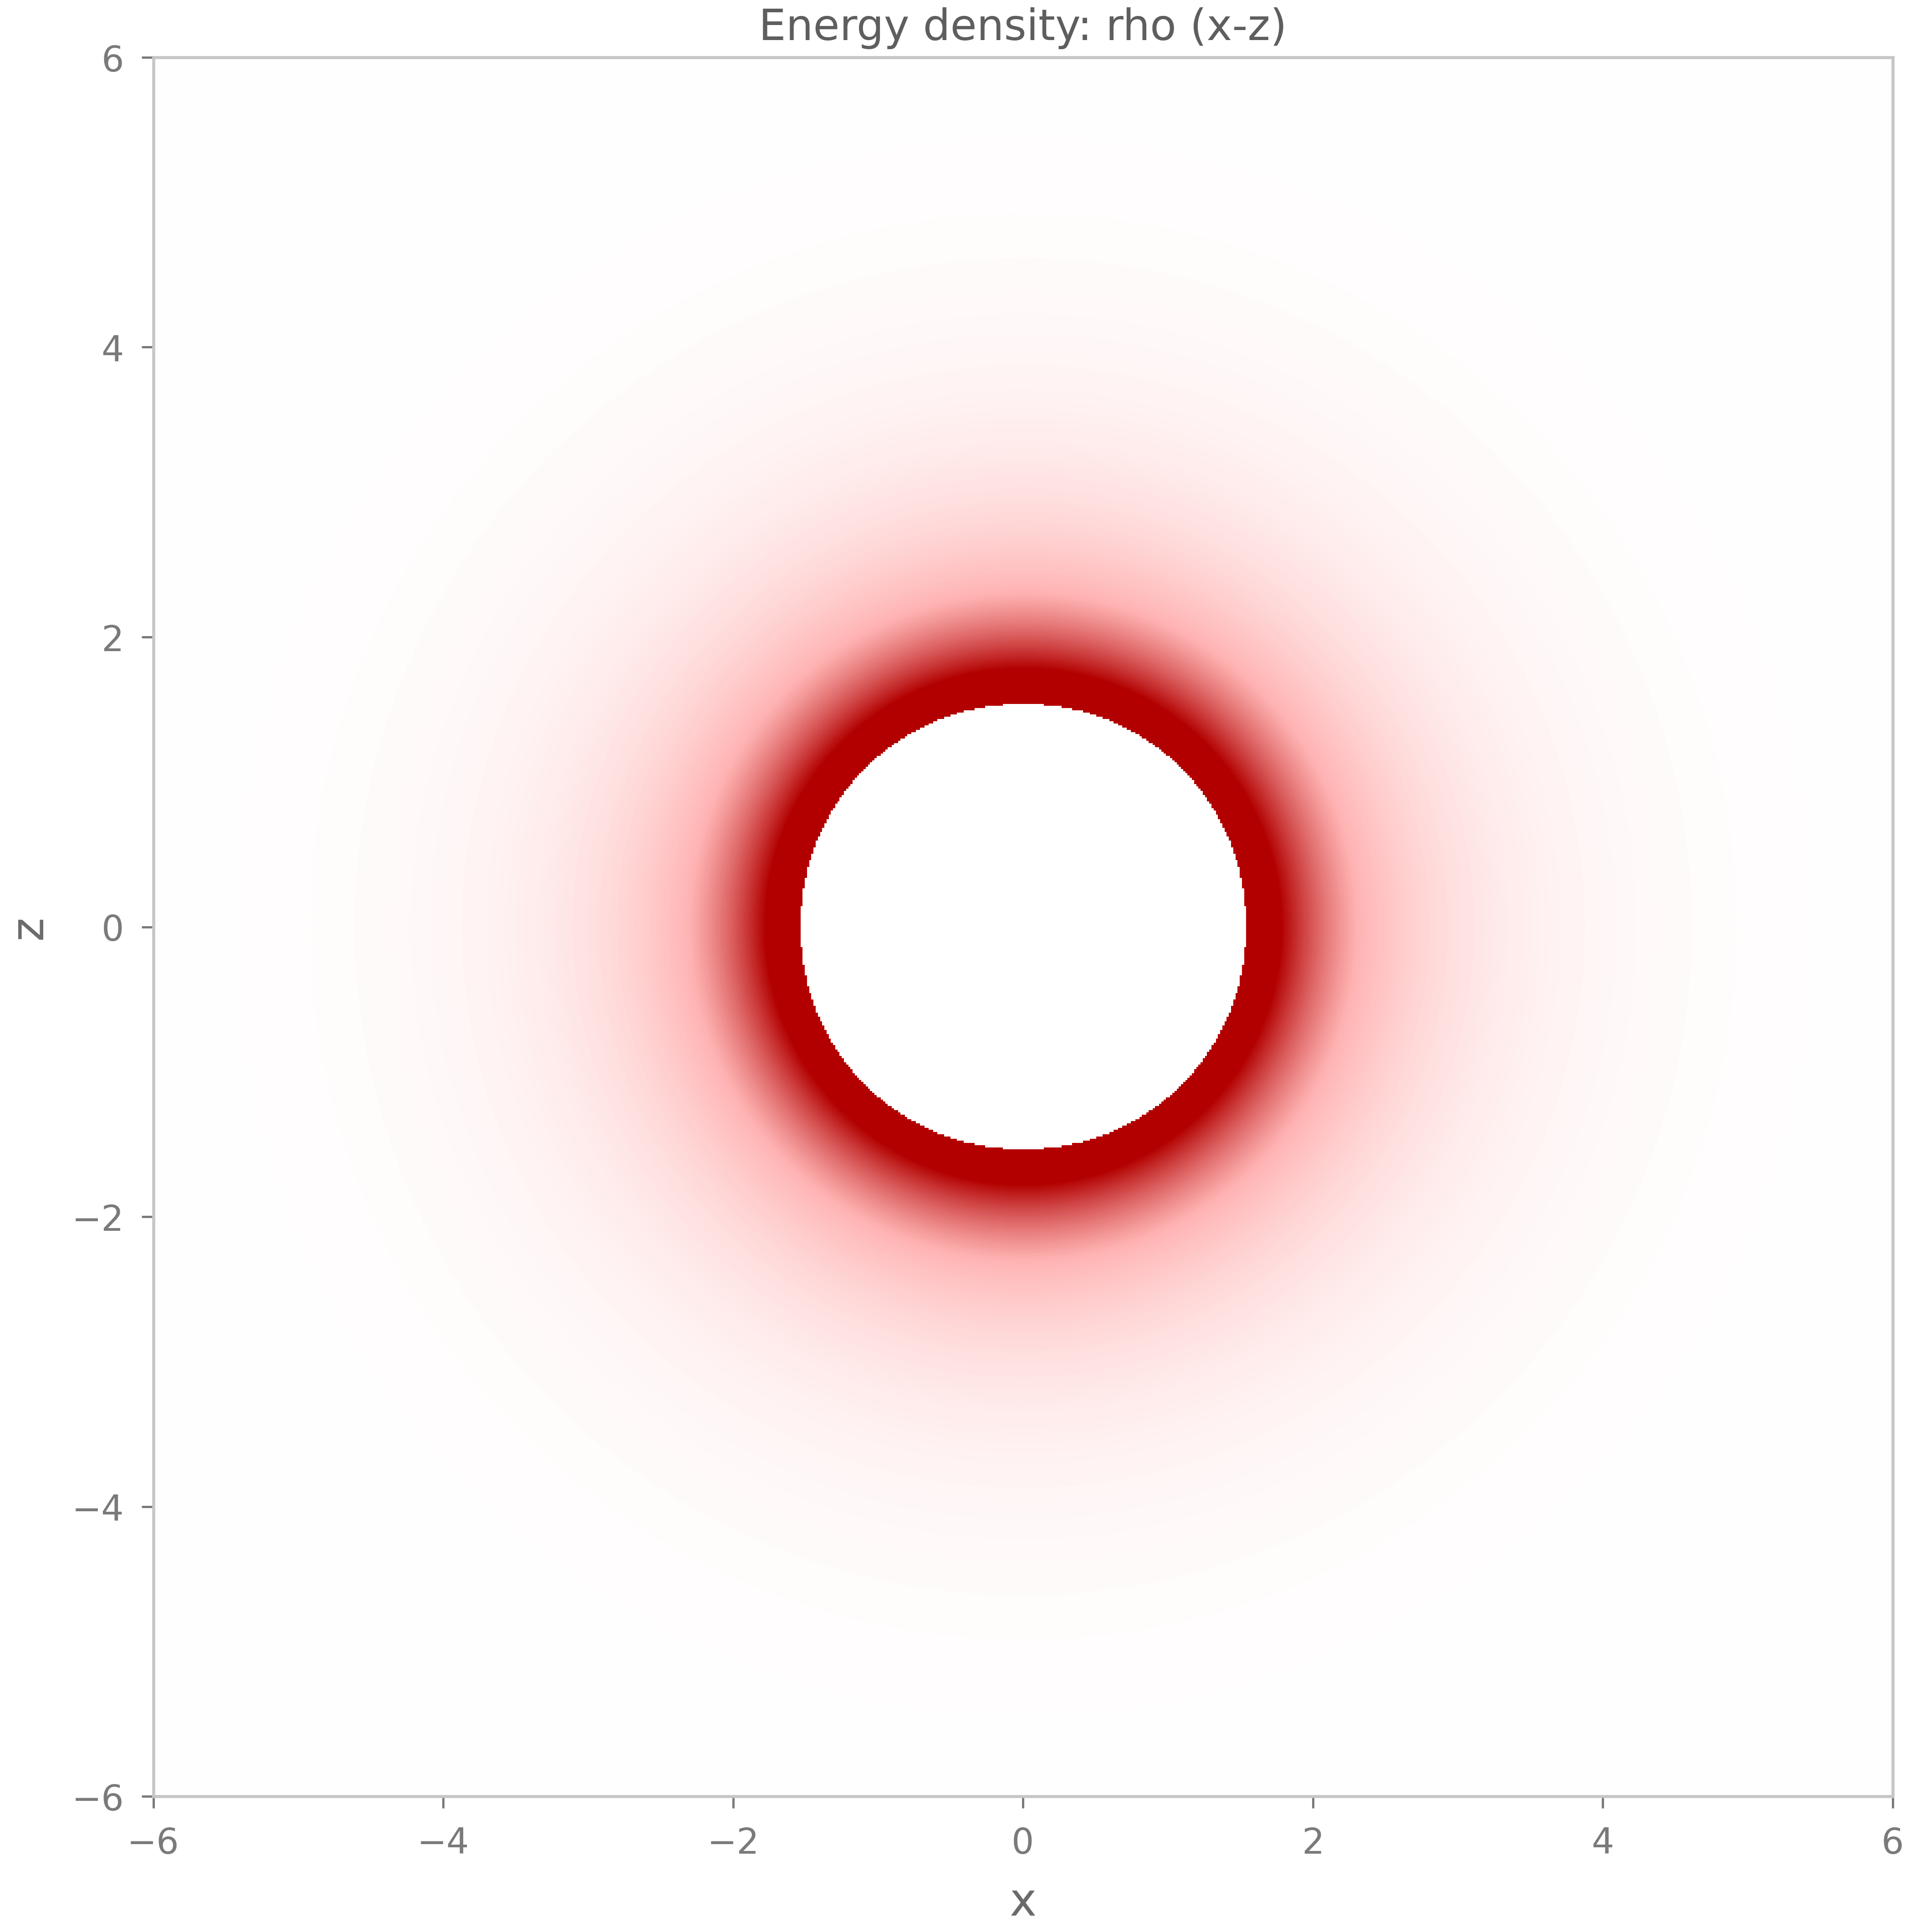
\includegraphics[width=\linewidth]{figures/domain_1_v_0p1_t_30p0_a0p970_b1p321_R00p000_XZ_rho.png}
    \caption{Energy density \(\rho\) on the meridional \(x\mbox{--}z\) slice; the thin red annulus shows the same single-shell structure in cross-section.}
    \label{fig:d1-xz-rho}
  \end{subfigure}\hfill
  \begin{subfigure}[b]{0.46\textwidth}
    \centering
    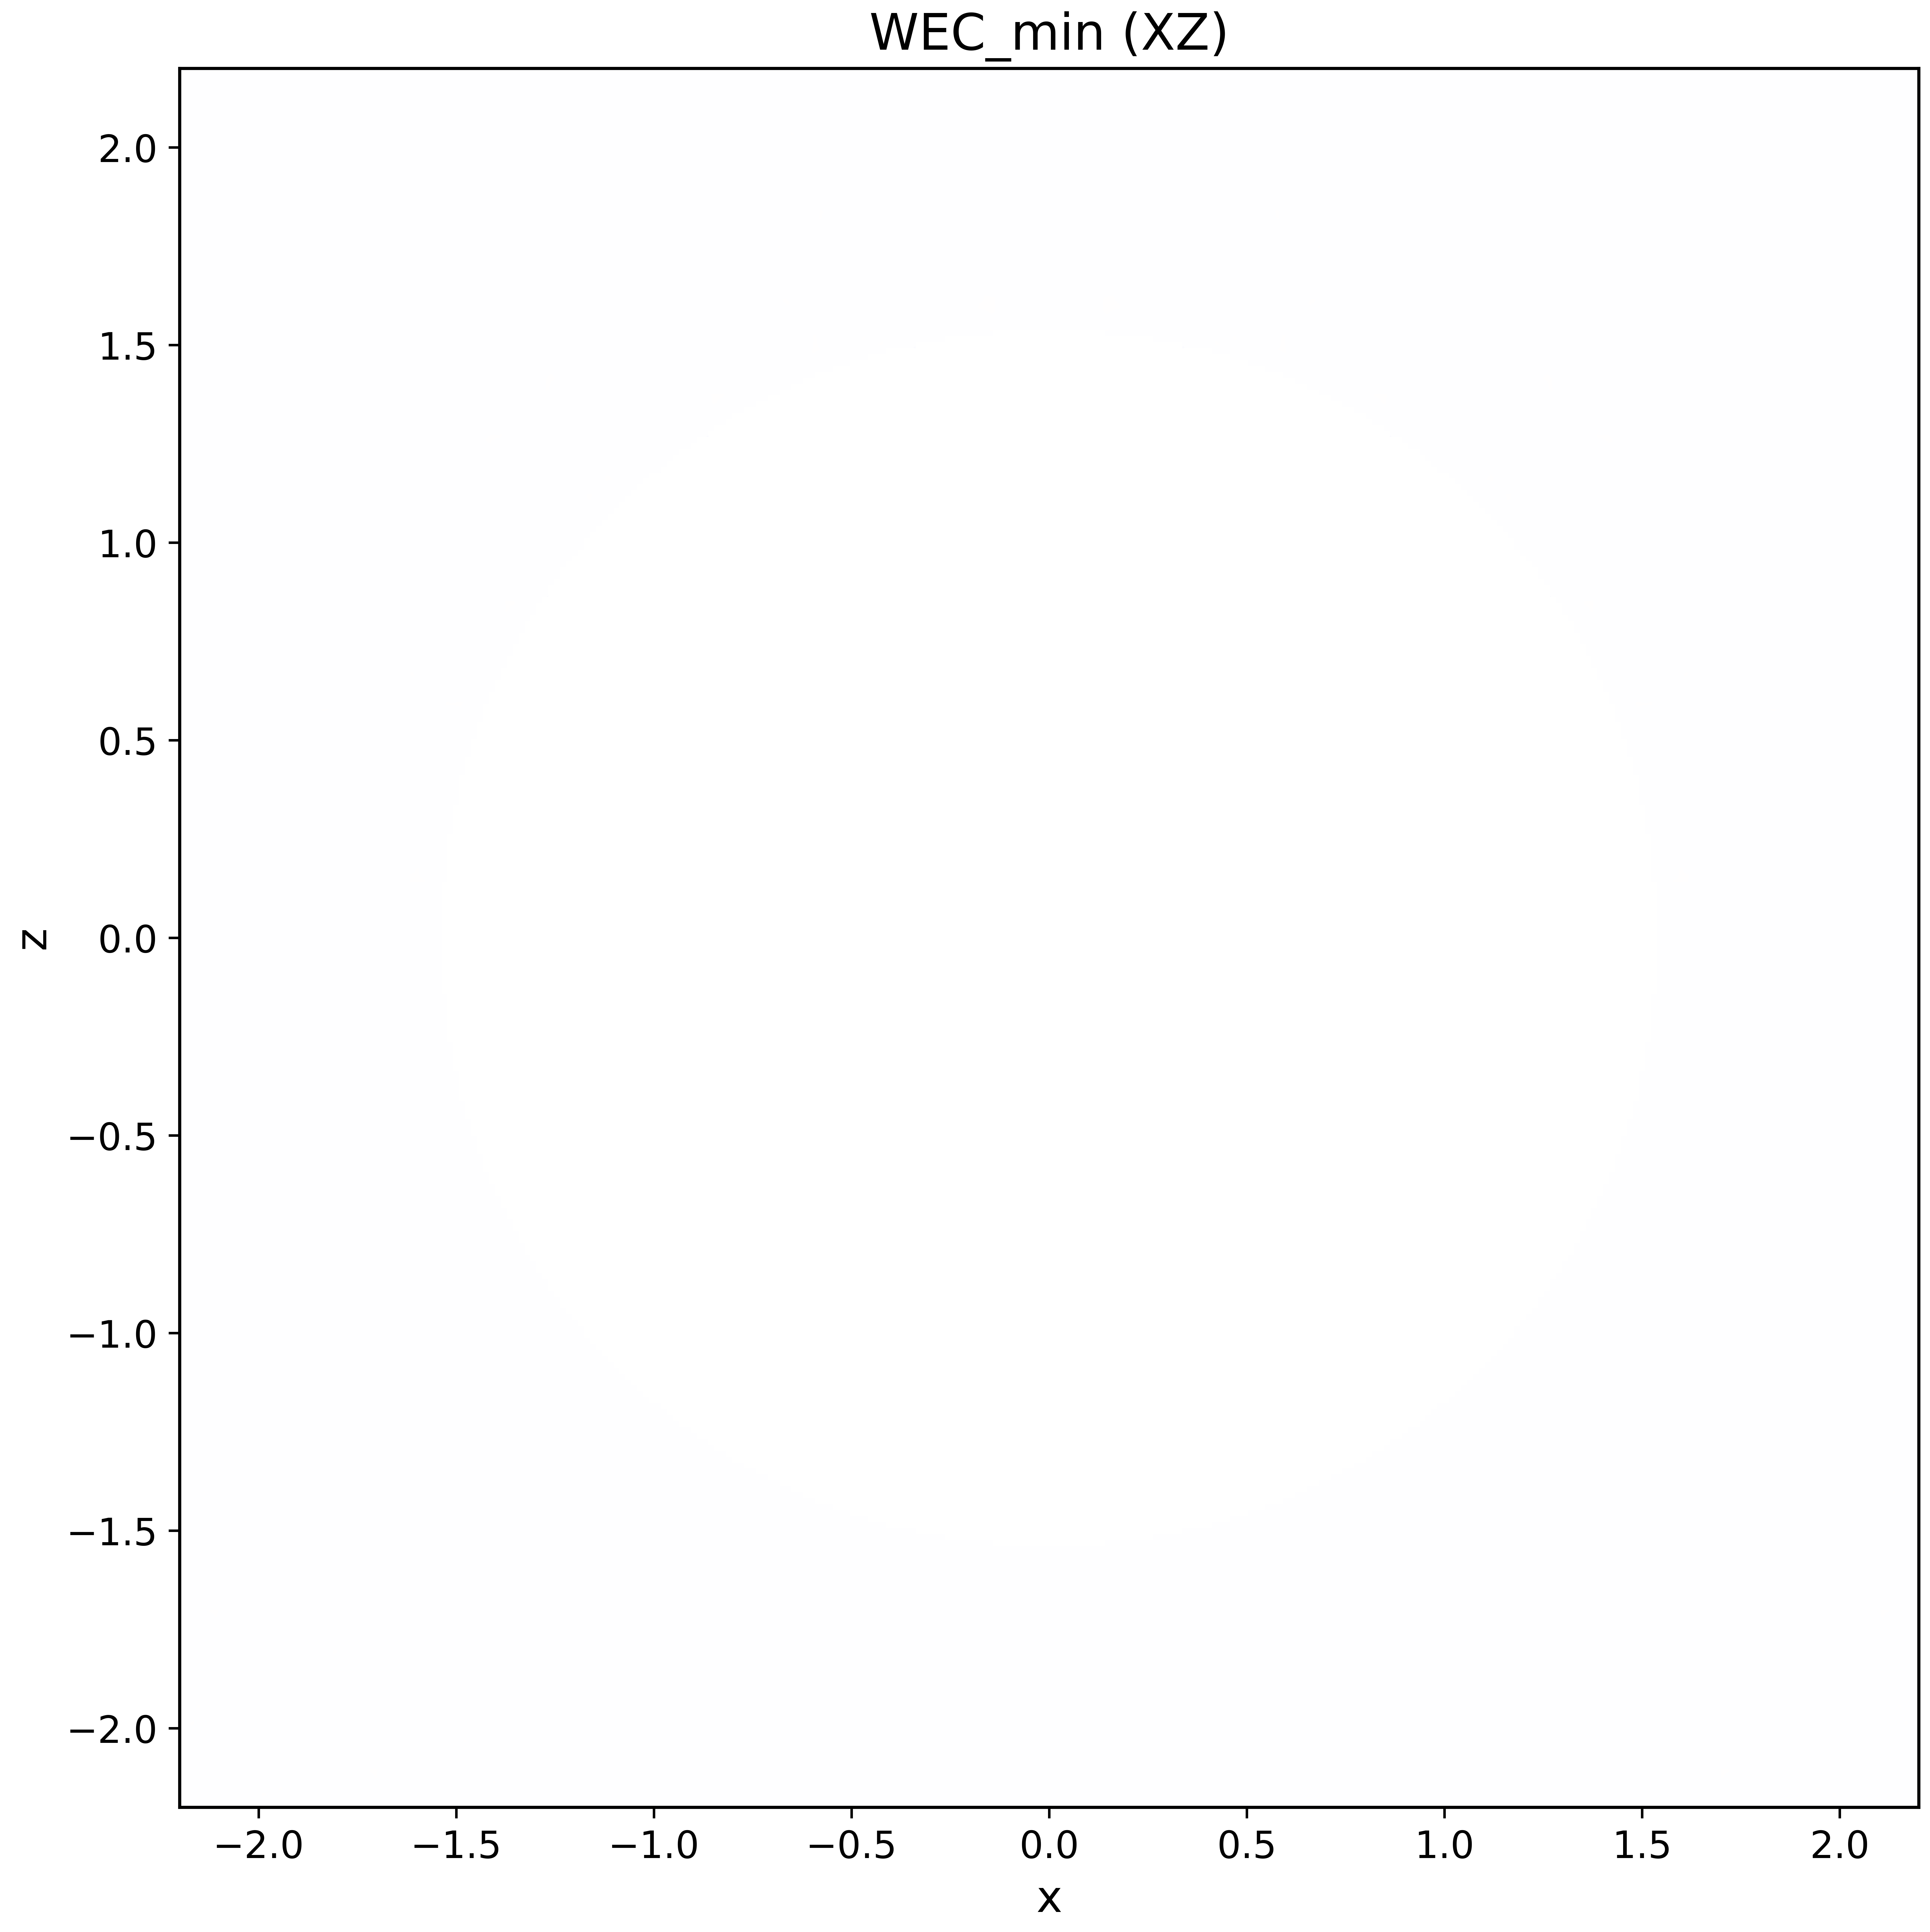
\includegraphics[width=\linewidth]{figures/domain_1_v_0p1_t_30p0_a0p970_b1p321_R00p000_XZ_WECmin.png}
    \caption{\(\mathrm{WEC}_{\min}\) on the meridional slice; the regenerated map shows localized negative sectors rather than a uniformly near-zero shell.}
    \label{fig:d1-xz-wecmin}
  \end{subfigure}

  \vspace{1ex}

  \begin{subfigure}[b]{0.46\textwidth}
    \centering
    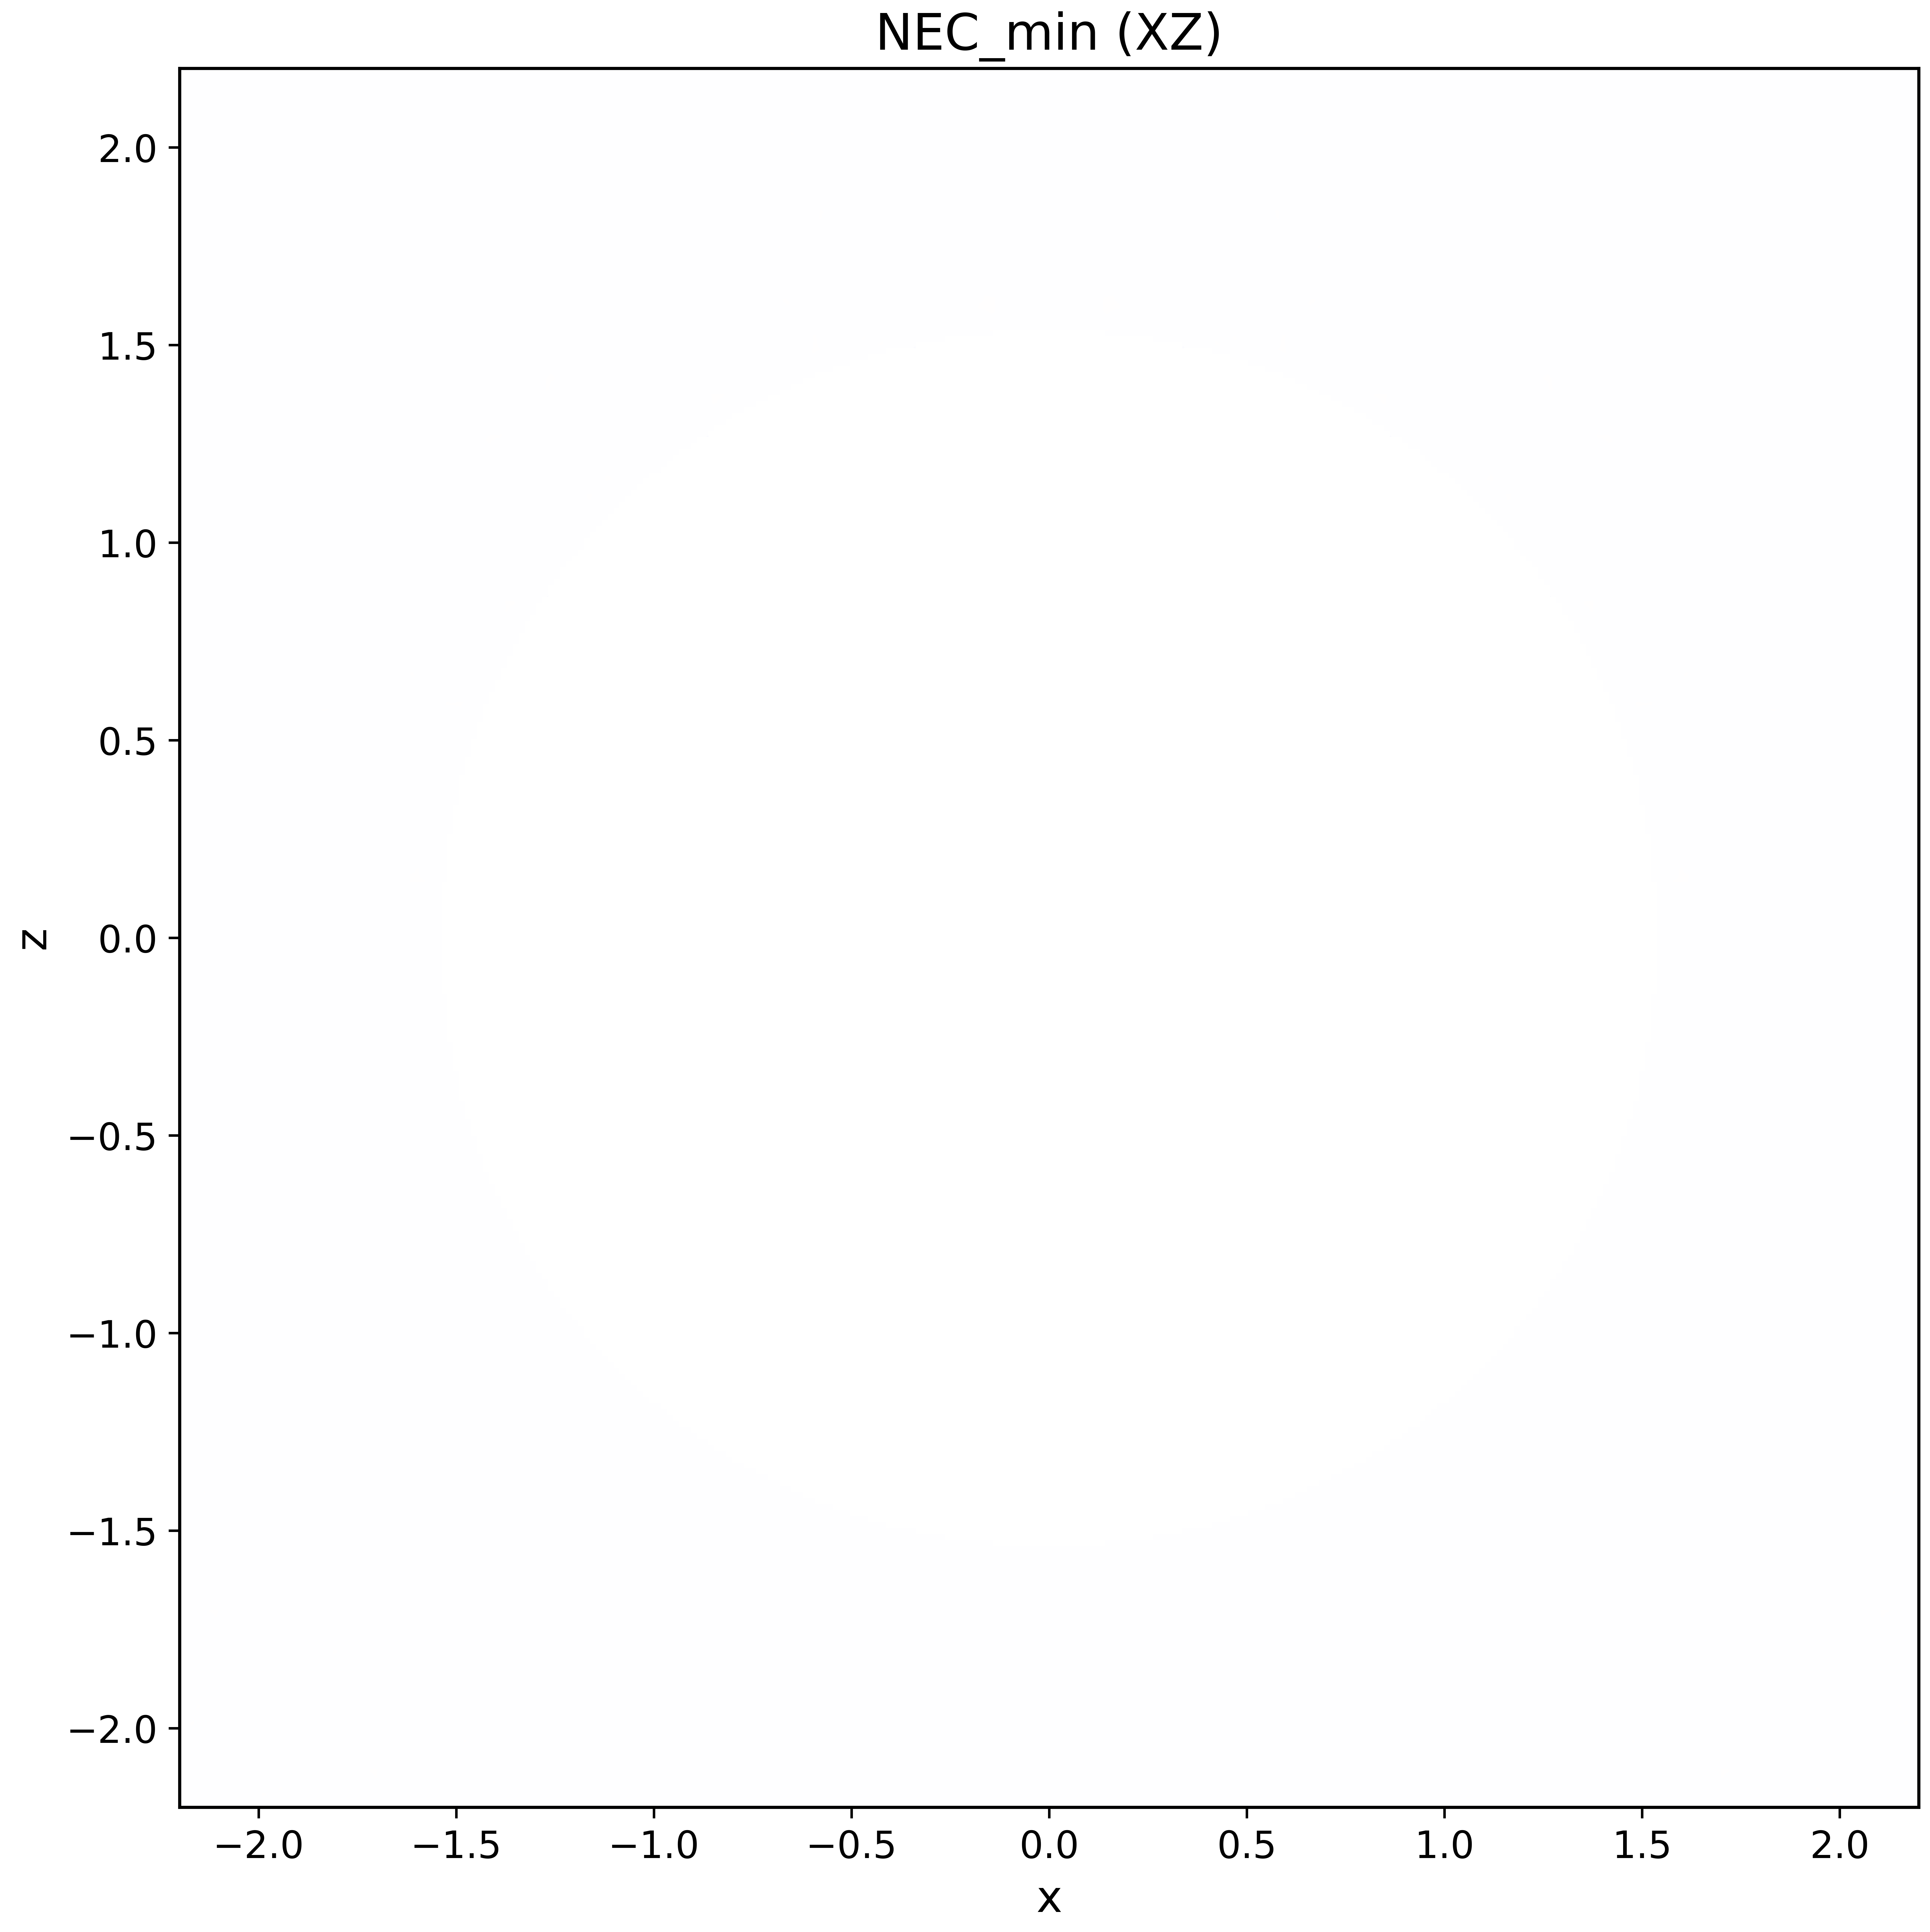
\includegraphics[width=\linewidth]{figures/domain_1_v_0p1_t_30p0_a0p970_b1p321_R00p000_XZ_NECmin.png}
    \caption{\(\mathrm{NEC}_{\min}\), showing the same localized deficit structure as the WEC diagnostic on the meridional slice.}
    \label{fig:d1-xz-necmin}
  \end{subfigure}

  \caption{Single-shell configuration, meridional \(x\mbox{--}z\) slice:
  density and minimum \WEC/\NEC\ margins, complementary to the equatorial view in Fig.~\ref{fig:d1-xy-energy-A}.}
  \label{fig:d1-xz-energy-A}
\end{figure}

%-----------------------------------------------------
% Single shell: Energy conditions, XZ slice (2 panels)
%-----------------------------------------------------
\begin{figure}[htbp]
  \centering
  \begin{subfigure}[b]{0.46\textwidth}
    \centering
    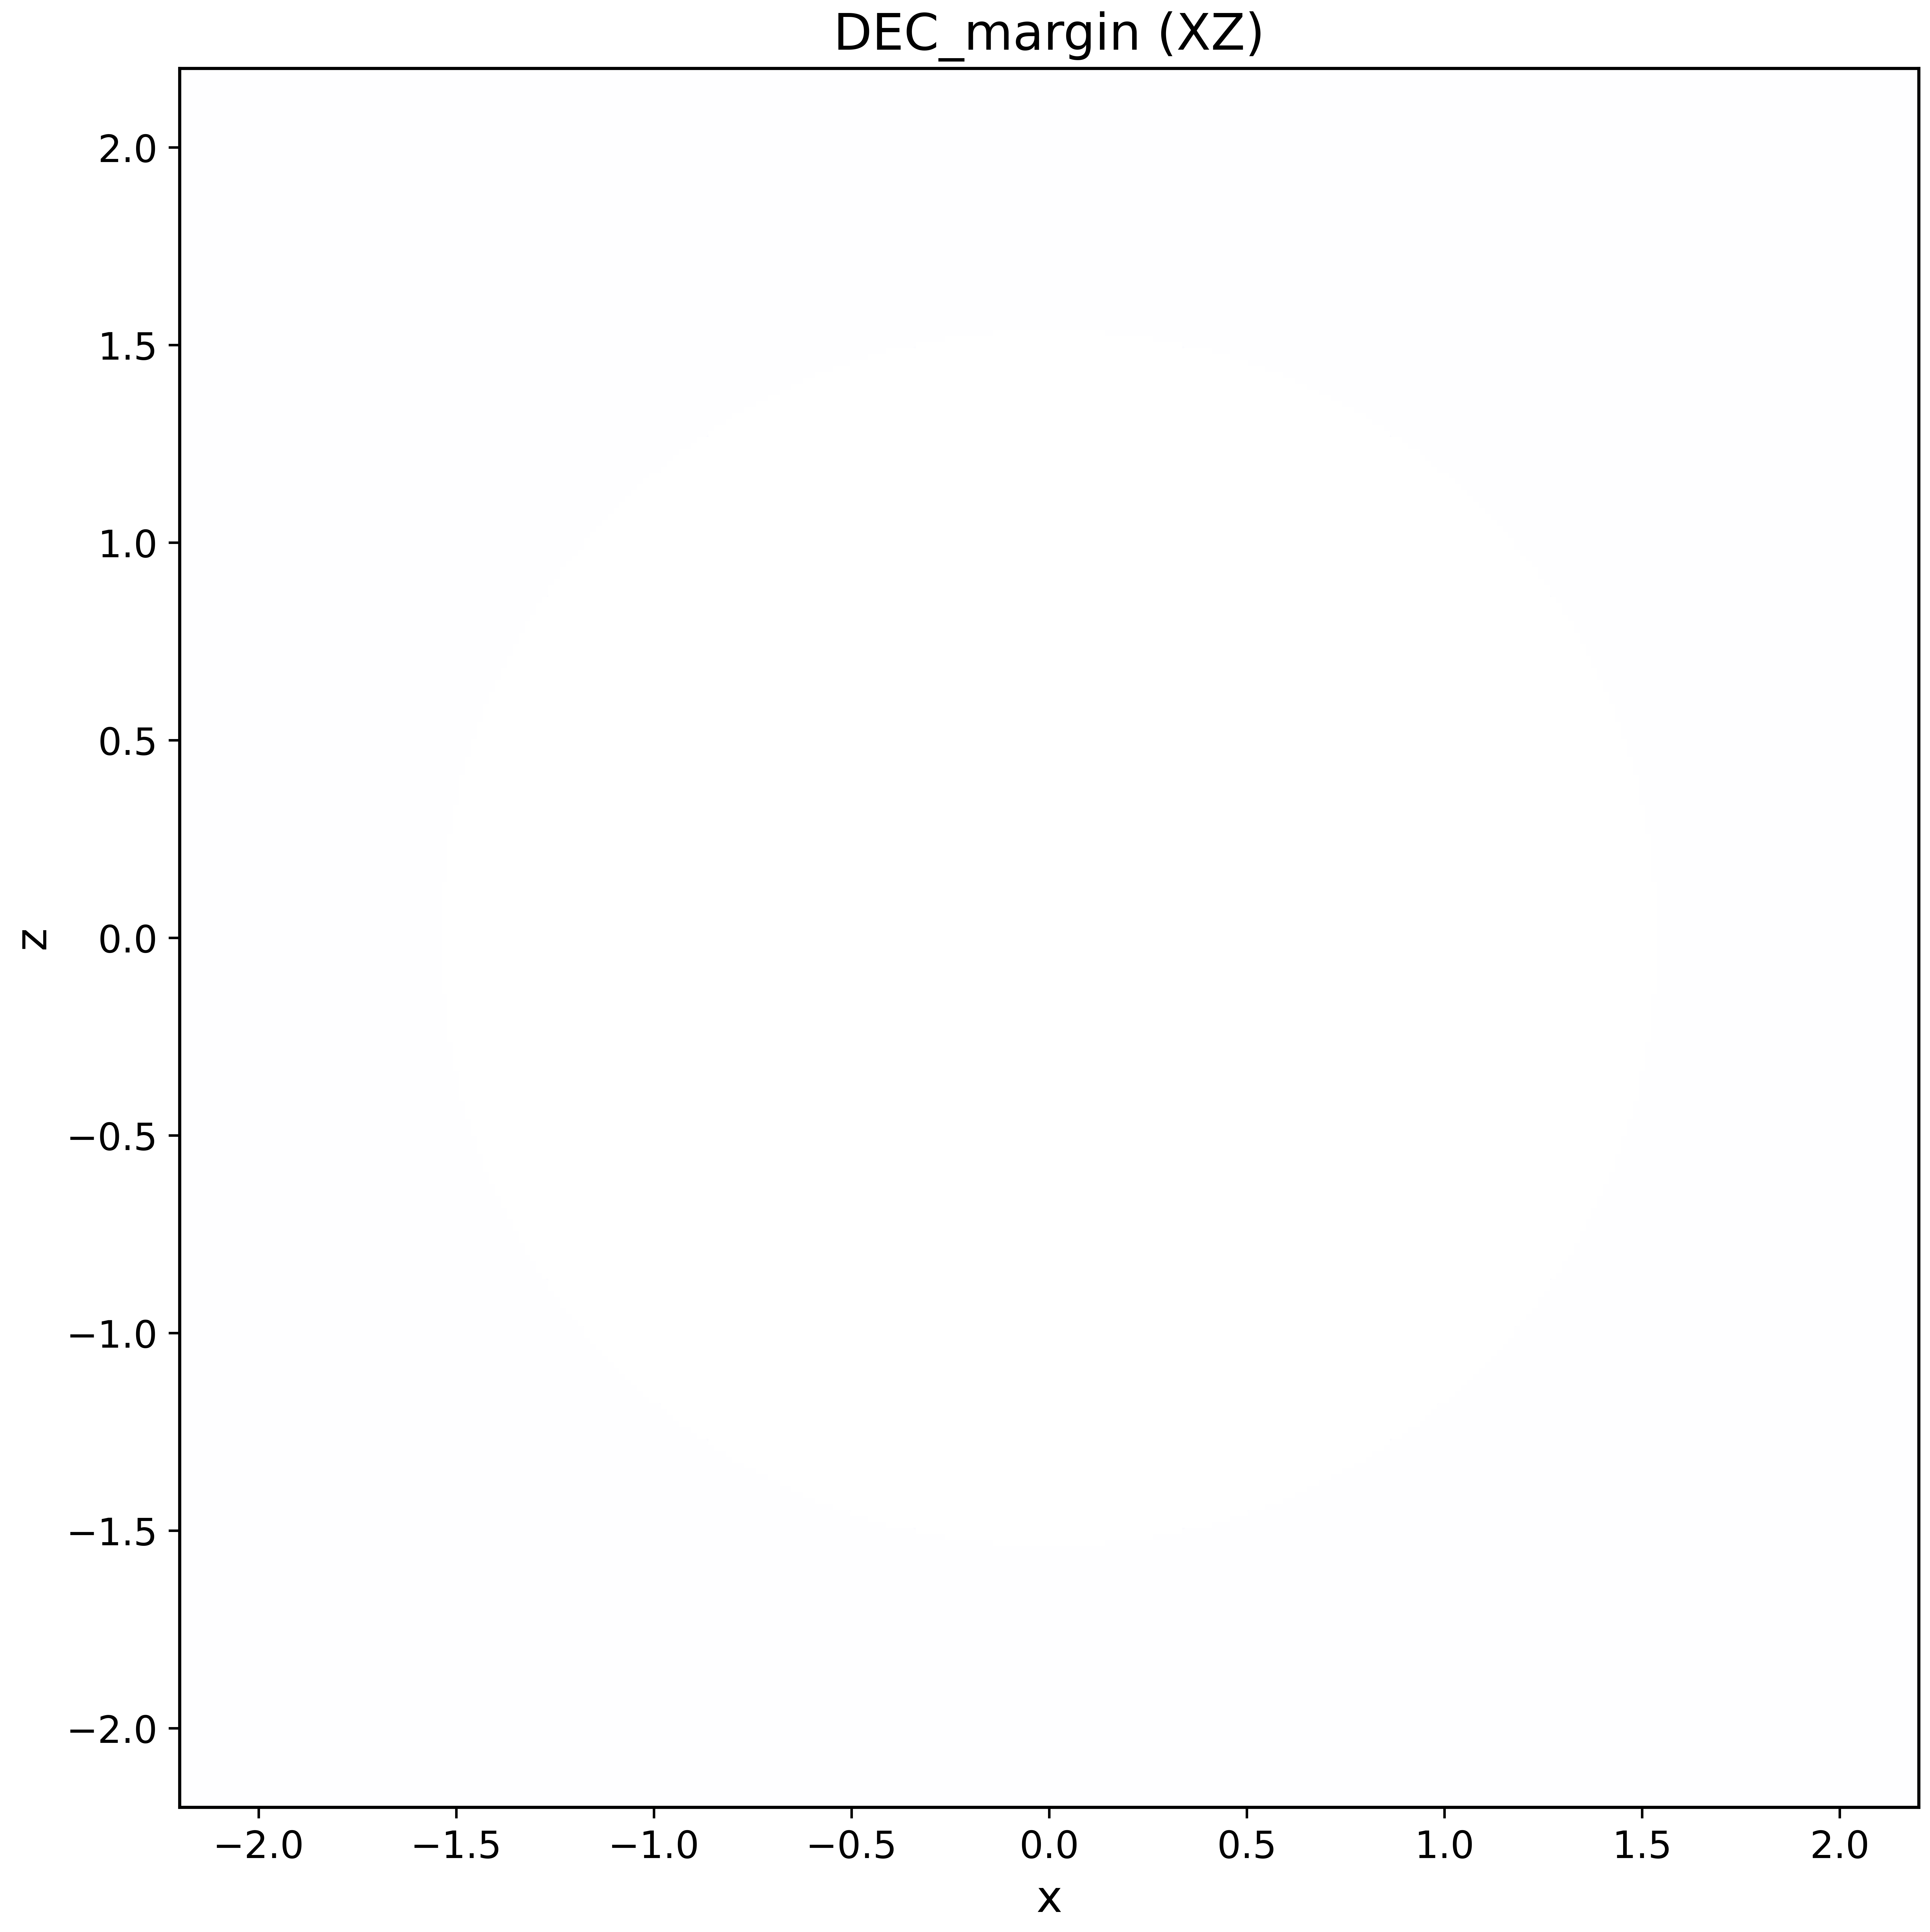
\includegraphics[width=\linewidth]{figures/domain_1_v_0p1_t_30p0_a0p970_b1p321_R00p000_XZ_DECmargin.png}
    \caption{DEC margin, again exhibiting a thin ring of violation closely aligned with the shell interfaces.}
    \label{fig:d1-xz-decmargin}
  \end{subfigure}\hfill
  \begin{subfigure}[b]{0.46\textwidth}
    \centering
    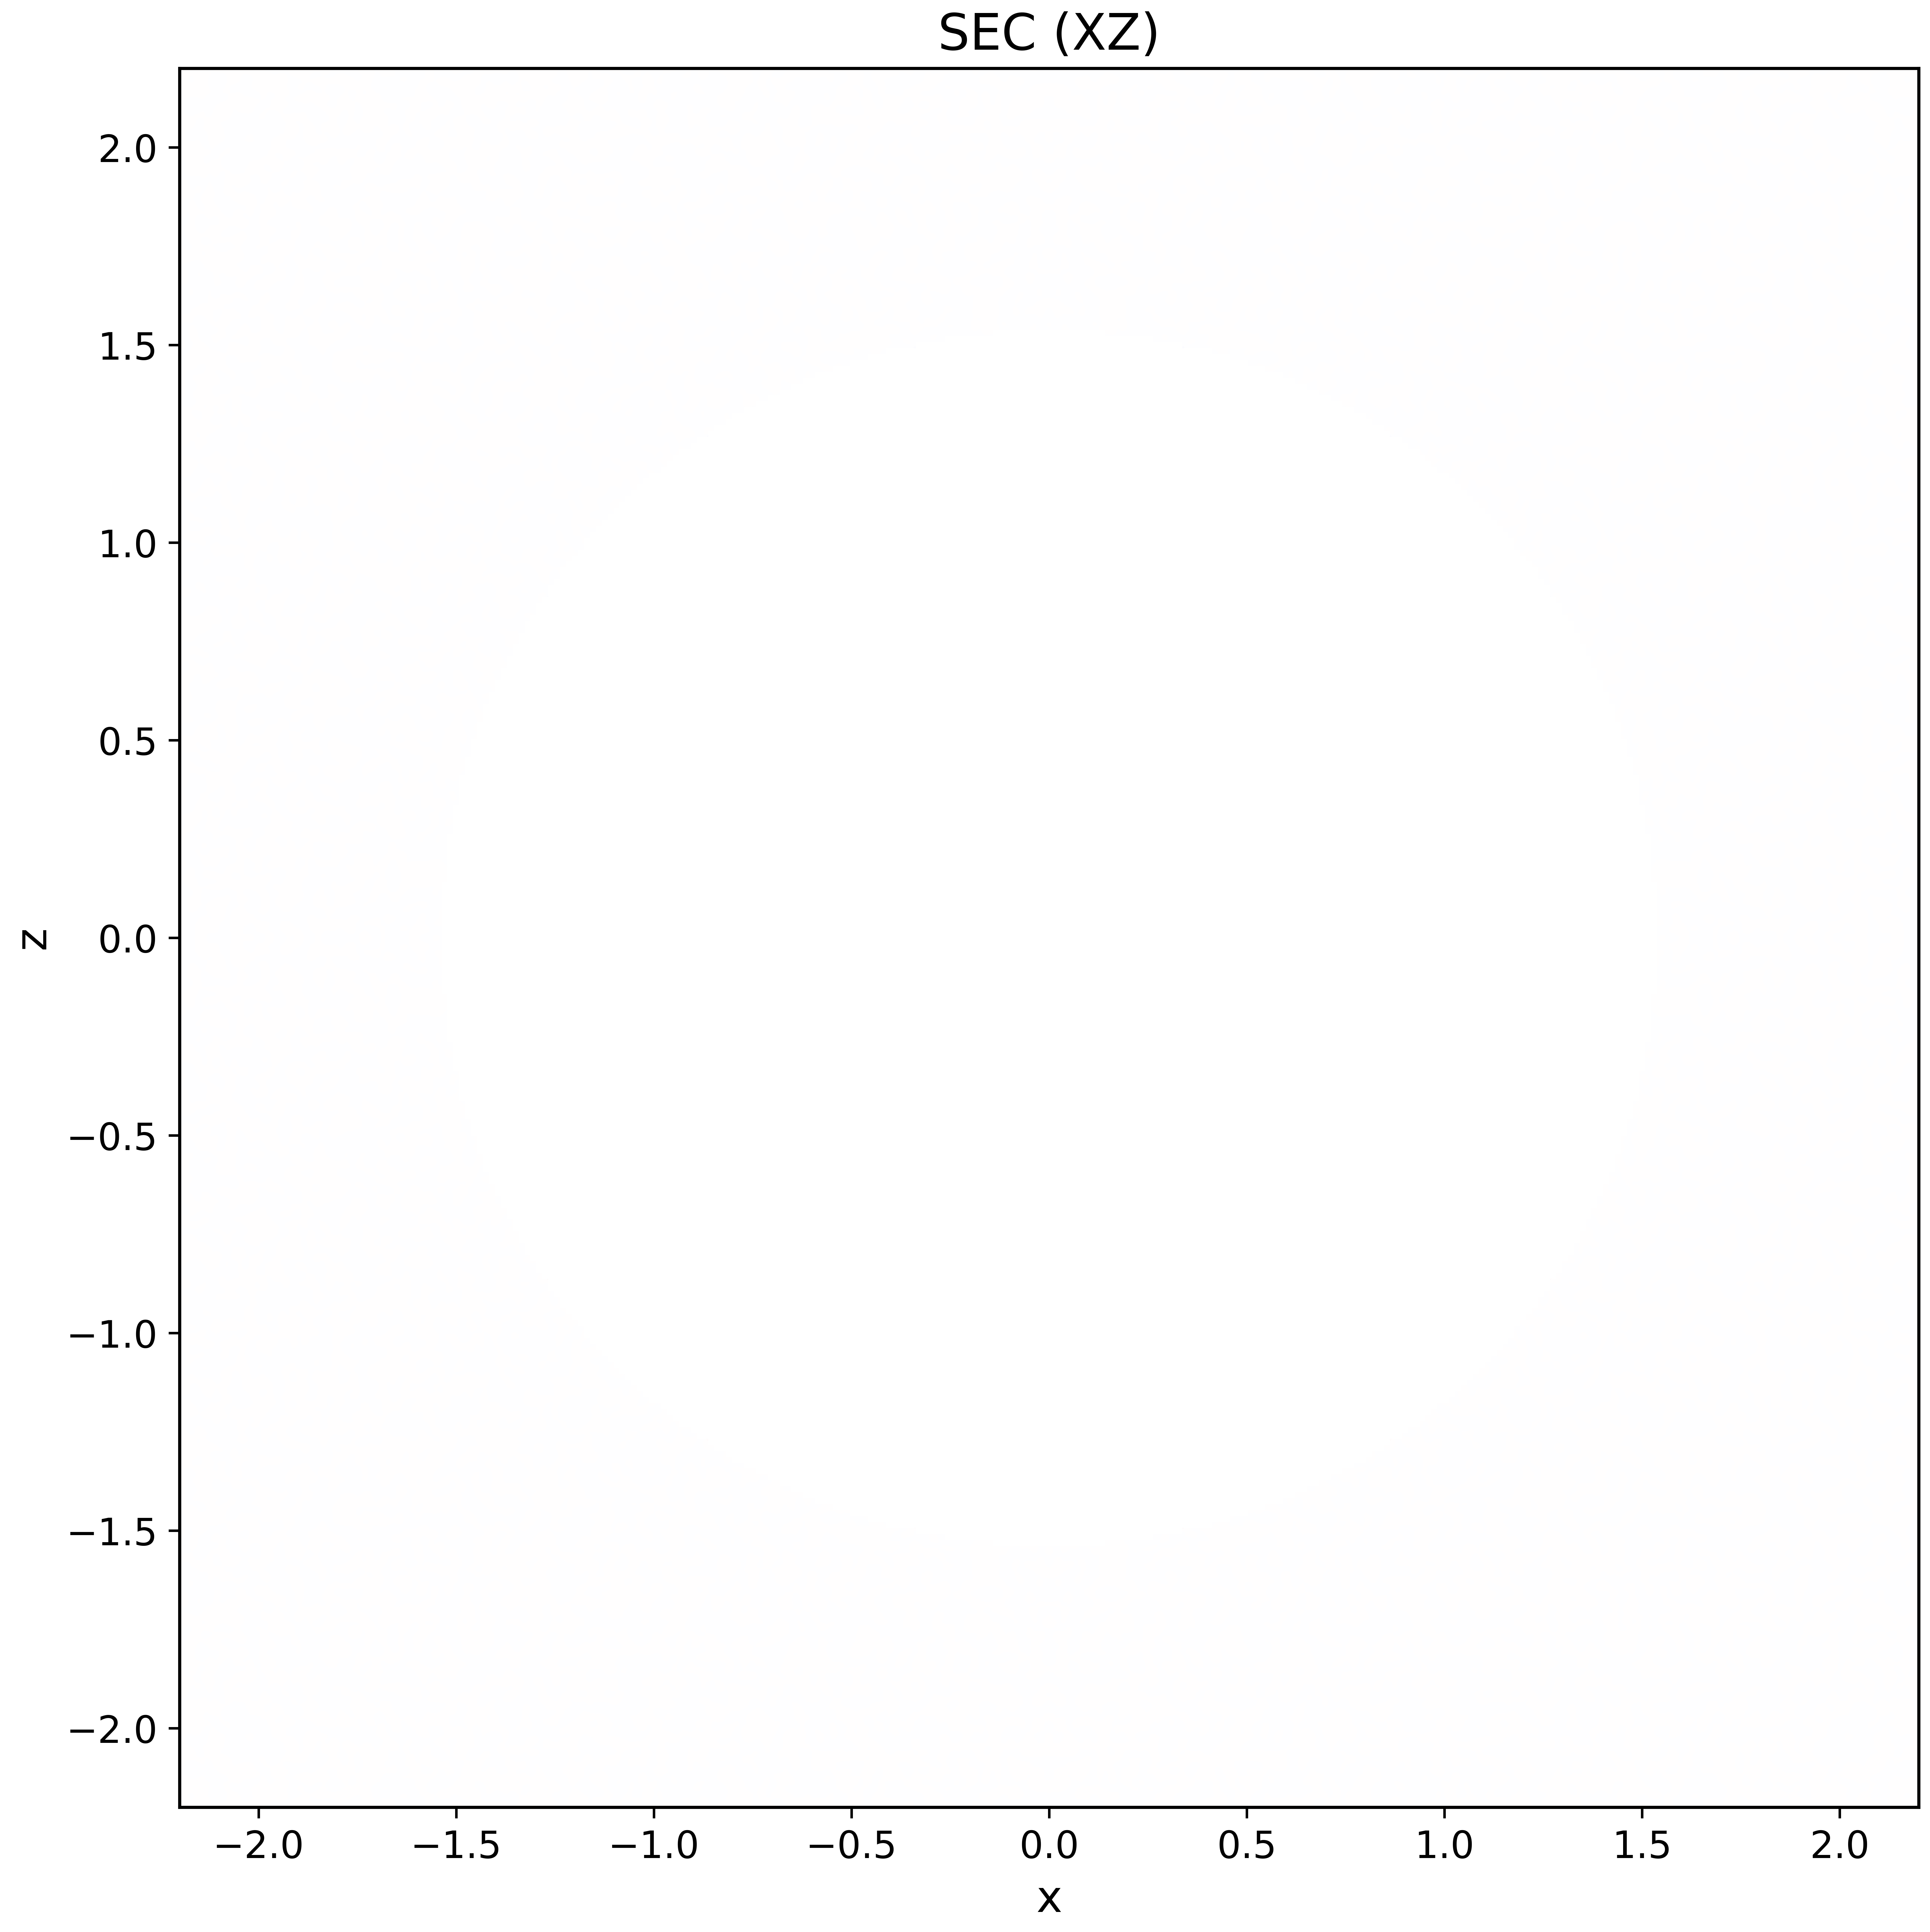
\includegraphics[width=\linewidth]{figures/domain_1_v_0p1_t_30p0_a0p970_b1p321_R00p000_XZ_SEC.png}
    \caption{\(\SEC\) on the meridional slice; the regenerated trace is mixed rather than uniformly positive, but its aggregate success fraction still exceeds the DEC success fraction.}
    \label{fig:d1-xz-sec}
  \end{subfigure}

  \caption{Single-shell configuration, meridional slice:
  \DEC\ and \SEC\ diagnostics revealing that residual stress anisotropies are tightly localized.}
  \label{fig:d1-xz-energy-B}
\end{figure}

%-----------------------------------------------------
% Double shell: Energy conditions, XY slice (3 panels)
%-----------------------------------------------------
\begin{figure}[htbp]
  \centering
  \begin{subfigure}[b]{0.46\textwidth}
    \centering
    
\includegraphics[width=\linewidth]{figures/domain_2_v_0p1_t_30p0_a1p848_b1p135_R01p292_XY_rho.png}
    \caption{Energy density \(\rho\) on the equatorial slice for the double-shell seed; the positive-energy region now spans a broader annulus.}
    \label{fig:d2-xy-rho}
  \end{subfigure}\hfill
  \begin{subfigure}[b]{0.46\textwidth}
    \centering
    
\includegraphics[width=\linewidth]{figures/domain_2_v_0p1_t_30p0_a1p848_b1p135_R01p292_XY_WECmin.png}
    \caption{\(\mathrm{WEC}_{\min}\), showing a central blue region and inner-interface band where the WEC is violated while the outer shell remains close to saturation.}
    \label{fig:d2-xy-wecmin}
  \end{subfigure}

  \vspace{1ex}

  \begin{subfigure}[b]{0.46\textwidth}
    \centering
    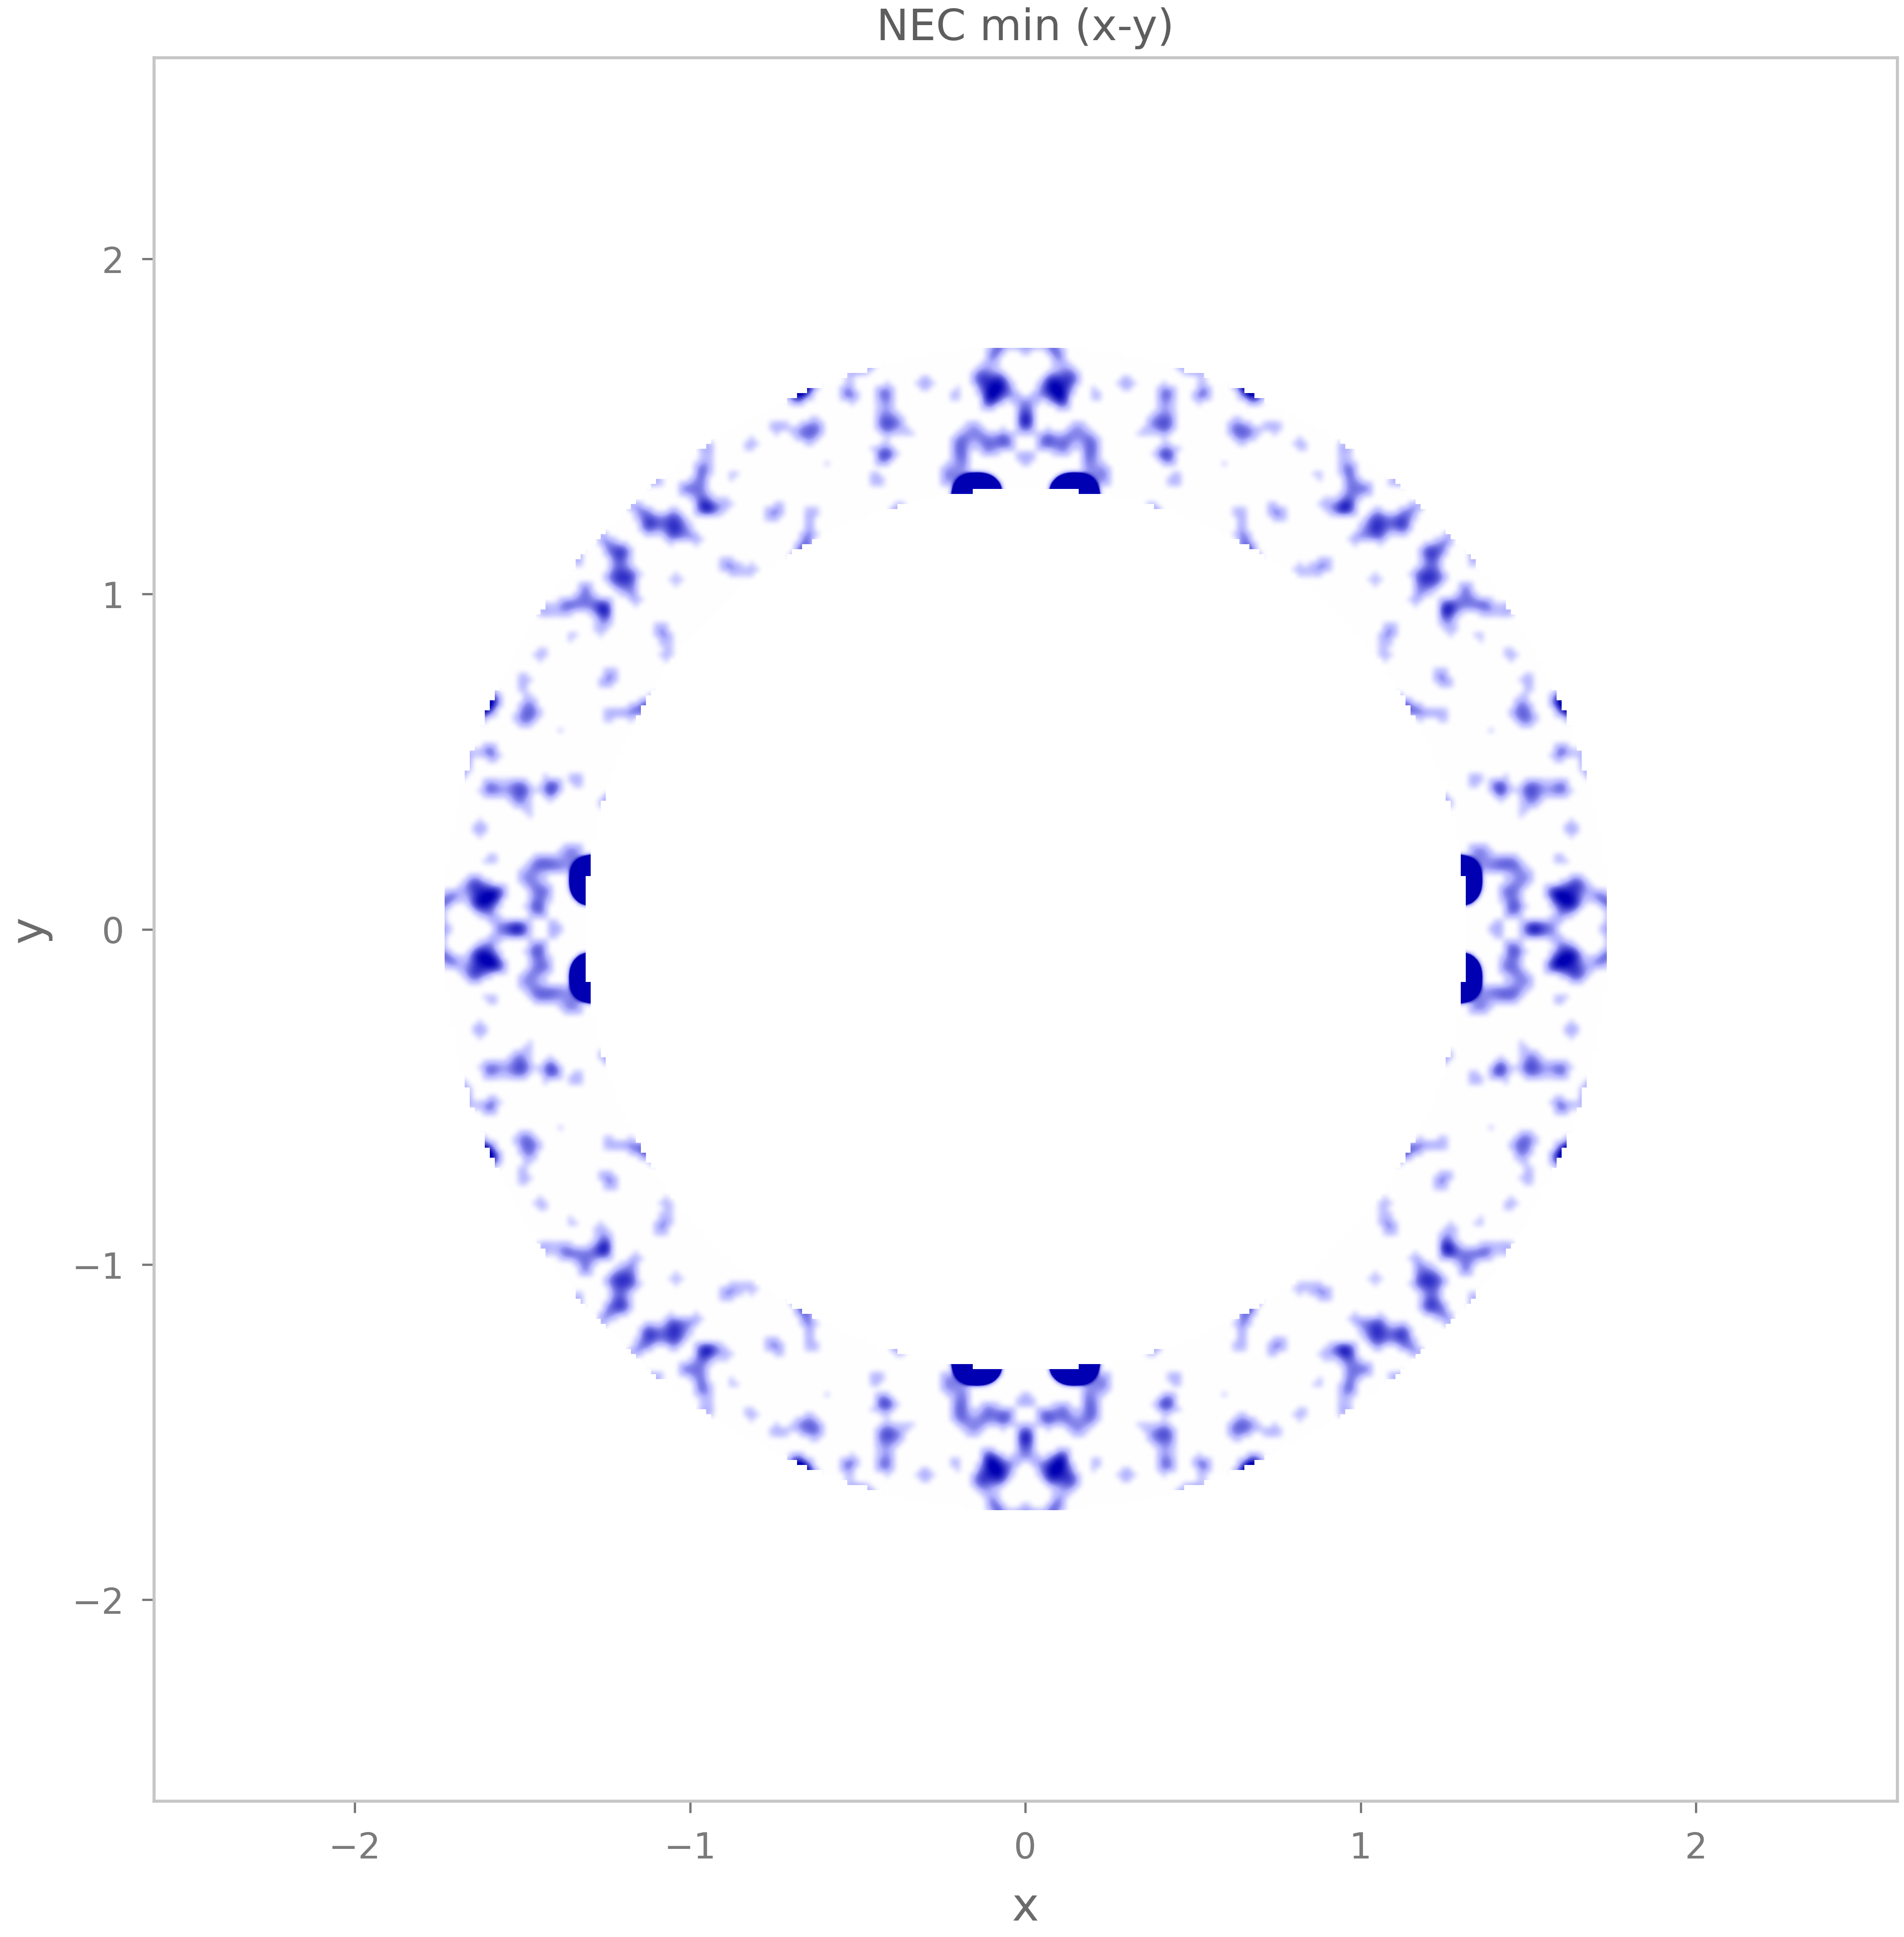
\includegraphics[width=\linewidth]{figures/domain_2_v_0p1_t_30p0_a1p848_b1p135_R01p292_XY_NECmin.png}
    \caption{\(\mathrm{NEC}_{\min}\), with a similar central deficit pattern, indicating that the inner vacuum interface is the main source of WEC/NEC violations.}
    \label{fig:d2-xy-necmin}
  \end{subfigure}

  \caption{Double-shell configuration, equatorial \(x\mbox{--}y\) slice:
  density and minimum \WEC/\NEC\ margins, illustrating how the extra interface changes where violations concentrate.}
  \label{fig:d2-xy-energy-A}
\end{figure}

%-----------------------------------------------------
% Double shell: Energy conditions, XY slice (2 panels)
%-----------------------------------------------------
\begin{figure}[htbp]
  \centering
  \begin{subfigure}[b]{0.46\textwidth}
    \centering
    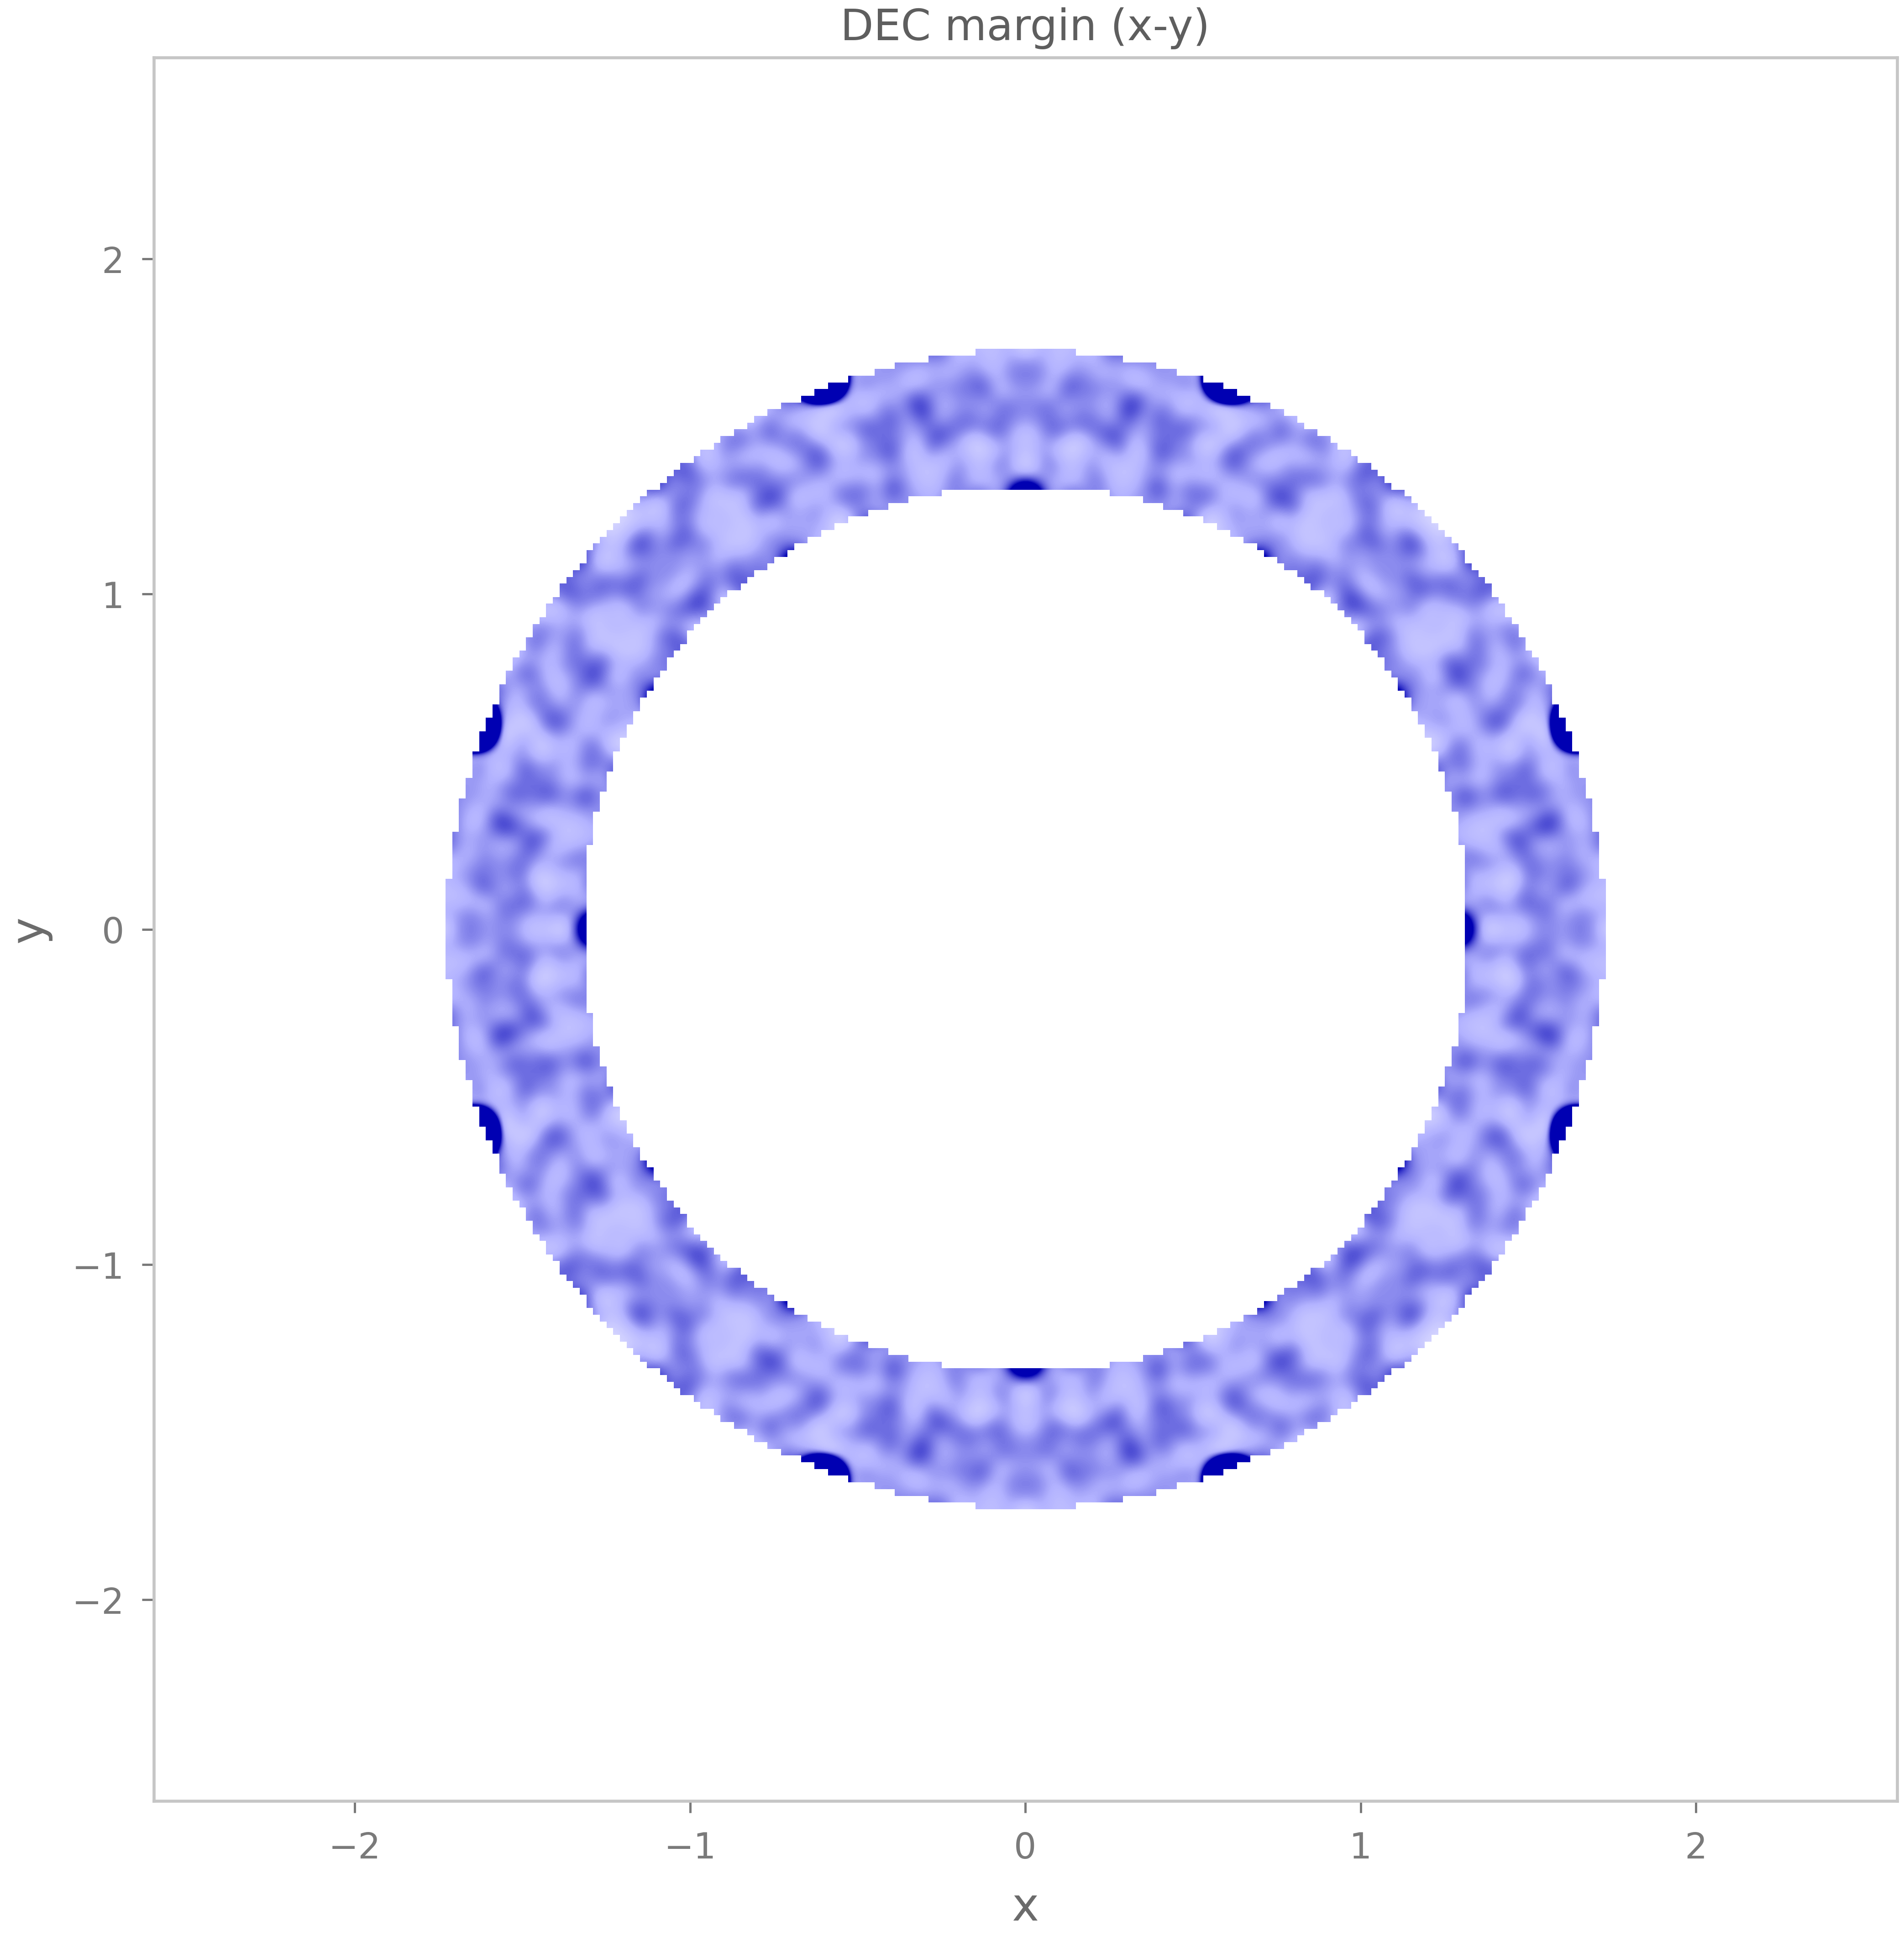
\includegraphics[width=\linewidth]{figures/domain_2_v_0p1_t_30p0_a1p848_b1p135_R01p292_XY_DECmargin.png}
    \caption{DEC margin, emphasising that the strongest violations are again tangential-stress dominated and most pronounced near the inner shell.}
    \label{fig:d2-xy-decmargin}
  \end{subfigure}\hfill
  \begin{subfigure}[b]{0.46\textwidth}
    \centering
    
\includegraphics[width=\linewidth]{figures/domain_2_v_0p1_t_30p0_a1p848_b1p135_R01p292_XY_SEC.png}
    \caption{\(\SEC\) on the equatorial slice; the trace is mixed rather than uniformly positive, but its deficits remain milder in aggregate than the corresponding DEC deficits.}
    \label{fig:d2-xy-sec}
  \end{subfigure}

  \caption{Double-shell configuration, equatorial slice:
  \DEC\ and \SEC\ diagnostics highlighting the trade-off between curvature redistribution and localized central deficits.}
  \label{fig:d2-xy-energy-B}
\end{figure}

%-----------------------------------------------------
% Double shell: Energy conditions, XZ slice (3 panels)
%-----------------------------------------------------
\begin{figure}[htbp]
  \centering
  \begin{subfigure}[b]{0.46\textwidth}
    \centering
    
\includegraphics[width=\linewidth]{figures/domain_2_v_0p1_t_30p0_a1p848_b1p135_R01p292_XZ_rho.png}
    \caption{Energy density \(\rho\) on the meridional slice; the outer shell is clearly visible, while the inner cavity remains vacuum.}
    \label{fig:d2-xz-rho}
  \end{subfigure}\hfill
  \begin{subfigure}[b]{0.46\textwidth}
    \centering
    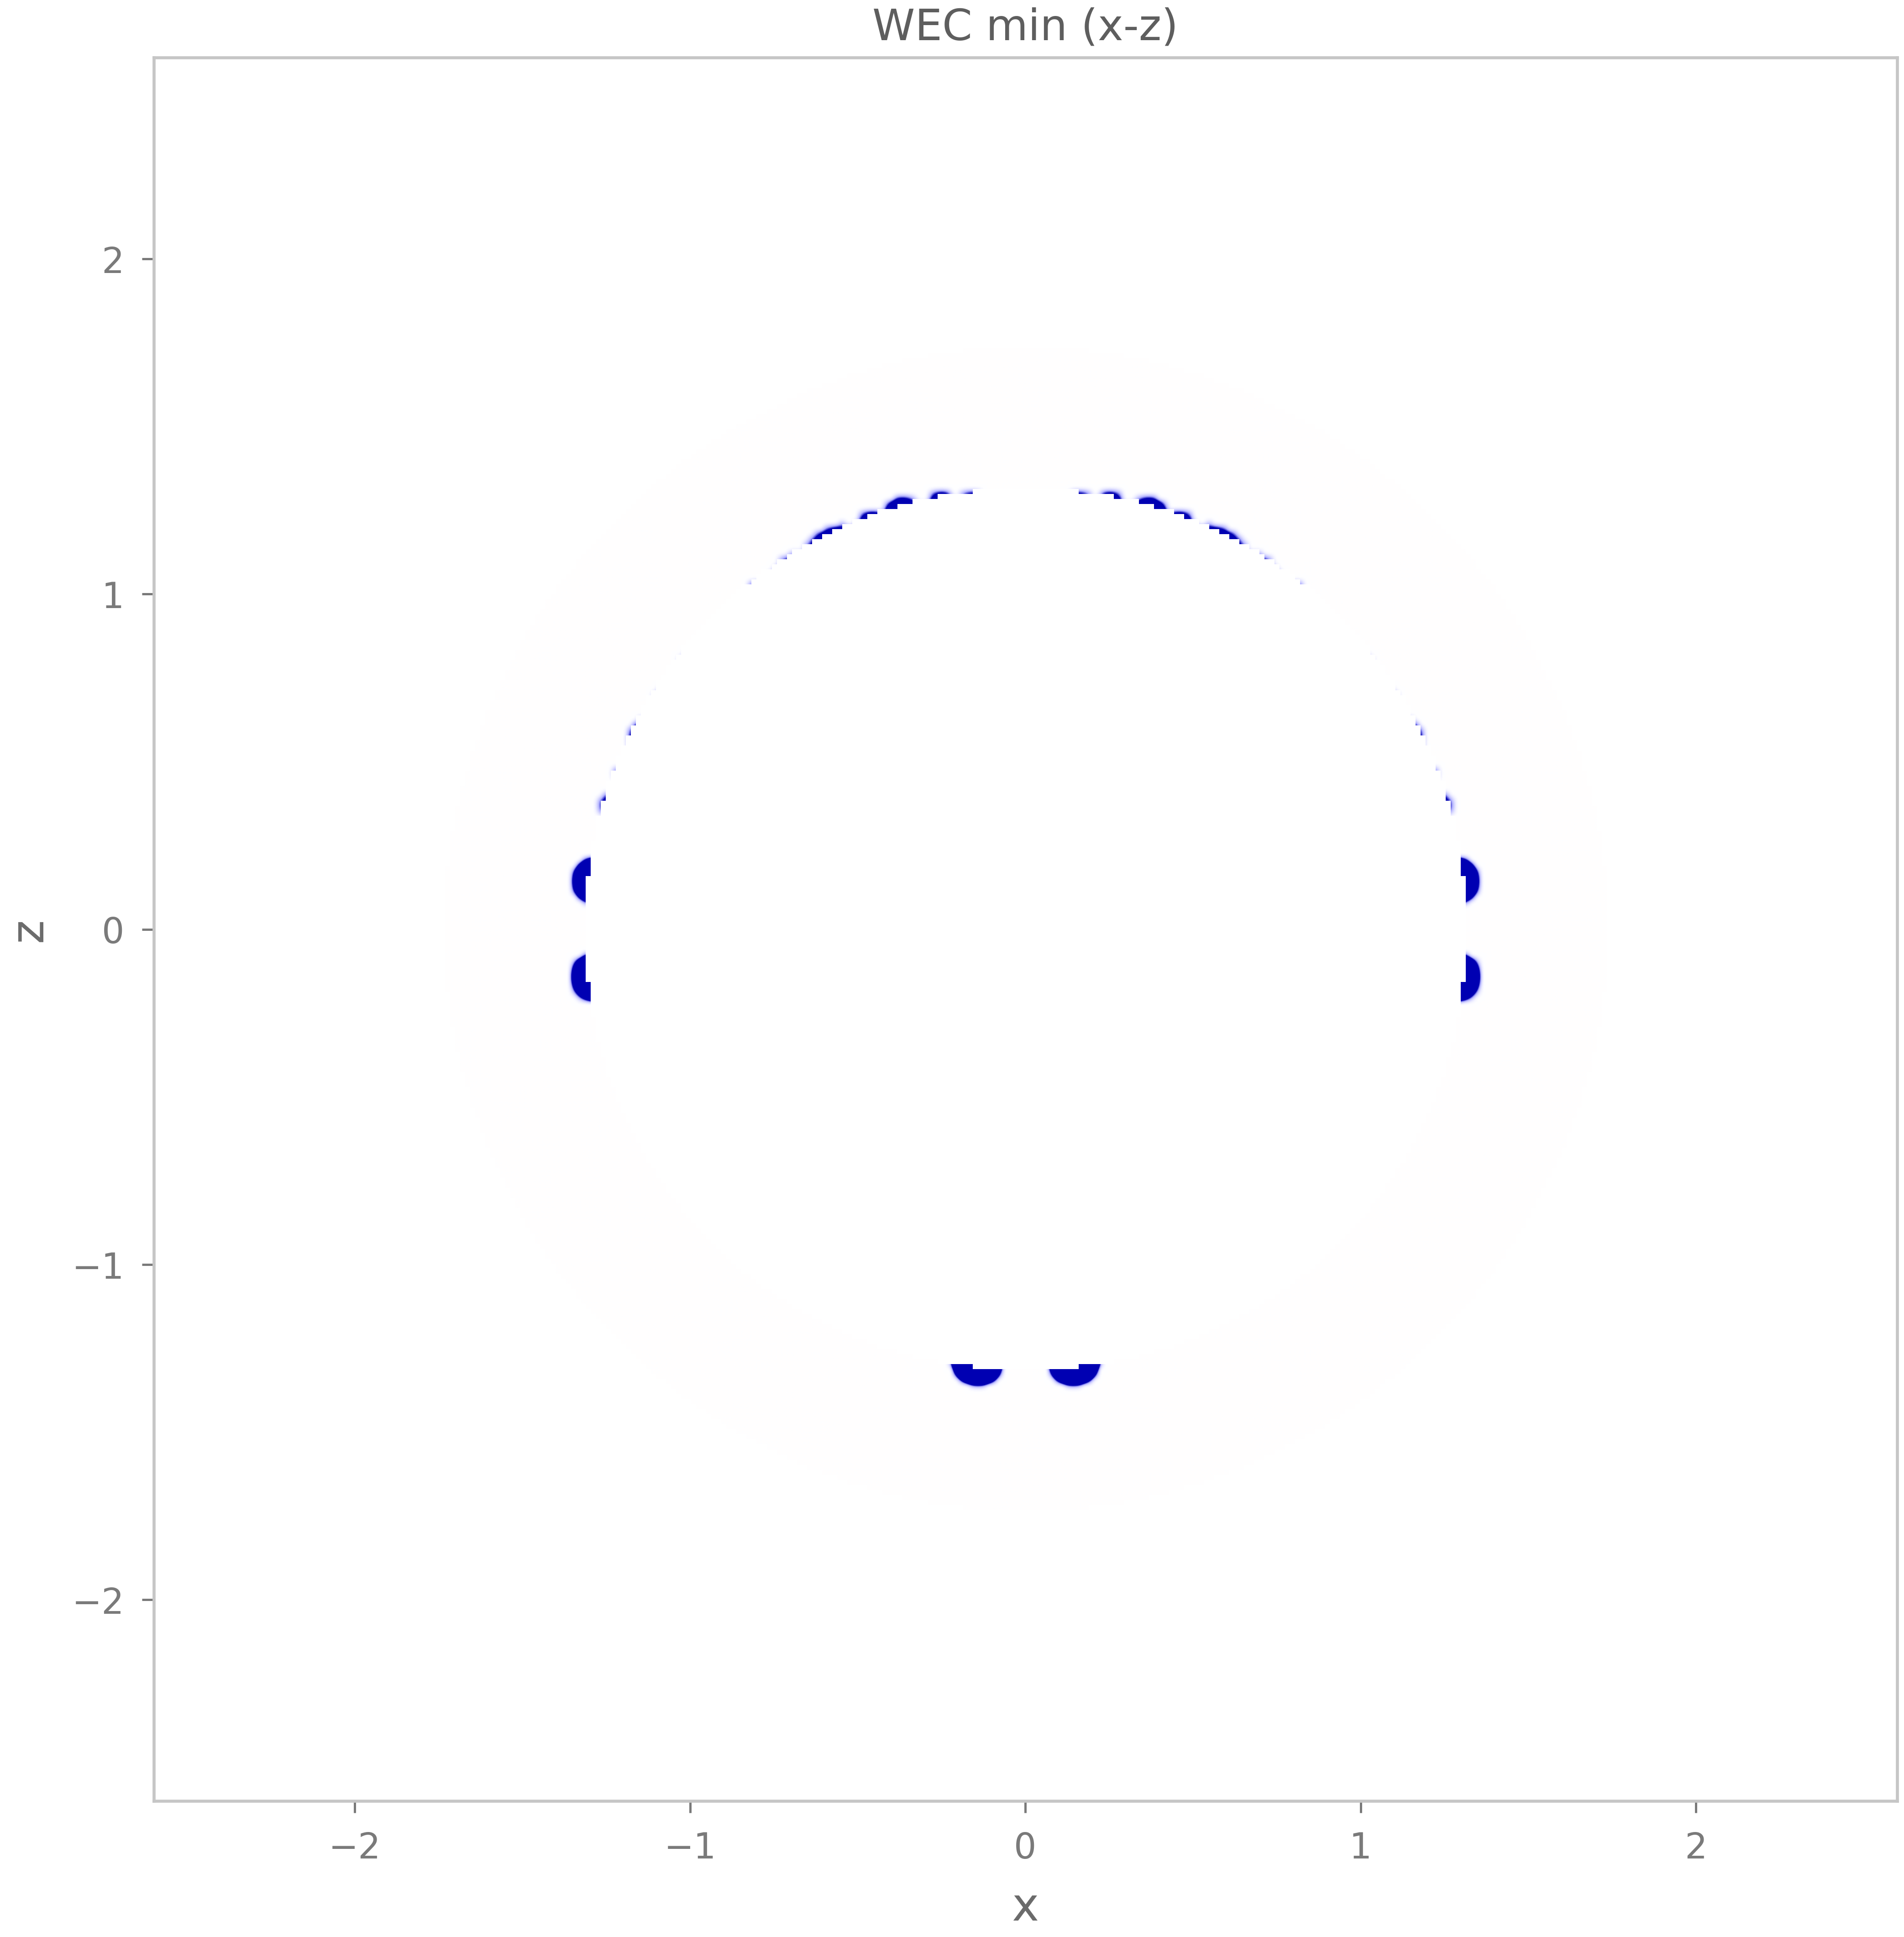
\includegraphics[width=\linewidth]{figures/domain_2_v_0p1_t_30p0_a1p848_b1p135_R01p292_XZ_WECmin.png}
    \caption{\(\mathrm{WEC}_{\min}\) along \(x\mbox{--}z\); violations are localized near the inner interface and slightly elongated along the direction of motion.}
    \label{fig:d2-xz-wecmin}
  \end{subfigure}

  \vspace{1ex}

  \begin{subfigure}[b]{0.46\textwidth}
    \centering
    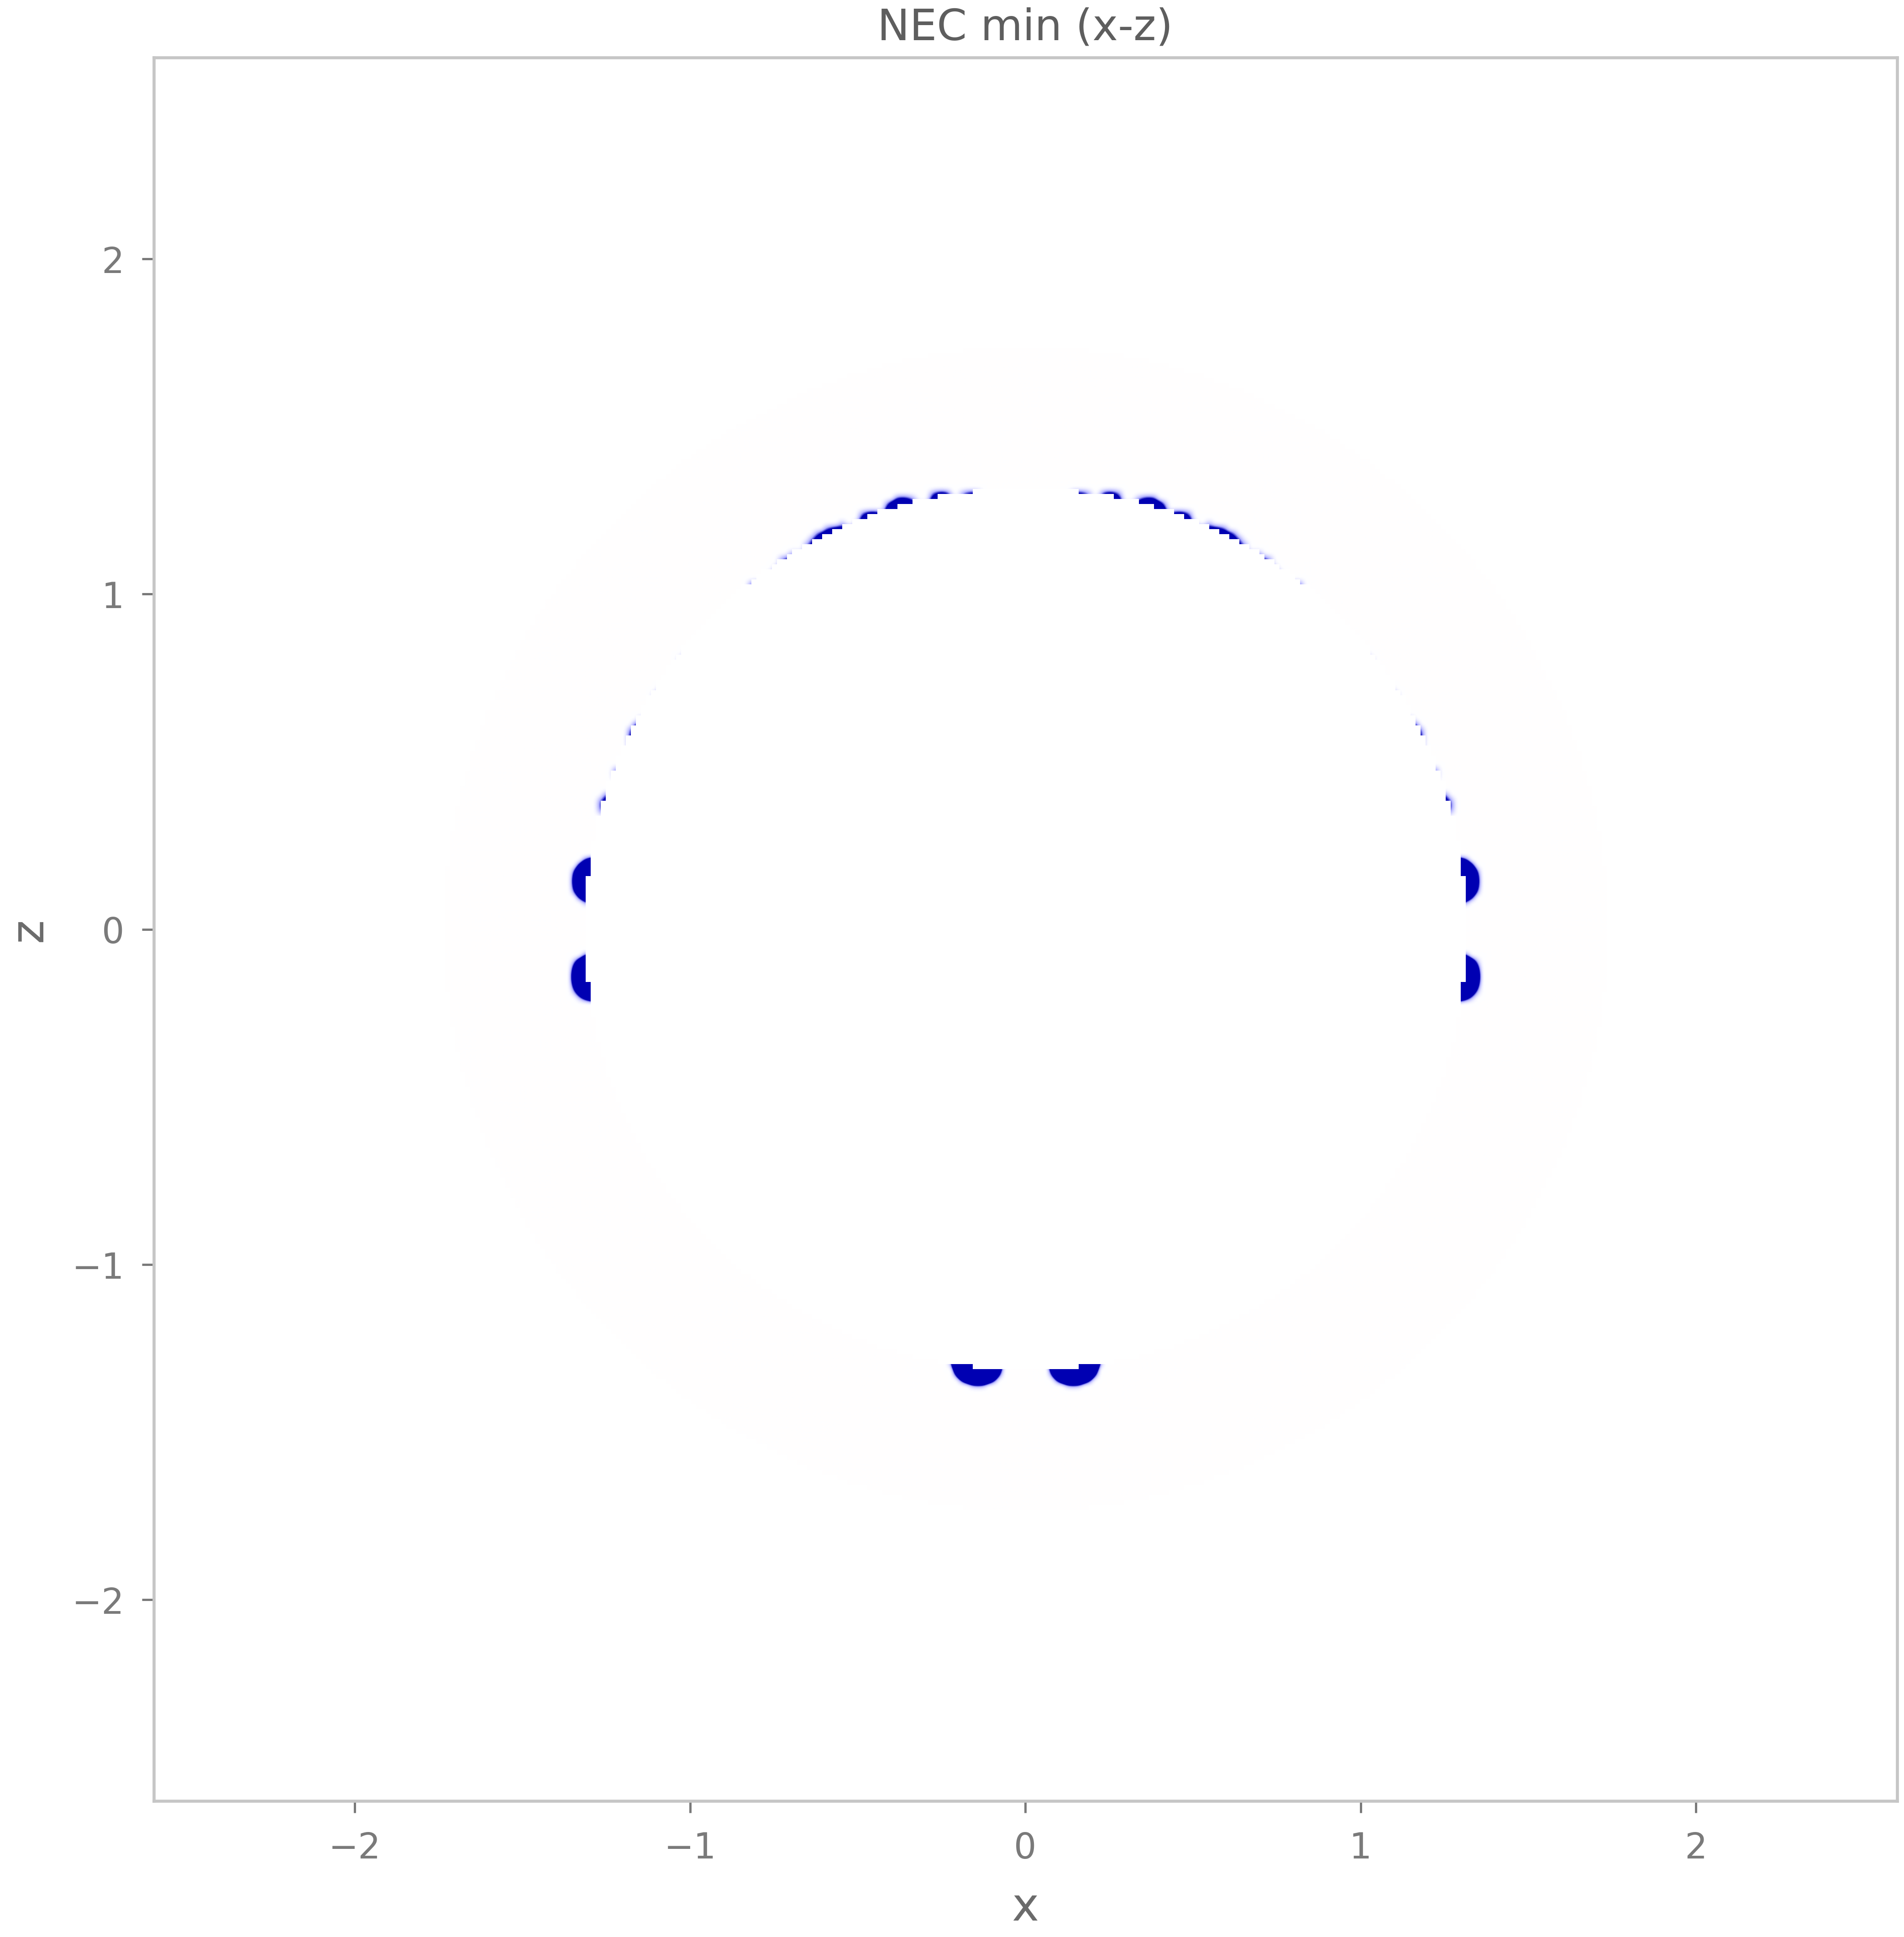
\includegraphics[width=\linewidth]{figures/domain_2_v_0p1_t_30p0_a1p848_b1p135_R01p292_XZ_NECmin.png}
    \caption{\(\mathrm{NEC}_{\min}\) with the same morphology, confirming that the central deficits seen in Fig.~\ref{fig:d2-xy-energy-A} are genuinely three-dimensional.}
    \label{fig:d2-xz-necmin}
  \end{subfigure}

  \caption{Double-shell configuration, meridional \(x\mbox{--}z\) slice:
  density and minimum \WEC/\NEC\ margins, providing the complementary view to Fig.~\ref{fig:d2-xy-energy-A}.}
  \label{fig:d2-xz-energy-A}
\end{figure}

%-----------------------------------------------------
% Double shell: Energy conditions, XZ slice (2 panels)
%-----------------------------------------------------
\begin{figure}[htbp]
  \centering
  \begin{subfigure}[b]{0.46\textwidth}
    \centering
    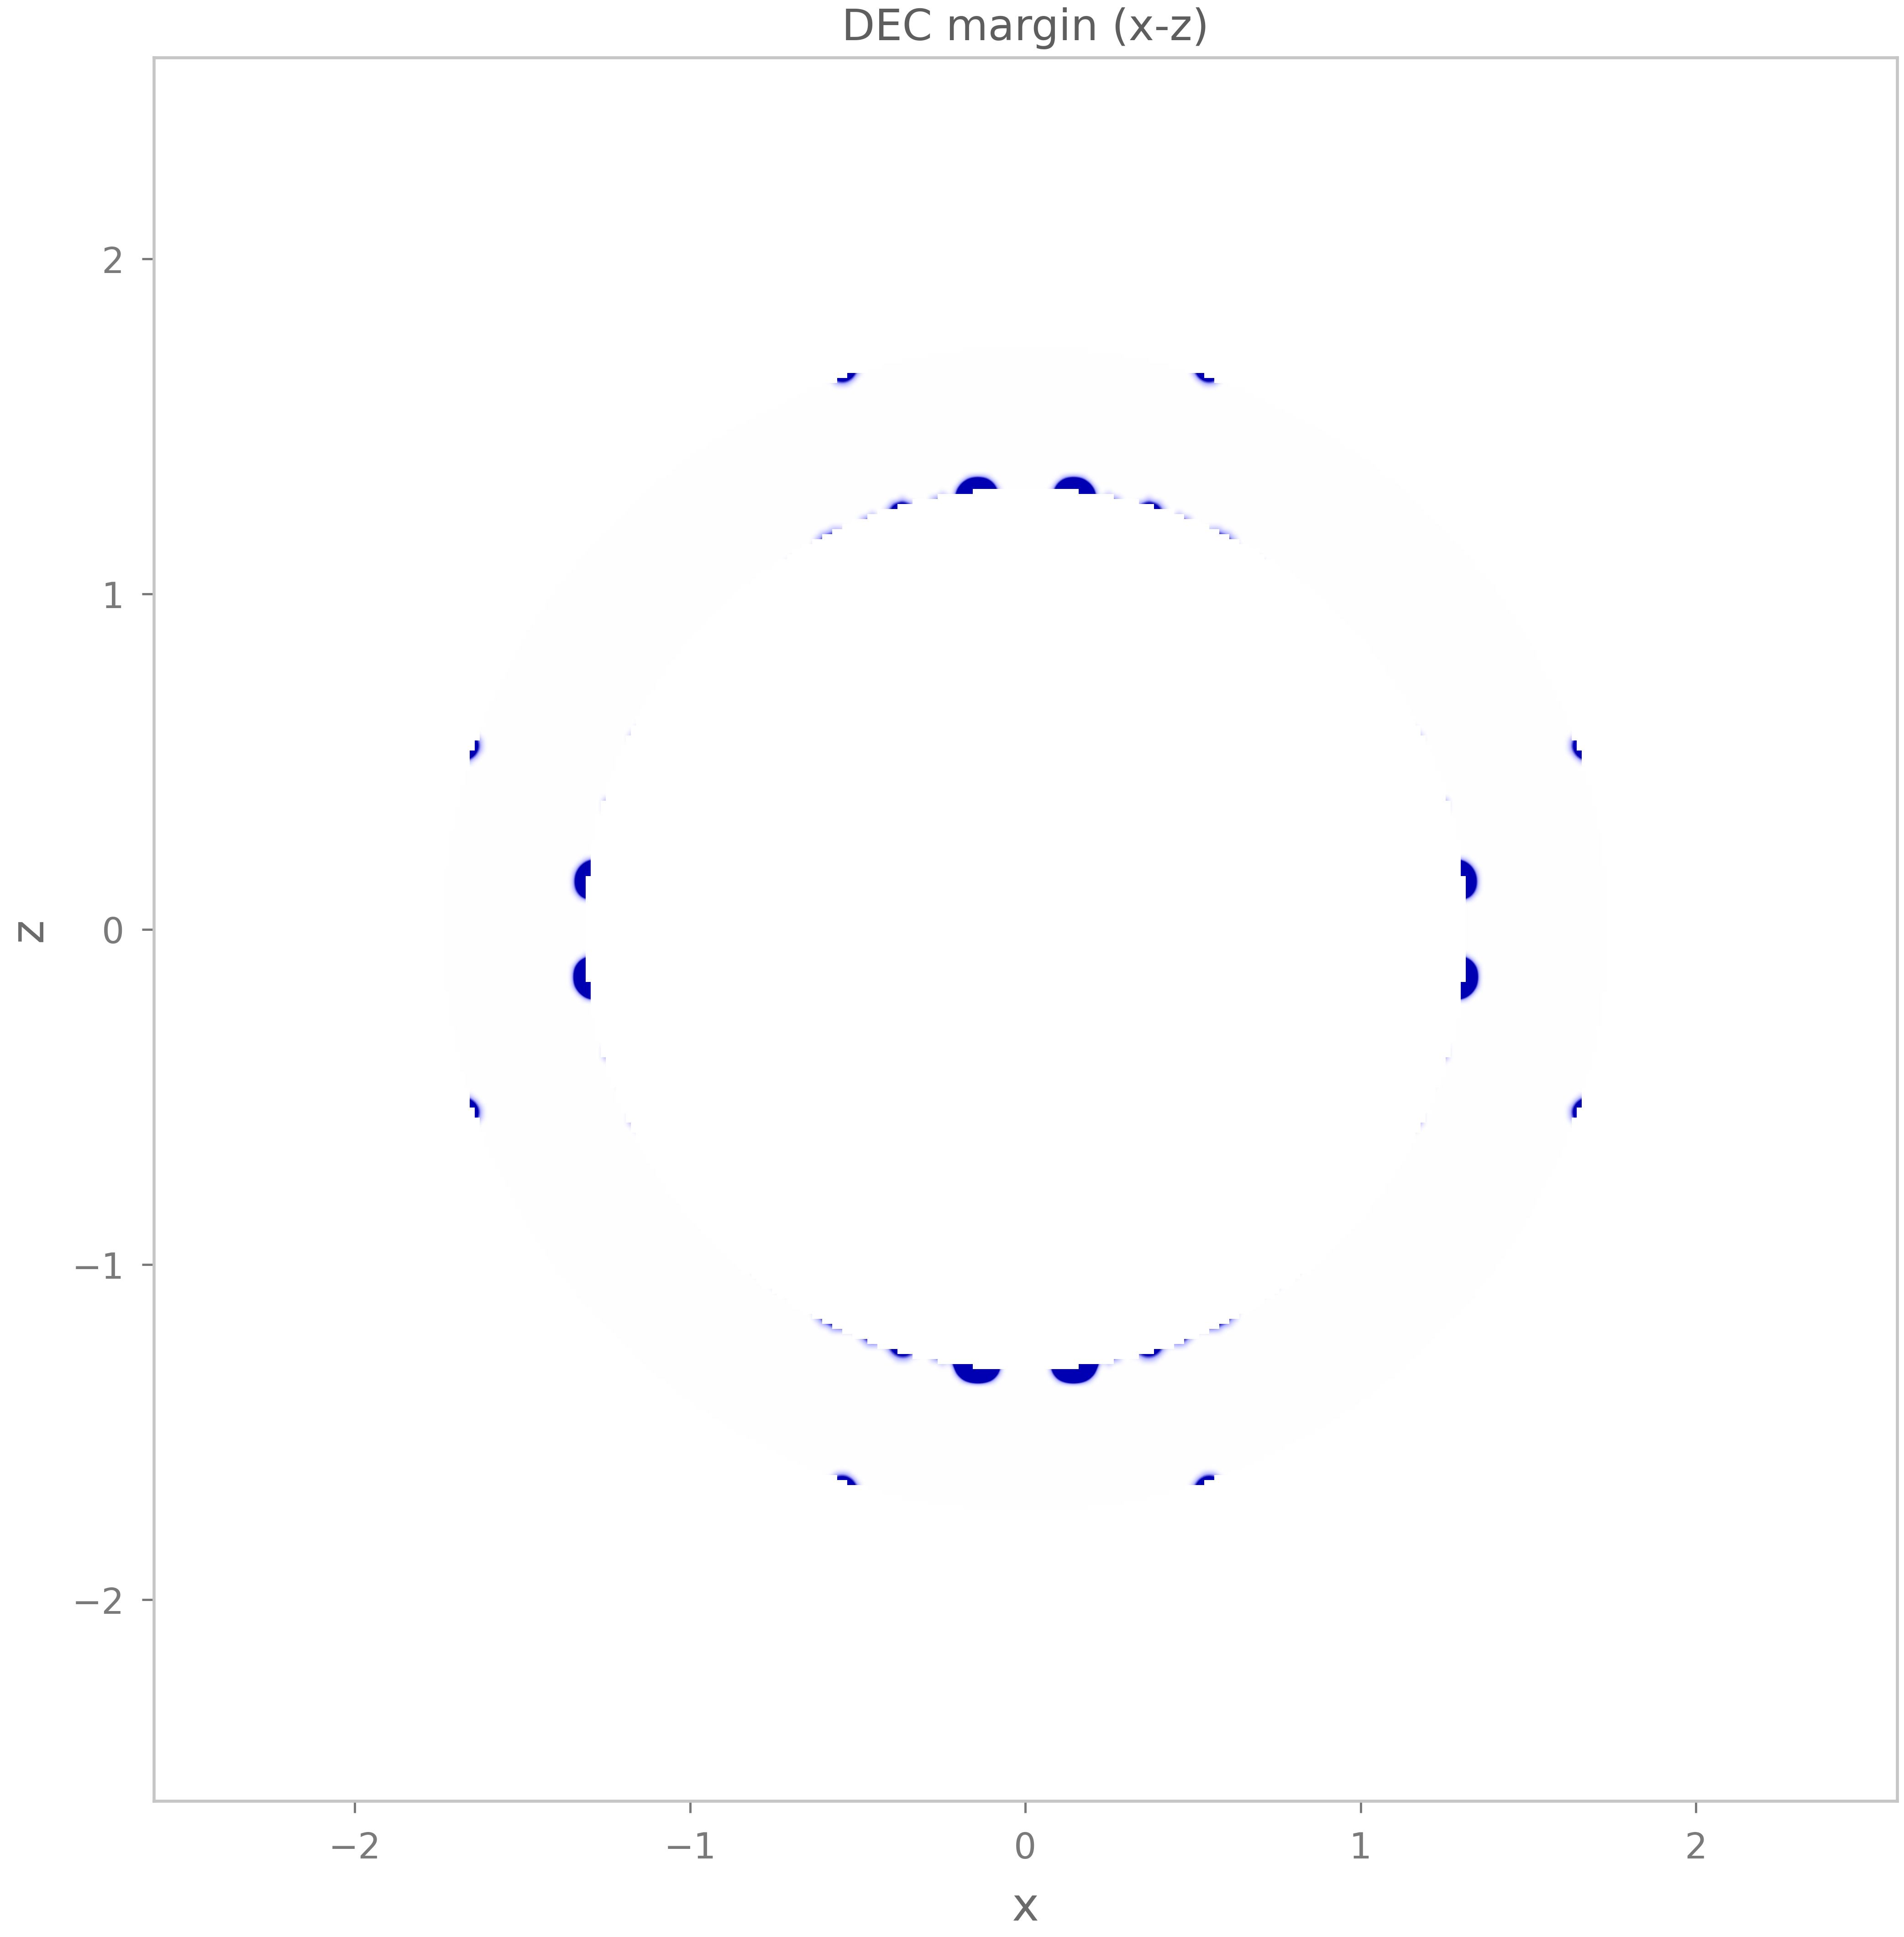
\includegraphics[width=\linewidth]{figures/domain_2_v_0p1_t_30p0_a1p848_b1p135_R01p292_XZ_DECmargin.png}
    \caption{DEC margin on the meridional slice, showing how tangential-stress excess spreads slightly along the equatorial plane but remains tied to the interfaces.}
    \label{fig:d2-xz-decmargin}
  \end{subfigure}\hfill
  \begin{subfigure}[b]{0.46\textwidth}
    \centering
    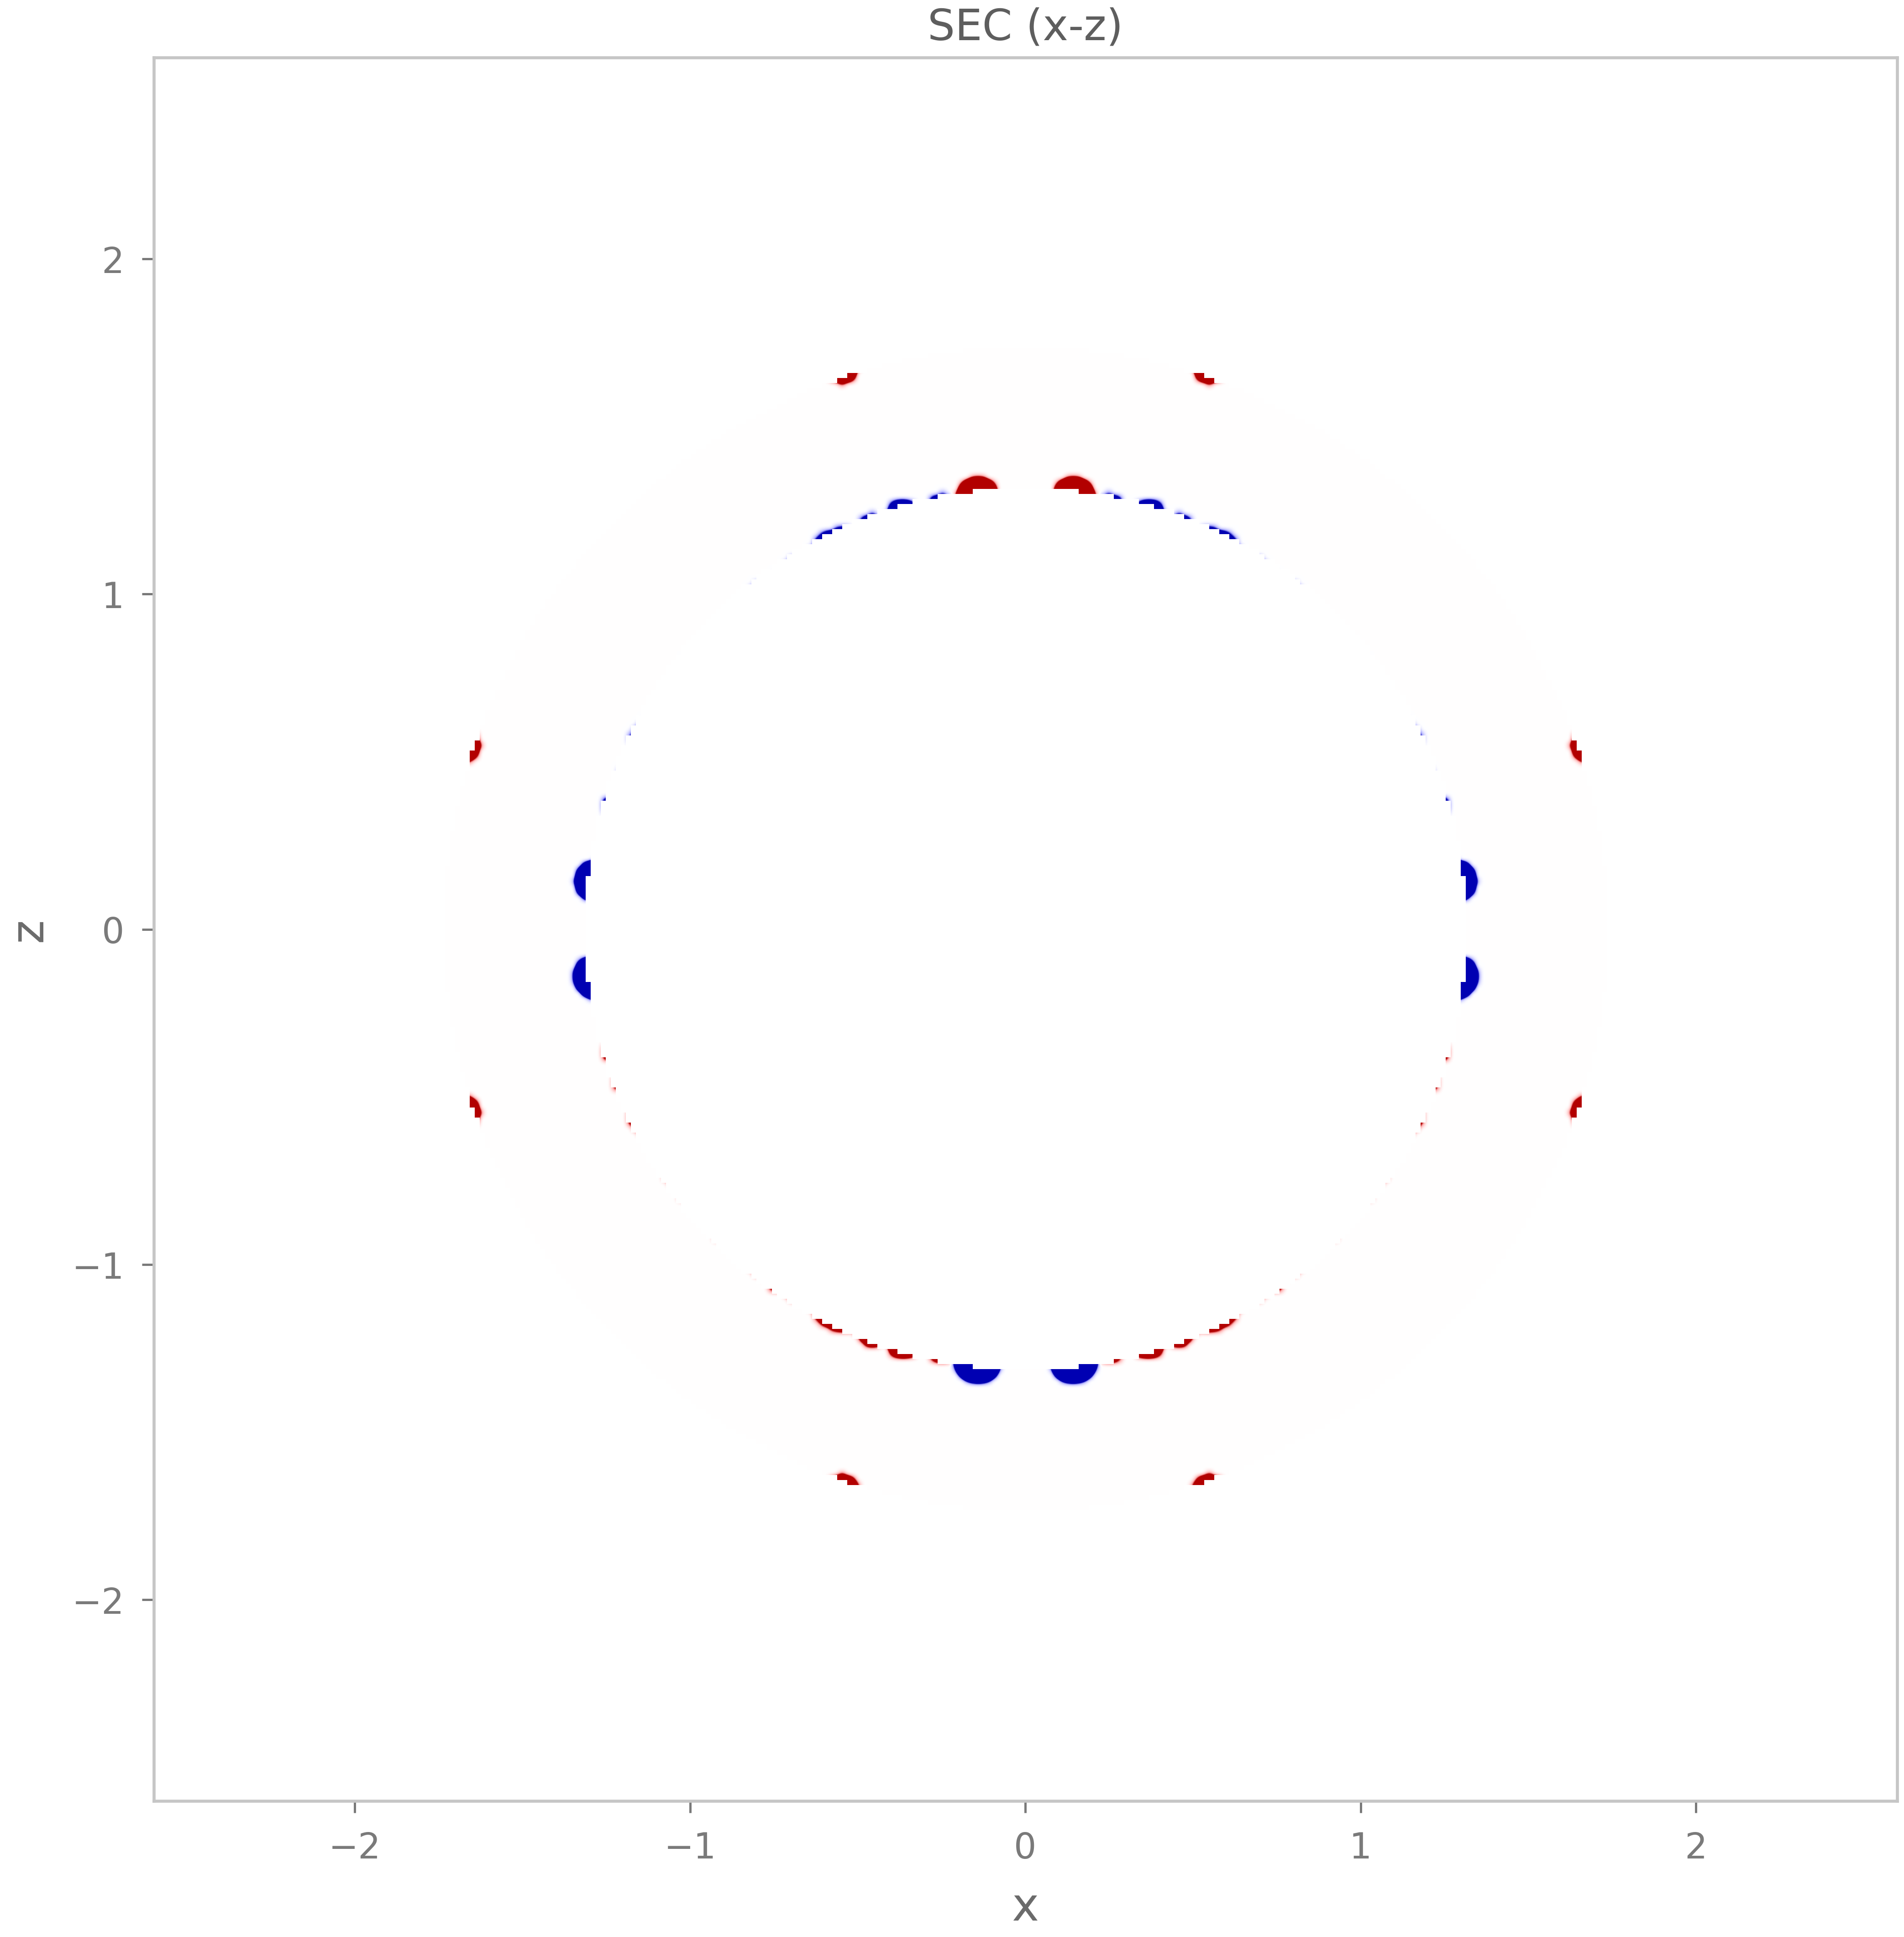
\includegraphics[width=\linewidth]{figures/domain_2_v_0p1_t_30p0_a1p848_b1p135_R01p292_XZ_SEC.png}
    \caption{\(\SEC\) on the same slice; the pattern is sign-changing but remains less restrictive in aggregate than the \DEC, consistent with the higher final SEC success fraction.}
    \label{fig:d2-xz-sec}
  \end{subfigure}

  \caption{Double-shell configuration, meridional slice:
  \DEC\ and \SEC\ diagnostics, completing the three-dimensional picture of stress localization.}
  \label{fig:d2-xz-energy-B}
\end{figure}

%-----------------------------------------------------
% Single shell: Optimization diagnostics
%-----------------------------------------------------
\begin{figure}[p]
  \centering

  \begin{subfigure}[t]{0.47\textwidth}
    \centering
    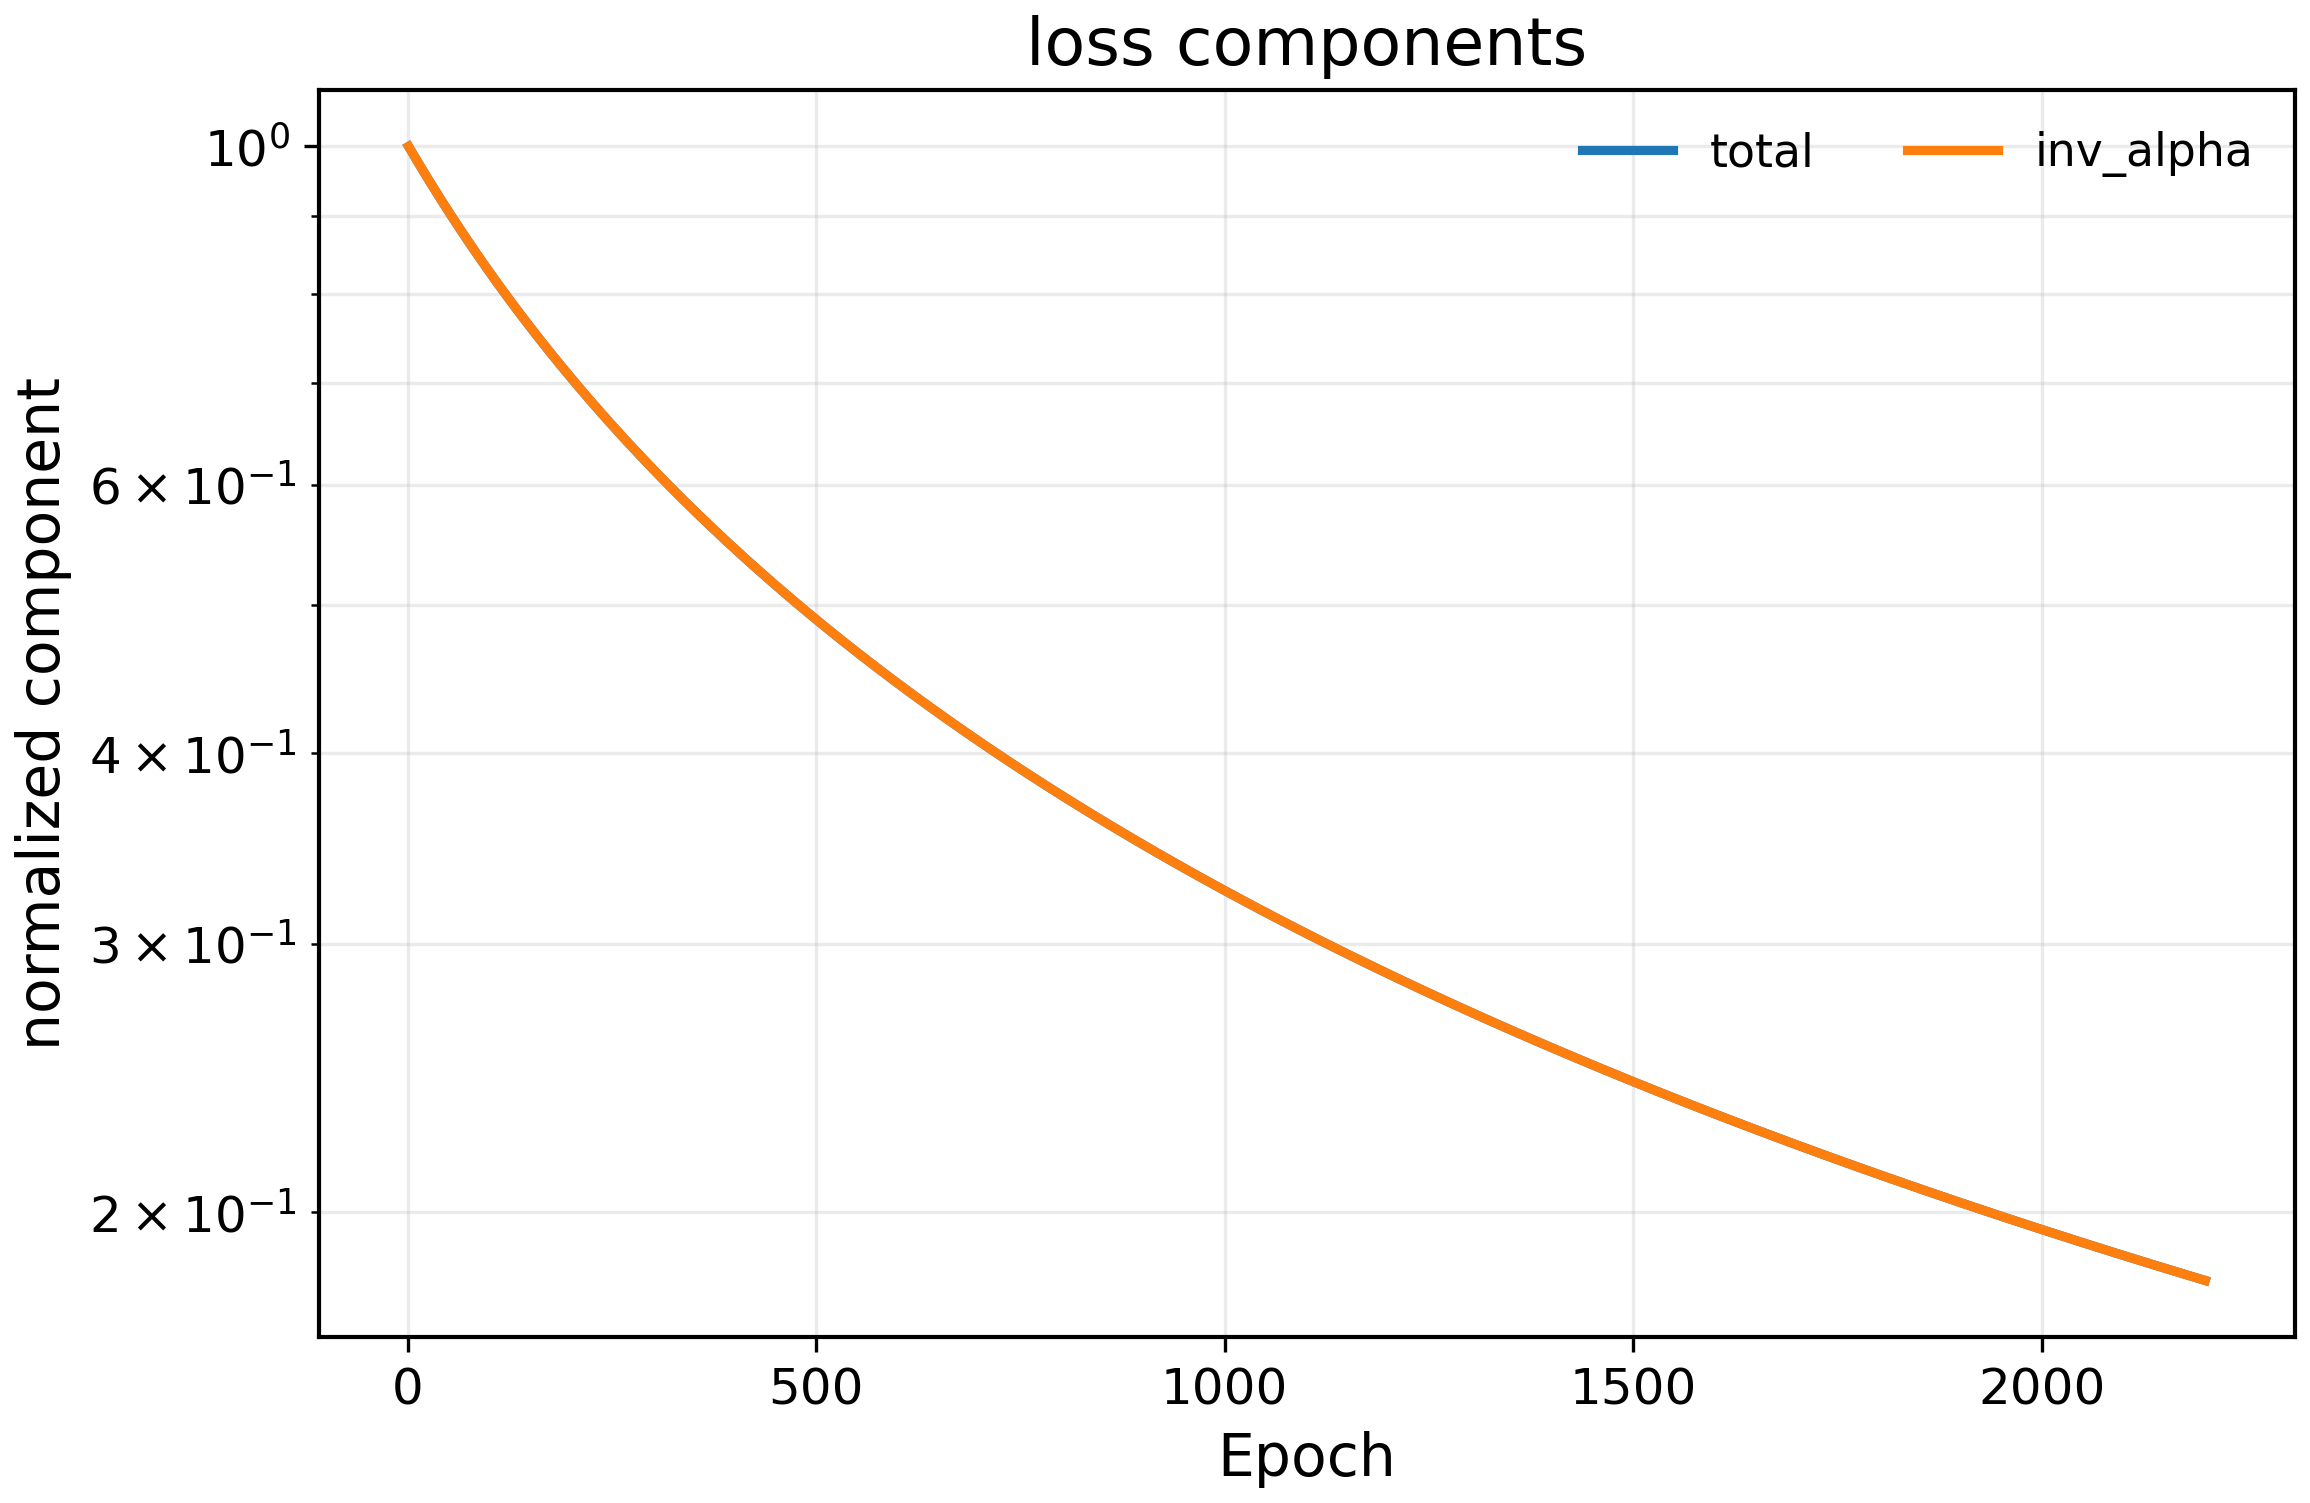
\includegraphics[width=\linewidth]{figures/domain_1_v_0p1_t_30p0_loss_components.png}
    \caption{Loss components across epochs.}
    \label{fig:d1-loss-components}
  \end{subfigure}\hfill
  \begin{subfigure}[t]{0.47\textwidth}
    \centering
    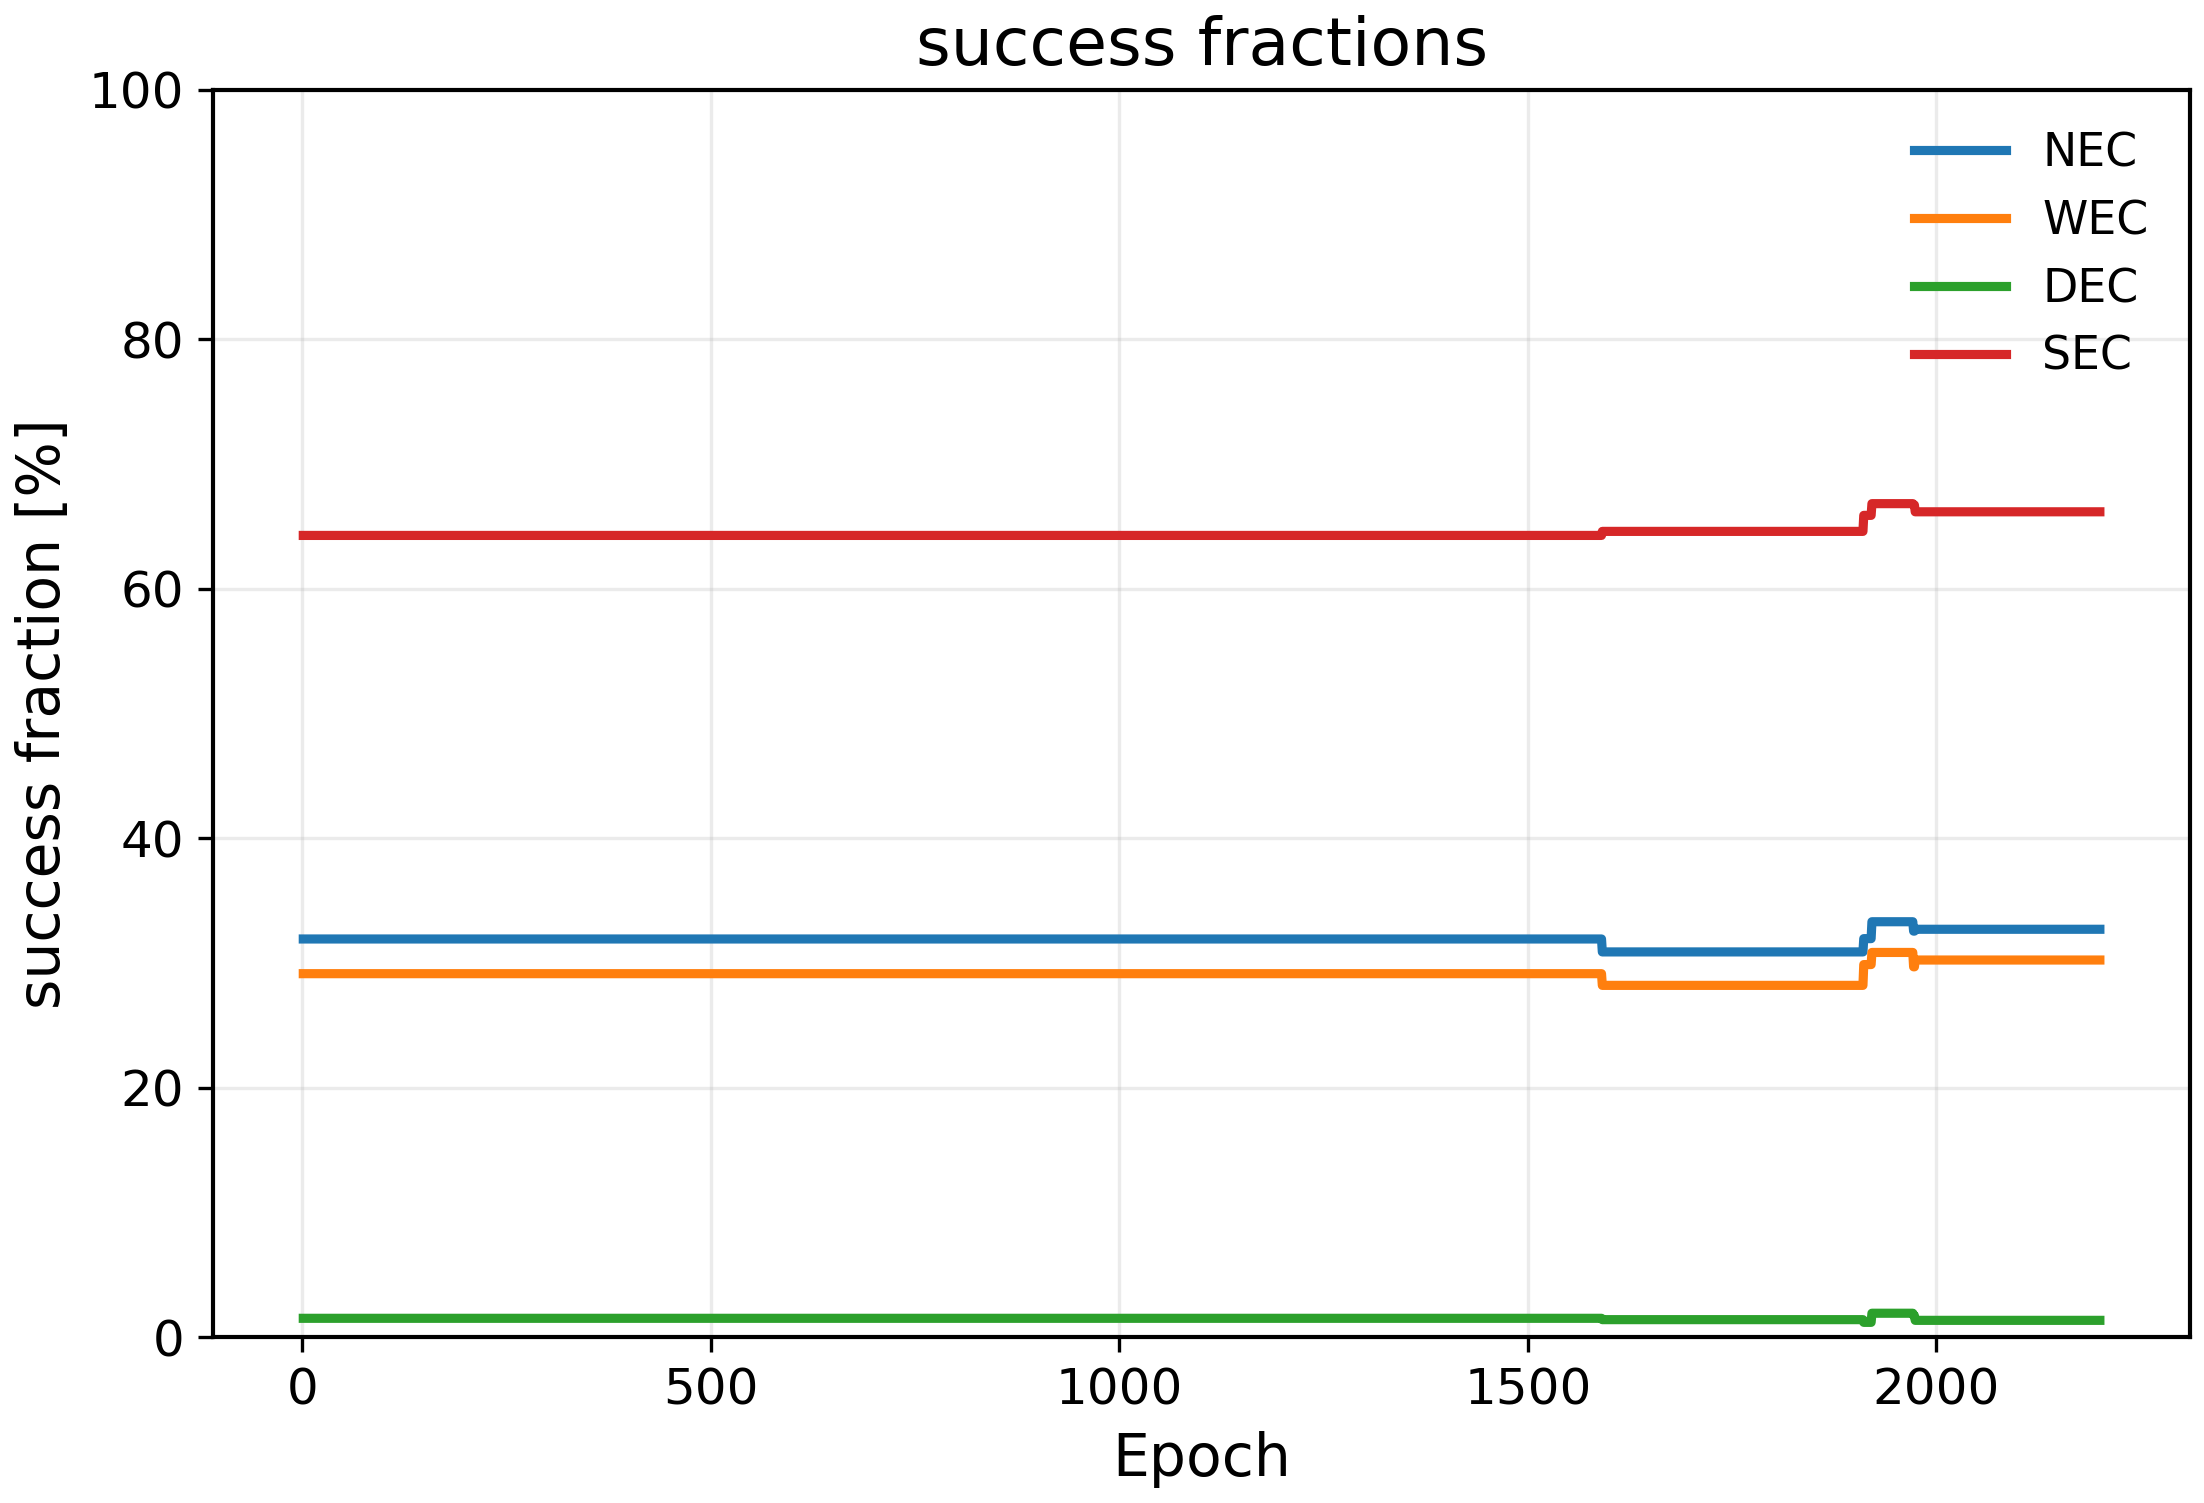
\includegraphics[width=\linewidth]{figures/domain_1_v_0p1_t_30p0_success_fractions.png}
    \caption{Success fractions for NEC/WEC/DEC/SEC.}
    \label{fig:d1-success}
  \end{subfigure}

  \vspace{1ex}

  \begin{subfigure}[t]{0.62\textwidth}
    \centering
    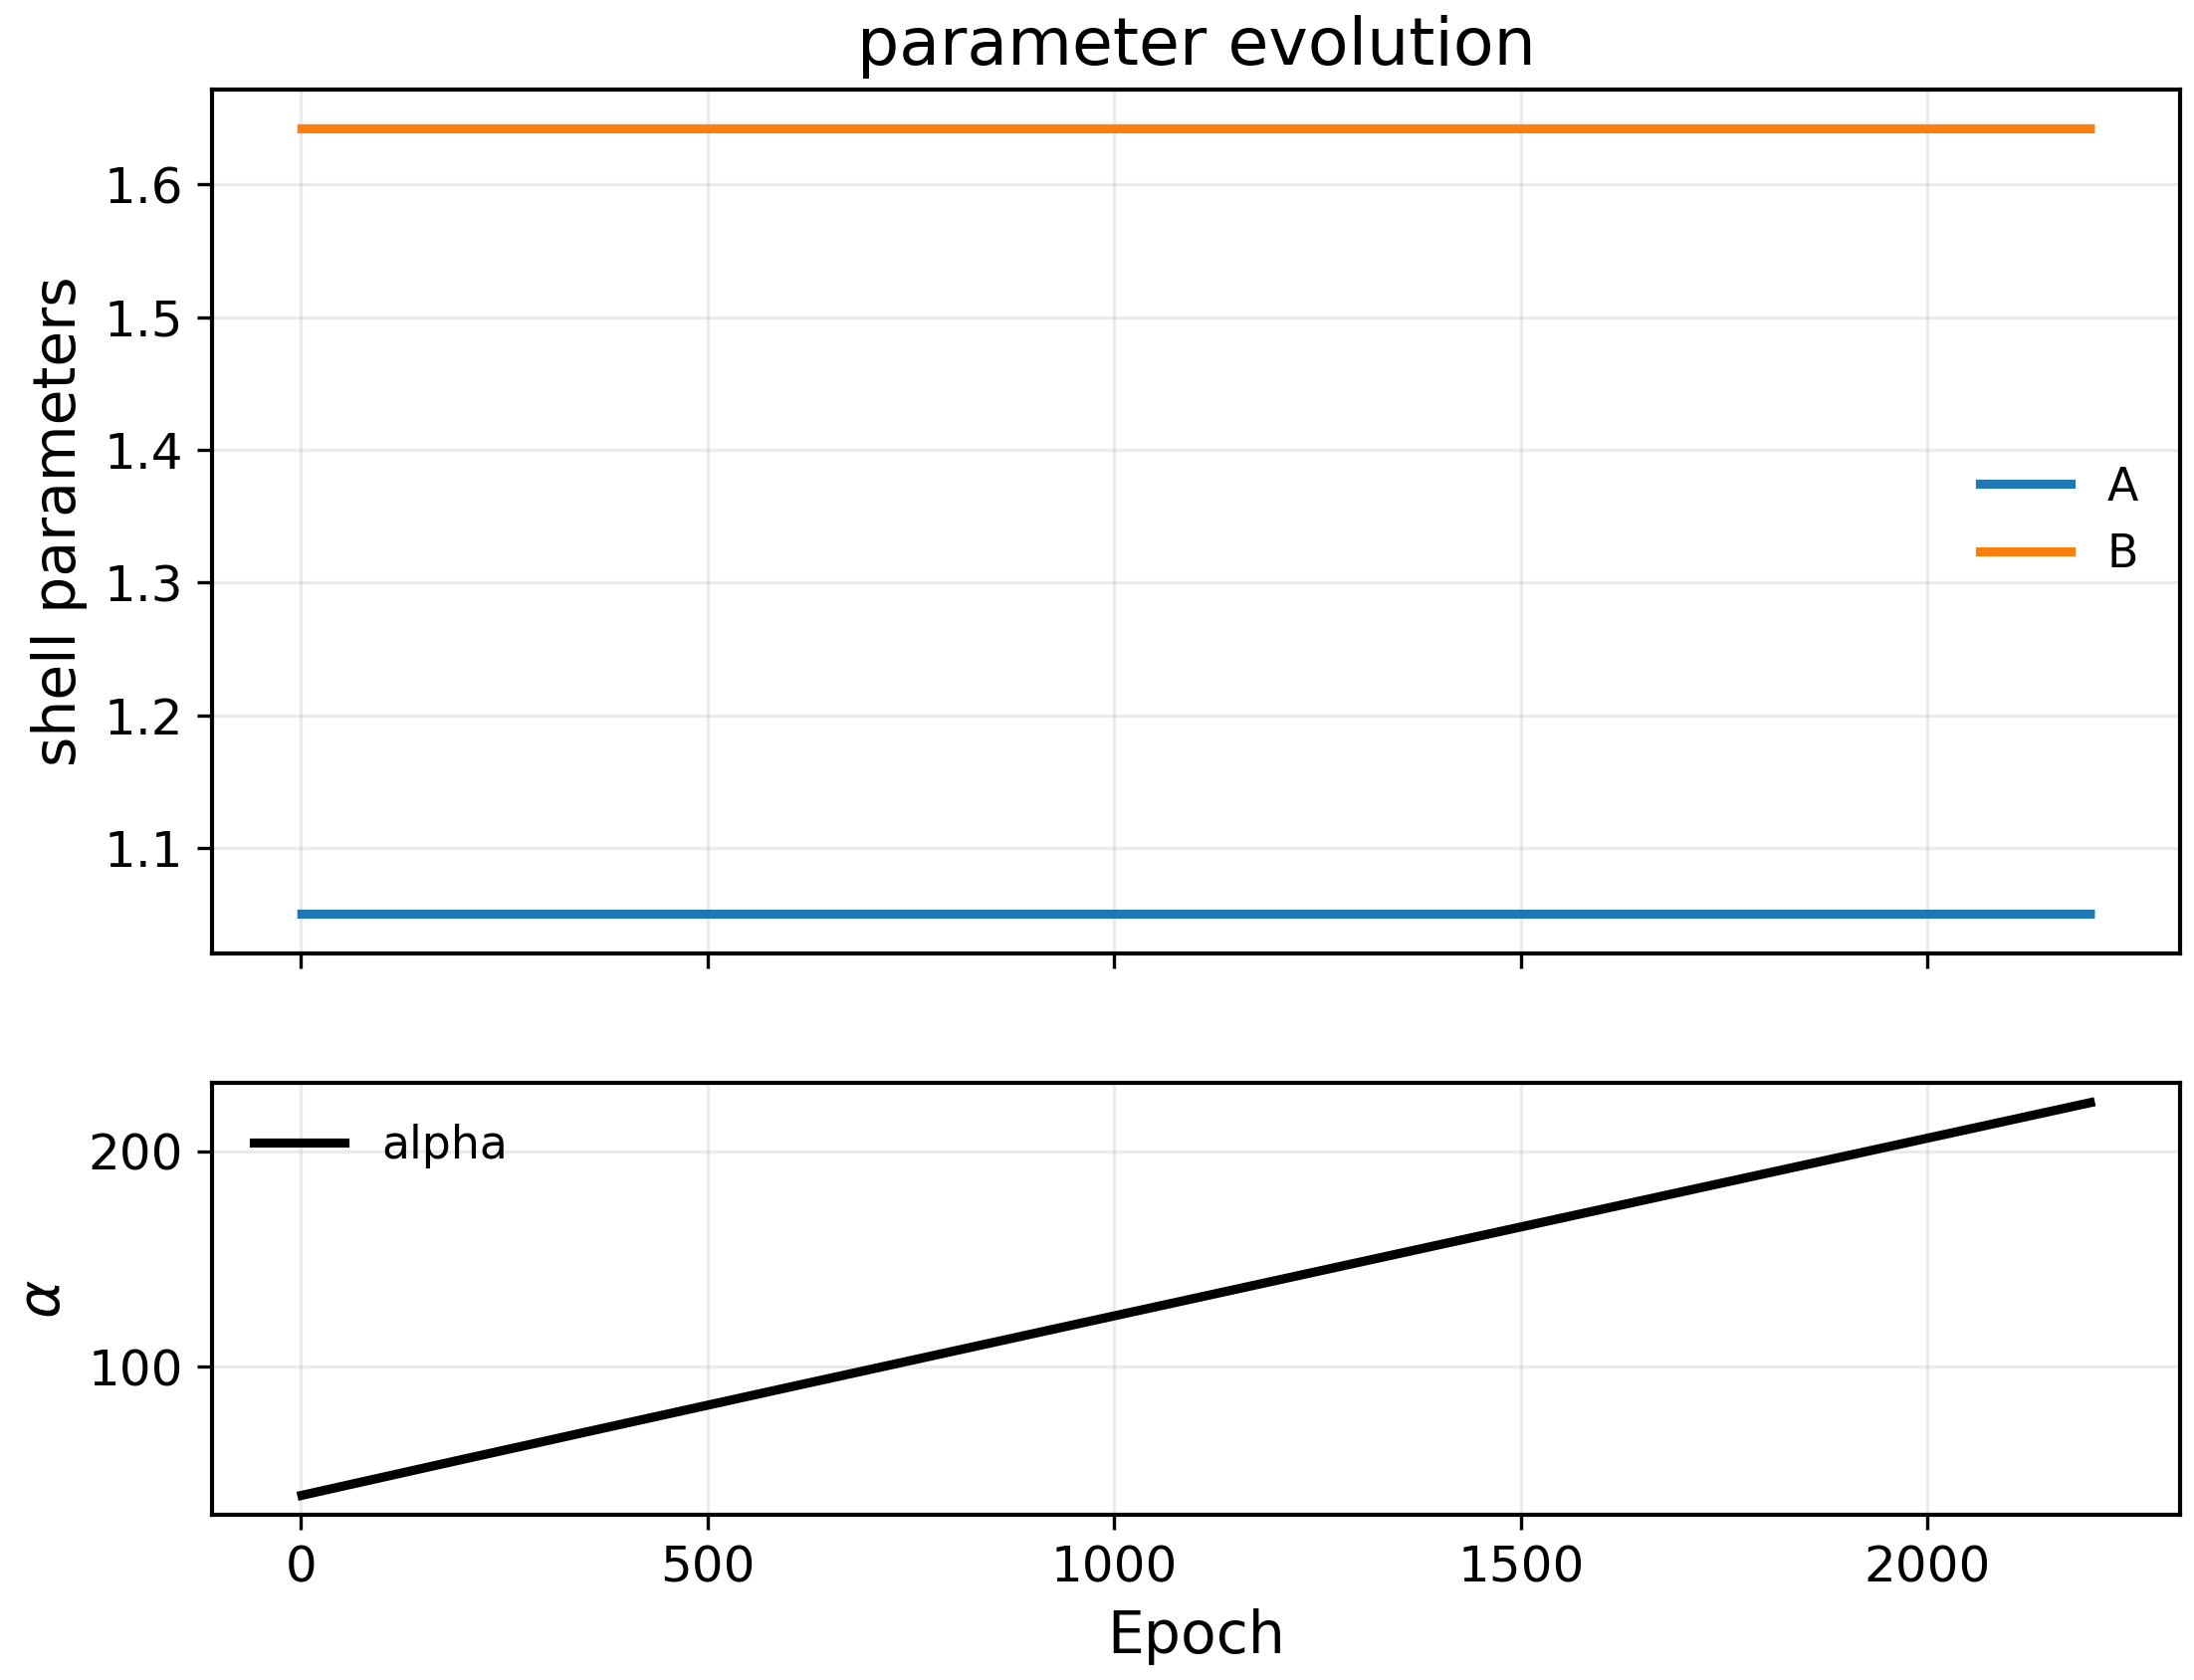
\includegraphics[width=\linewidth]{figures/domain_1_v_0p1_t_30p0_params.png}
    \caption{Seed parameters $A$ and $B$ across epochs.}
    \label{fig:d1-params-epoch}
  \end{subfigure}

  \caption{Optimization diagnostics for the single-shell configuration at $v=0.1$, $t=30$. Panel (a) shows the normalized loss terms \texttt{inv\_alpha}, \texttt{physics\_loss}, \texttt{reg\_breach}, and \texttt{total\_loss}. Panel (b) reports the fractions of grid points satisfying NEC/WEC/DEC/SEC; SEC remains the easiest condition to satisfy, DEC remains the tightest global constraint, and NEC/WEC settle at intermediate but still significantly constrained levels. Panel (c) shows that the main run remains almost stationary in $A$ and $B$, consistent with a pretraining stage that already selected a near-plateau configuration before the published optimization history begins.}

  \label{fig:d1-opt}
\end{figure}

%-----------------------------------------------------
% Double shell: Optimization diagnostics
%-----------------------------------------------------
\begin{figure}[p]
  \centering

  \begin{subfigure}[t]{0.47\textwidth}
    \centering
    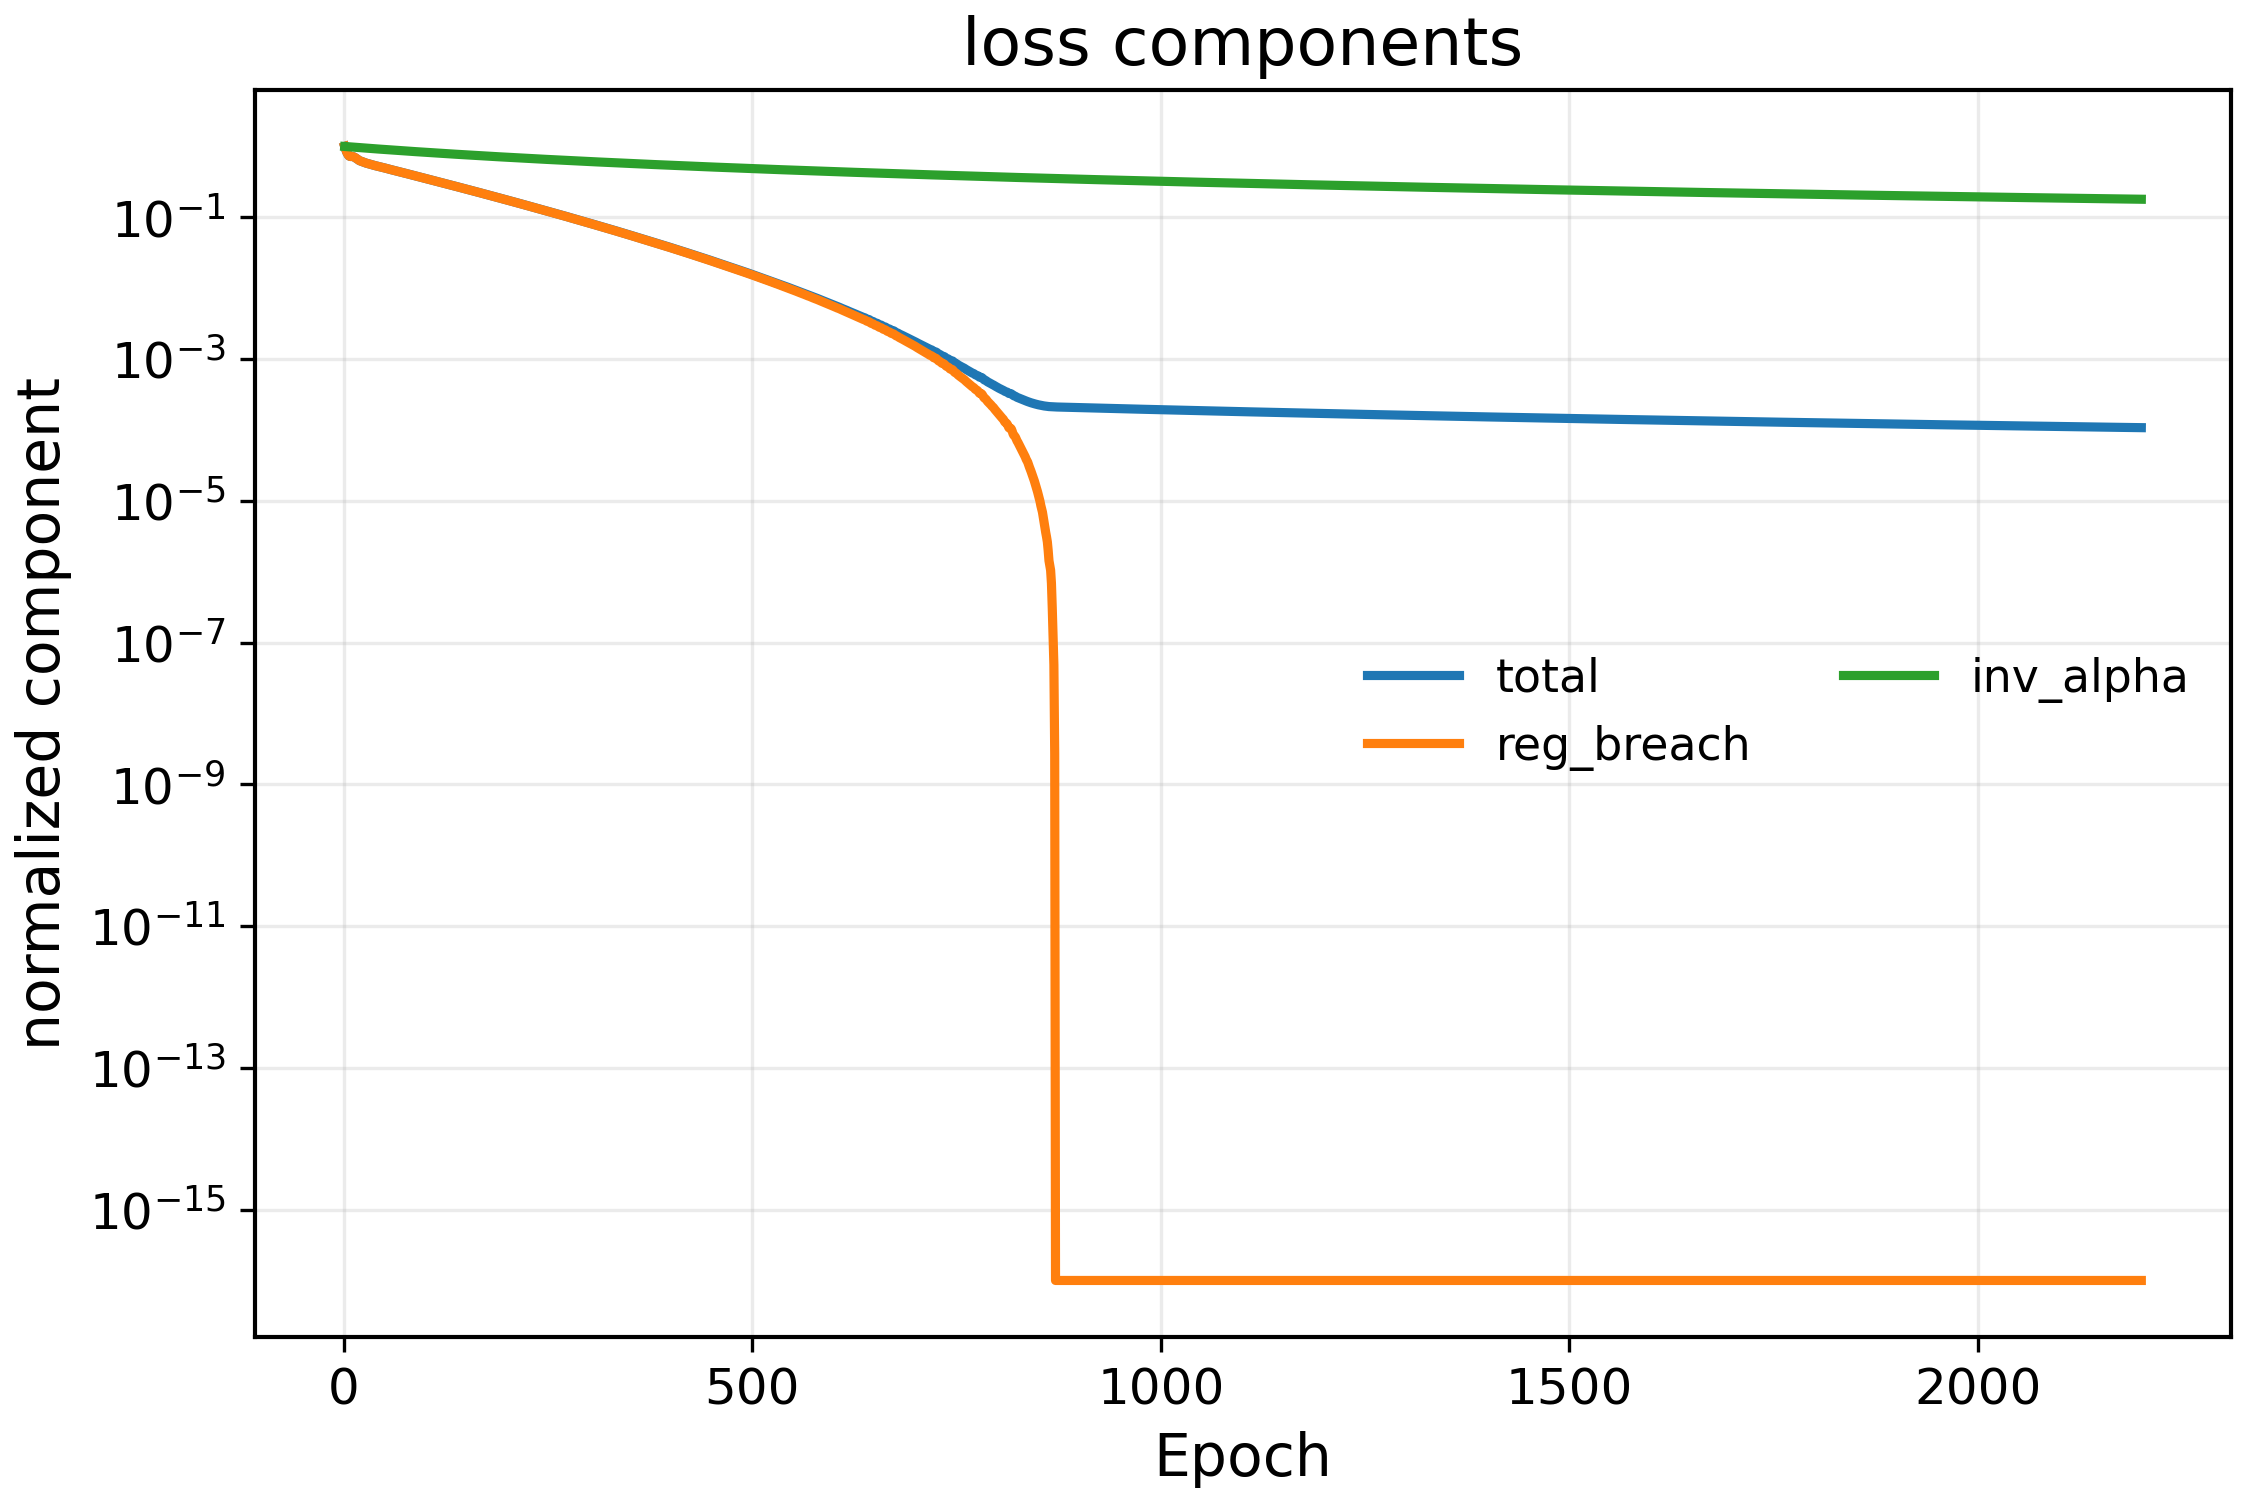
\includegraphics[width=\linewidth]{figures/domain_2_v_0p1_t_30p0_loss_components.png}
    \caption{Loss components across epochs.}
    \label{fig:d2-loss-components}
  \end{subfigure}\hfill
  \begin{subfigure}[t]{0.47\textwidth}
    \centering
    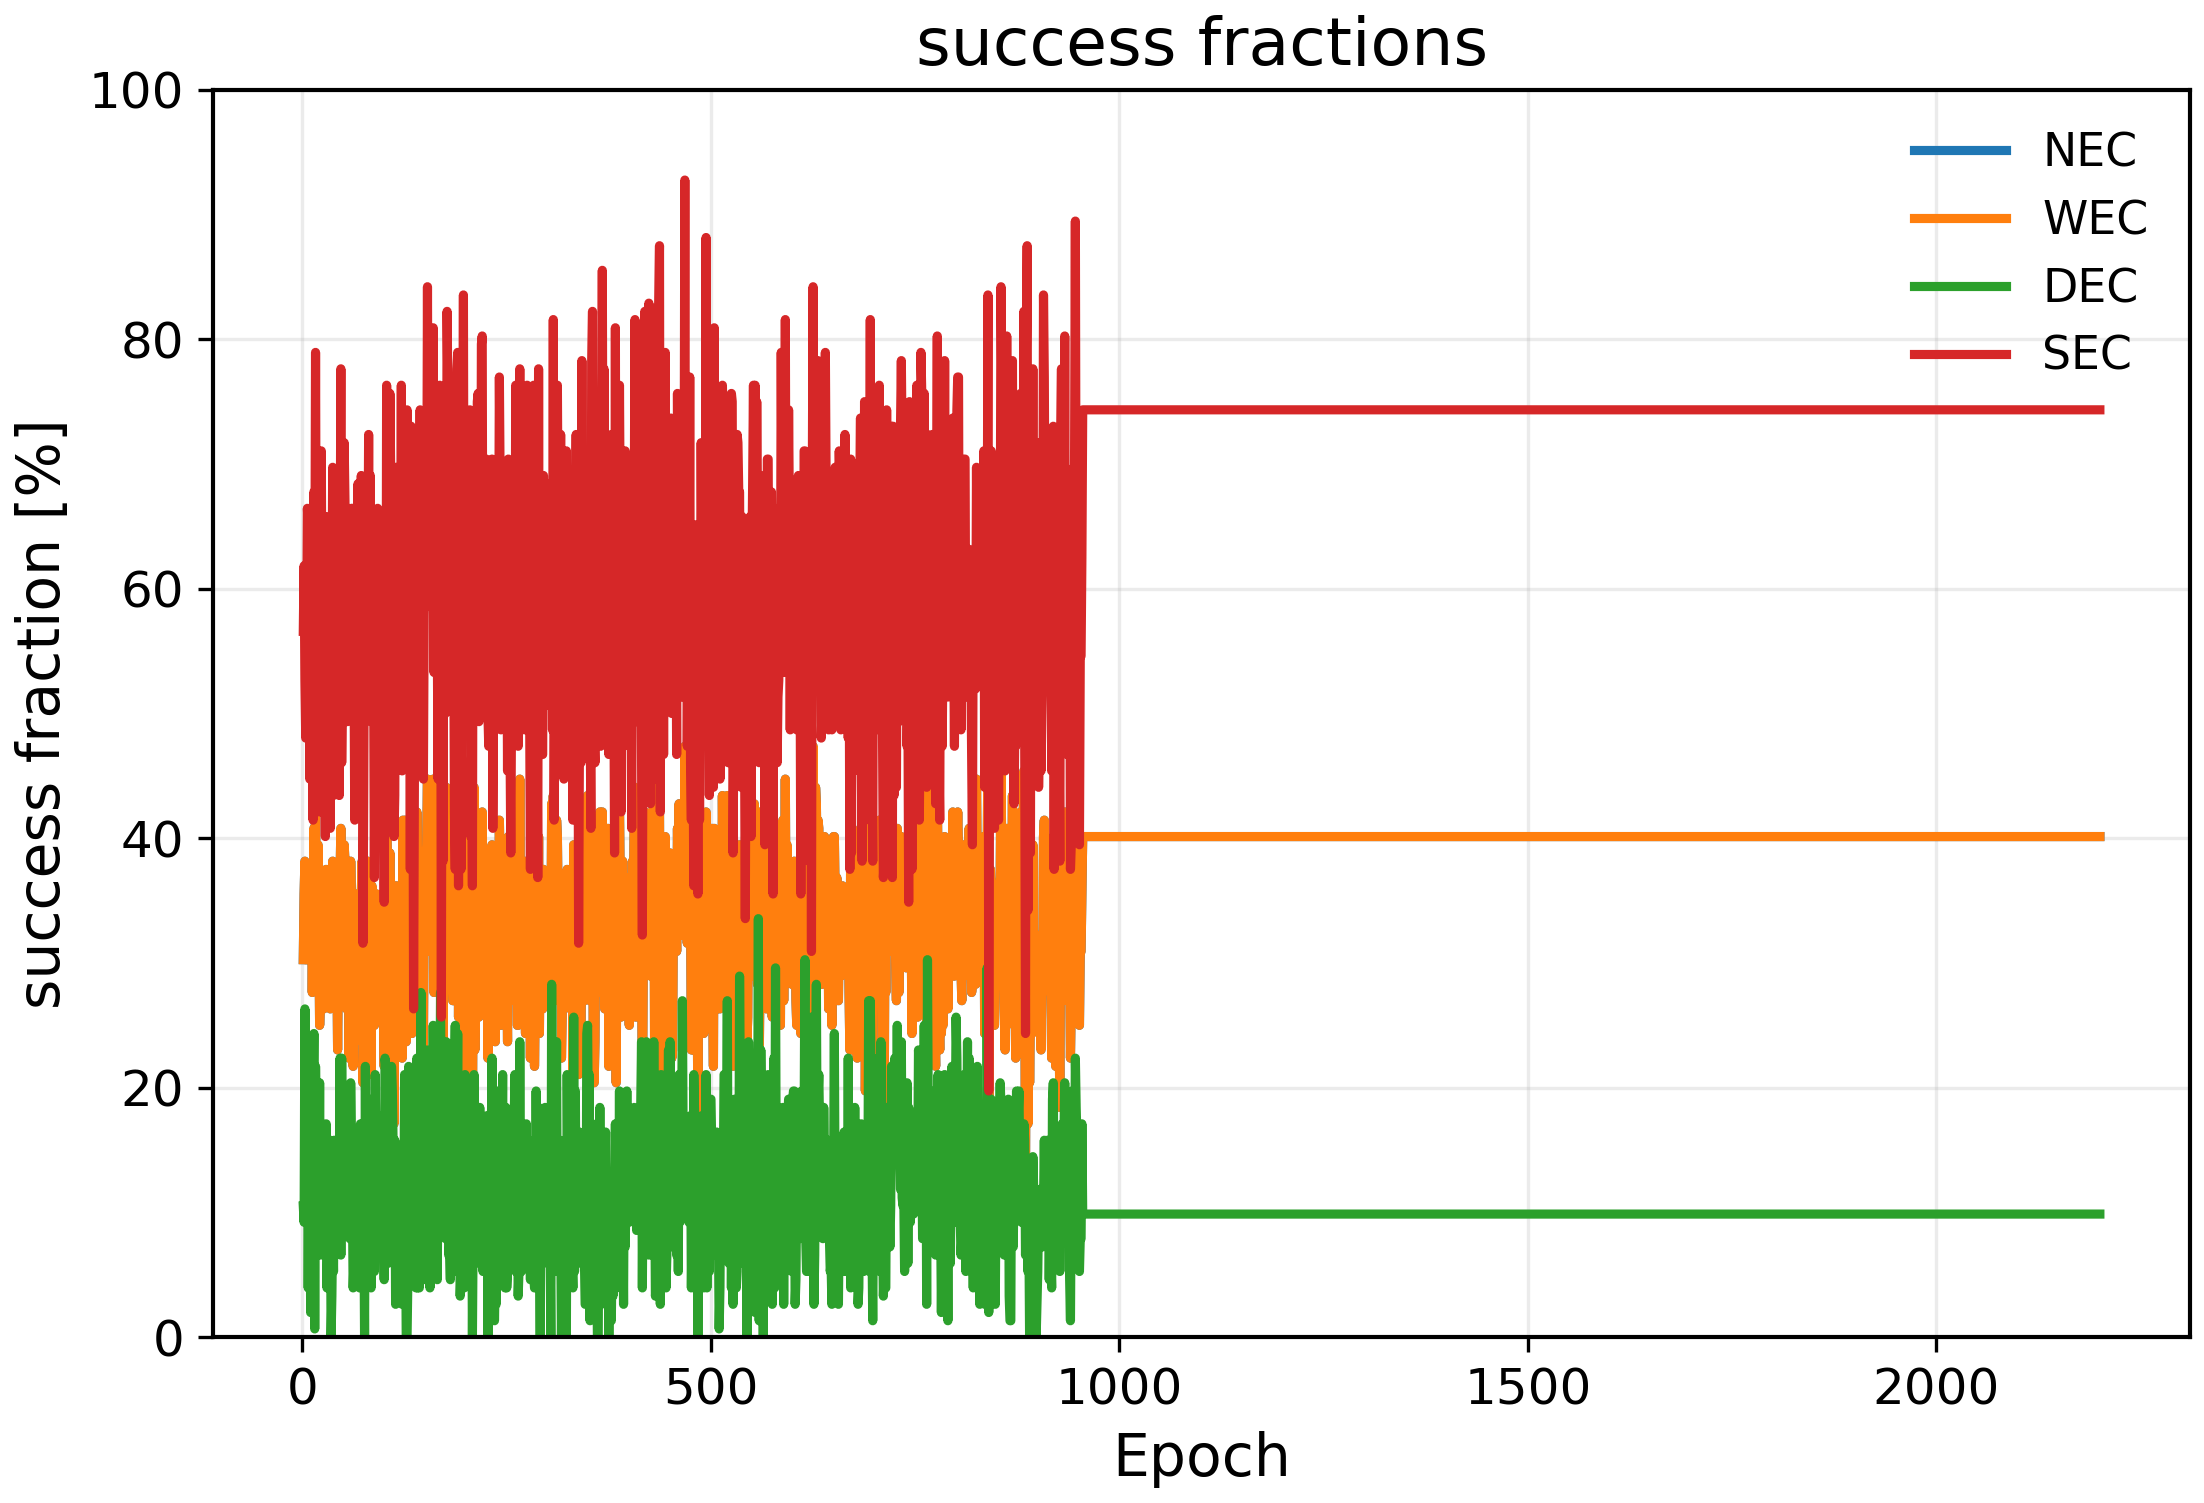
\includegraphics[width=\linewidth]{figures/domain_2_v_0p1_t_30p0_success_fractions.png}
    \caption{Success fractions for NEC/WEC/DEC/SEC.}
    \label{fig:d2-success}
  \end{subfigure}

  \vspace{1ex}

  \begin{subfigure}[t]{0.62\textwidth}
    \centering
    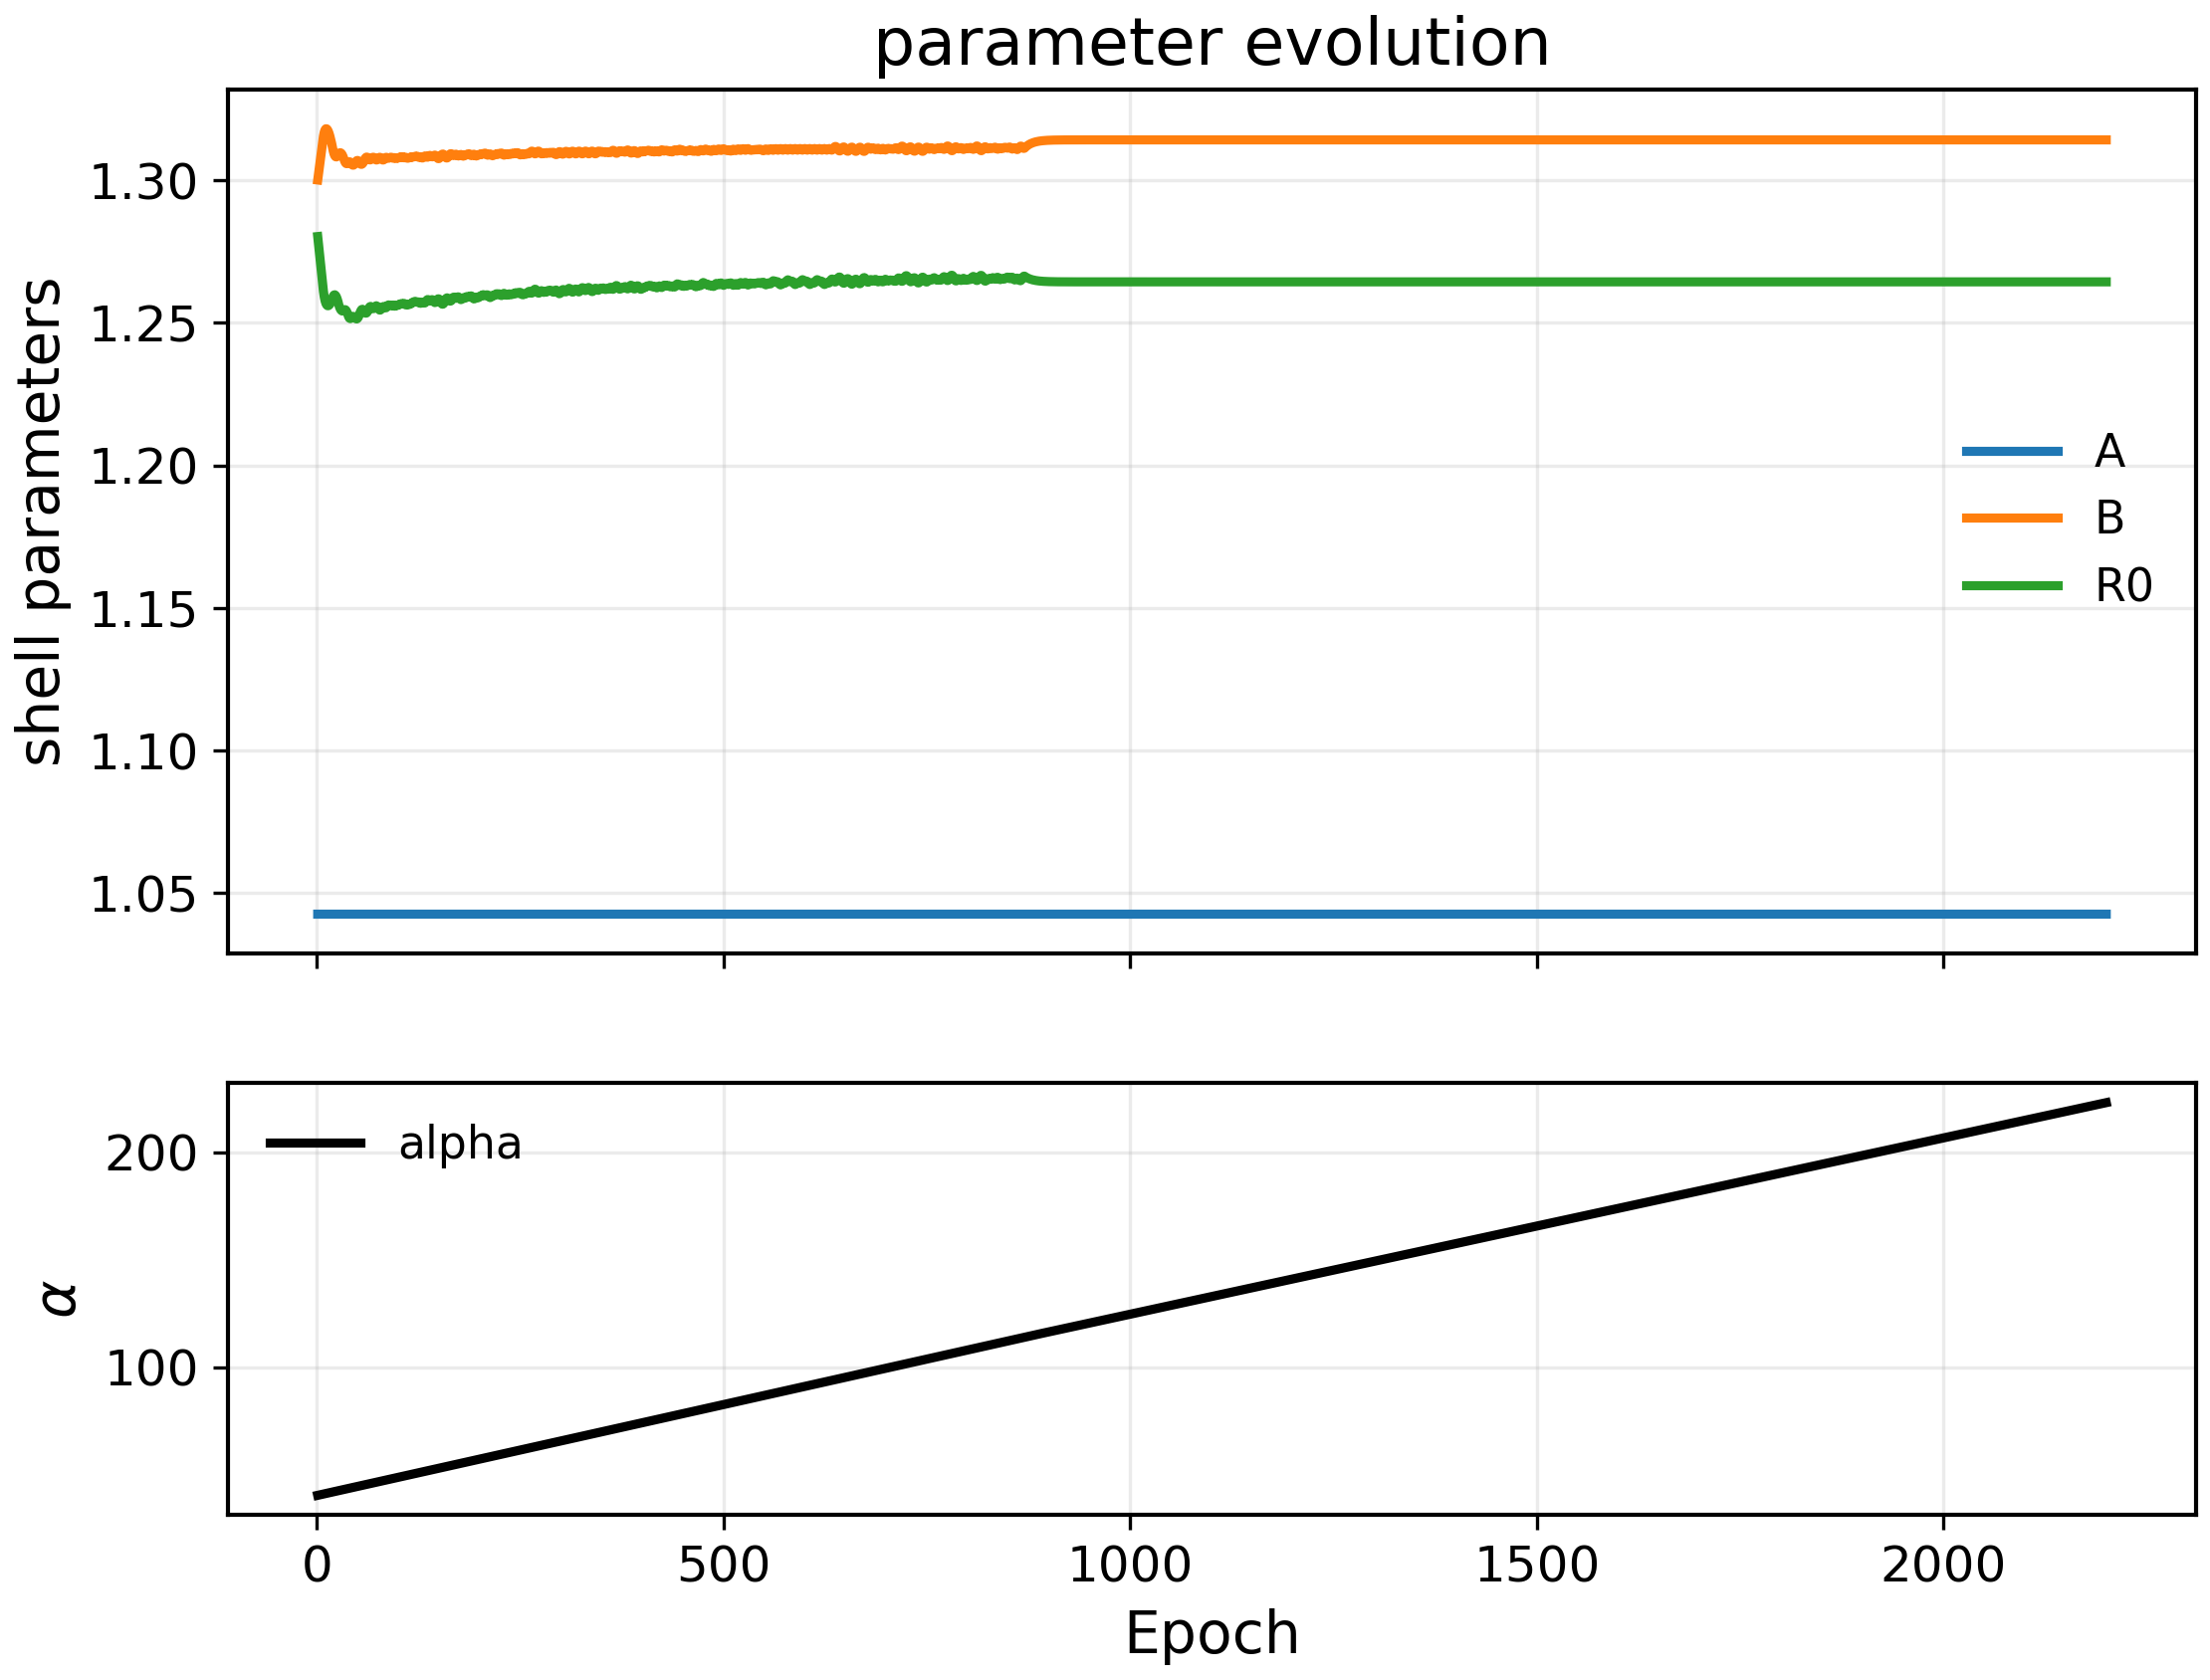
\includegraphics[width=\linewidth]{figures/domain_2_v_0p1_t_30p0_params.png}
    \caption{Seed parameters $A$, $B$, and $R_0$ across epochs.}
    \label{fig:d2-params-epoch}
  \end{subfigure}

  \caption{Optimization diagnostics for the double-shell configuration at $v=0.1$, $t=30$. Panel (a) shows the normalized loss terms \texttt{inv\_alpha}, \texttt{physics\_loss}, \texttt{reg\_breach}, and \texttt{total\_loss}. Panel (b) reports the fractions of grid points satisfying NEC/WEC/DEC/SEC; the double-shell case settles into a constrained regime in which SEC remains the easiest condition to satisfy, NEC/WEC stay above DEC, and DEC remains the tightest global constraint. Panel (c) shows that after a modest early adjustment the main run remains in a narrow band of $A$, $B$, and $R_0$, indicating a stable but more strongly constrained configuration within the adopted loss and diagnostic choices.}

  \label{fig:d2-opt}
\end{figure}


\FloatBarrier

\section*{Code and Data Availability}
The cleaned optimization, diagnostics, plotting, and verification workflow used in this study is publicly archived at Zenodo~\citep{Bolivar_Abellan_Vasilev_2026_warp_optimization}, DOI: \url{https://doi.org/10.5281/zenodo.19040071}. The archive includes the source code, the regenerated single-shell and double-shell golden bundles used for the manuscript-level claims, and direct evaluations of the manuscript target parameters under the same diagnostics. These materials are sufficient to reproduce the reported bundle summaries and field-map figures.

\bibliographystyle{unsrtnat}
\bibliography{warpdrive1}

\end{document}







